\documentclass[% 
reprint,
superscriptaddress,
%groupedaddress,
%unsortedaddress,
%runinaddress,
%frontmatterverbose, 
%preprint,
%showpacs,preprintnumbers,
%nofootinbib,
%nobibnotes,
%bibnotes,
 amsmath,amssymb,amsfonts,
 aps,
 pra,
 longbibliography
%prb,
%rmp,
%prstab,
%prstper,
%floatfix,
]{revtex4-2}

\newcommand{\ket}[1]{\ensuremath{|{#1}\rangle}}
\newcommand{\bra}[1]{\ensuremath{\langle{#1}|}}
\newcommand{\sca}[2]{\ensuremath{\bigl({#1}\cdot{#2}\bigr)}}
\newcommand{\avr}[1]{\ensuremath{\langle{#1}\rangle}}

\newcommand{\cnj}[1]{{#1}^{\ast}}
\newcommand{\hcnj}[1]{{#1}^{\dagger}}
\newcommand{\tcnj}[1]{{#1}^{T}}

%Differential operators

\newcommand{\prt}[1]{\partial_{#1}}
\newcommand{\pdrs}[1]{\partial_{#1}}
\newcommand{\pdr}[2]{\frac{\partial #1}{\partial #2}}
\newcommand{\drf}[2]{\frac{\dd #1}{\dd #2}}
\newcommand{\vdr}[2]{\dfrac{\delta #1}{\delta #2}}

\newcommand{\ddiv}{\mathop{\rm div}\nolimits}
 \newcommand{\rrot}{\mathop{\rm rot}\nolimits}
 \newcommand{\grad}{\mathop{\rm grad}\nolimits}
\newcommand{\bnbl}{\boldsymbol{\nabla}}

%Functions

\newcommand{\diag}{\mathop{\rm diag}\nolimits}
\newcommand{\sign}{\mathop{\rm sign}\nolimits}
\renewcommand{\Re}{\mathop{\rm Re}\nolimits}
\renewcommand{\Im}{\mathop{\rm Im}\nolimits}
\newcommand{\Tr}{\mathop{\rm Tr}\nolimits}
\newcommand{\ad}{\mathop{\rm ad}\nolimits}
\renewcommand{\ker}{\mathop{\rm Ker}\nolimits}

\newcommand{\cn}{\mathop{\rm cn}\nolimits}
\newcommand{\sn}{\mathop{\rm sn}\nolimits}
\newcommand{\dn}{\mathop{\rm dn}\nolimits}

%Units

\newcommand{\mum}{$\mu$m}
\newcommand{\dega}{$^\circ$}
\newcommand{\degc}{$^\circ$C}
\newcommand{\myarrow}[1]{\ensuremath{\xrightarrow{{#1}^\circ\mathrm{C}}}}

%Symbols

 \newcommand{\bs}[1]{\boldsymbol{#1}}
 \newcommand{\vc}[1]{\mathbf{#1}}
 \newcommand{\mvc}[1]{\mathbf{#1}}
 \newcommand{\uvc}[1]{\hat{\mathbf{#1}}}
 \newcommand{\ubs}[1]{\hat{\boldsymbol{#1}}}
 \newcommand{\ind}[1]{\mathrm{#1}}
\newcommand{\oprt}[1]{\ensuremath{\widehat{\mathcal{#1}}}}

%% 1. Math
\newcommand{\prob}{\mathsf{P}}
\newcommand{\dd}{\mathrm{d}}
\newcommand{\DD}{\ensuremath{\mathcal{D}}}
\newcommand{\JJ}{\ensuremath{\mathcal{J}}}
 \newcommand{\e}{\mathrm{e}}
 \newcommand{\ee}{\mathrm{e}}
\newcommand{\sts}{\ensuremath{\mathcal{Z}}}

\newcommand{\eff}{\mathrm{eff}}
\newcommand{\mx}{\mathrm{max}}
\newcommand{\mn}{\mathrm{min}}

\usepackage[english]{babel}
\usepackage[utf8x]{inputenc}
\usepackage[T1]{fontenc}


%% Useful packages
\usepackage{amsmath}
%\usepackage[colorinlistoftodos]{todonotes}
%\usepackage[colorlinks=true, allcolors=blue]{hyperref}
\usepackage{amssymb,amsmath,amsthm,mathtools,mathrsfs}
\usepackage{graphicx}% Include figure files
\usepackage{multirow}% Include figure files
\usepackage{float}% Include figure files
\usepackage{subcaption}% Include figure files


%\graphicspath{{figs/}}
\renewcommand{\floatpagefraction}{0.8}

%\selectlanguage{english}

\usepackage{soul,color}
\begin{document}
\DeclareGraphicsExtensions{.png,.pdf}
\title{
  Asymmetry effects in homodyne-like measurements:
Gaussian approximation and positive operator-valued measures
}

\author{A. S.~Naumchik}
\email[Email address: ]{naumchik95@gmail.com}
\affiliation{ITMO University, Kronverksky Pr. 49, Saint Petersburg  197101, Russia}


\author{Roman~K.~Goncharov}
\email[Email address: ]{toloroloe@gmail.com}
\affiliation{ITMO University, Kronverksky Pr. 49, Saint Petersburg  197101, Russia}


\author{Alexei~D.~Kiselev}
\email[Email address: ]{alexei.d.kiselev@gmail.com}
\affiliation{Laboratory of Quantum Processes and Measurements, ITMO
  University, Kadetskaya Line 3b, Saint Petersburg 199034, Russia} 
\affiliation{Leading Research Center "National Center for Quantum Internet", ITMO University,
  Birzhevaya Line 16, Saint Petersburg 199034, Russia}

\date{\today}

\begin{abstract}
  We study applicability of
  the Gaussian approximation describing
  photon count statistics for both the homodyne and the double homodyne
  measurements in the presence of asymmetry effects when
  the beam splitters are unbalanced and the quantum efficiencies of
  the photodetectors are not identical.
We also use the Gaussian approximation to construct
the positive operator-valued measure (POVM) that takes into account the asymmetry effects. 
It is found that, when the Skellam distribution is approximated using the asymptotic expansions of
modified Bessel functions for large argument,
the asymmetry effects lead to ill-posed Gaussian POVM.
\end{abstract}
 
 \maketitle

%%%%%%%%%%%%%%
\section{Introduction}
\label{sec:intro}
%%%%%%%%%%%%%%


Homodyne measurement is an important example of Gaussian measurements and is widely applied in
continuous-variable quantum key distribution (CV-QKD) systems
\cite{PhysRevLett.88.057902,PhysRevLett.93.170504,RevModPhys.84.621,e17096072,opt3040030,Zhang:apr:2024}.
This
measurement traditionally involves a beam splitter (BS), where the two input ports are occupied by
the signal and reference modes, and the two output ports are detected by quantum detectors (see
Fig.~\ref{fig:homodyne}).  To simplify calculations, one can consider the reference mode to be much
stronger in amplitude than the signal, leading to the so-called strong Local Oscillator (LO)
approximation. For the resulting statistical distribution to accurately describe a real physical
process, it is necessary to construct the corresponding positive-valued operator measure (POVM).

\textcolor{red} {\textbf{Balanced homodyne:} In
  Ref.~\cite{PhysRevA.51.4160} a study of potential benefits of using
  weak LO (of same amplitude as signal) is conducted. Description is
  focused on correlation functions, and considers 2 schemes: homodyne
  intensity correlation scheme, consisting of $2$ BS, the intensity
  correlations are measured with $2$ photodetectors, and homodyne
  cross correlation scheme with $1$ BS (not $50:50$). These schemes
  are of particular interest in cases where low overall efficiencies
  prevent the detection of phase-sensitive effects by standard
  balanced or unbalanced homodyning. Strong LO does not allow for
  observing squeezing effect, and LO noise is not balanced out. Small
  classical excess noise of the LO is amplified when its strong, so
  detection of squeezed light is not possible. On the contrary, using
  weak LO, relative squeezing is much larger and therefore easier to
  observe, new phase-sensitive effects can be observed as well: the
  normally ordered intensity variance, the normally ordered field
  strength variance, and the normally ordered correlation of the
  intensity and field strength fluctuations. The corresponding
  spectral properties can be recorded by the homodyne correlation
  schemes: the spectrum of intensity fluctuations, the squeezing
  spectrum, the correlation spectrum of field strength and intensity
  fluctuations. Last one gives the spectral correlation of two
  noncommuting observables. And decreasing LO results in lesser
  classical noise. Detectors must be of high efficiency to detect
  these signals, and signals need to be temporally stable.  Balanced
  homodyning is insensitive to local-oscillator quadrature-phase noise
  and hence provides (1) a means of detecting reduced quadrature-phase
  fluctuations (squeezing) that is perhaps more practical than
  one-port homodyning and (2) an output signal-to-noise ratio that can
  be a modest to significant improvement over that of unbalanced
  homodyning and direct detection \cite{Schumaker:84}. In addition to
  the unavoidable quantum fluctuations, it is shown that excess noise
  from the local oscillator always affects homodyning and, when it is
  broadband, also heterodyning. Both the quantum and the excess noise
  of the local oscillator can be eliminated by coherent subtraction of
  the two outputs of a 50/50 beam splitter \cite{Yuen:83}. Excess
  intensity noise in the local oscillator can be canceled
  \cite{Abbas:83}.  }
        
\textcolor{red}{\textbf{Unbalanced:}
        Ref.~\cite{PhysRevA.53.4528} discusses the technique of
        unbalanced homodyne detection (only one output port of the BS
        is detected). It shows that reconstructing the quantum state
        of the signal field from the photocounting statistics recorded
        in this scheme (related to $s$-parametrized quasiprobability
        distributions) is possible for $s<1$. To do so, POVM is
        derived. 
        Practically this is difficult to realize: the noise is
        significant,  presently available photomultipliers have small
        efficiencies, so that the applicability of the method might be
        presently limited to the reconstruction of smooth
        quasiprobability distributions. A possible solution is to use
        of an array of highly efficient avalanche photodiodes instead
        of photon count detectors \cite{PhysRevA.53.4528,
          PhysRevA.101.031801}. Naturally, theoretical description
        (photon count formula) is to be modified as well
        \cite{PhysRevA.85.023820,PhysRevA.92.053835} to account for
        number of detectors (and dark photon counts).  
Quality of the results of reconstruction are affected by quantum
detector efficiency, being less accurate for lower efficiencies.} 

\textcolor{red}{
\textbf{Double homodyne:}
        Ref.~\cite{Cives_Esclop_2000} discusses the the double
        homodyne scheme with finite LO intensity. The paper
        demonstrates how the eight-port detector can be used to
        reconstruct the quantum state of the signal field, even when
        the LO intensity is not significantly larger than the
        signal. Analysis of limits of weak LO and strong LO is given
        as well: for strong LO they obtain the $Q$-function of the
        signal state, and for weak LO the phase is lost and they only
        able to measure the probability distribution for the photon
        number. Classical treatment of the homodyne is given as well. 
}

\textcolor{red}{\textbf{LO of other states:}
In Ref.~\cite{combes2022homodyne},  Schr\"odinger cat states (even and
odd) of finite amplitude are considered as local oscillators of a
standard homodyne scheme. Since LO state is not Gaussian, this
measurement scheme is not Gaussian as well. This scheme allows for
preparation of non-Gaussian states.}. 

\textcolor{red}{
In the context of \textbf{quantum random number generators} (QRNGs),
accounting for measurement imperfections is of great importance for
ensuring the reliability and security of the generated random
numbers. As demonstrated in Ref.~{\cite{haw2015maximization}},
classical noise plays a significant role in influencing the entropy of
the random numbers generated, as well as leading to potential
vulnerabilities, as it can be tampered with. Our results suggest that
homodyne measurement imperfections are alike to classical noise in the
sense of affecting the variance of the output, meaning similar
conclusions of the performance of QRNG may be drawn. 
}

\textcolor{blue}{For ideal homodyne and double homodyne detection
  schemes with unequal detector efficiencies, POVMs are well-known,
  being the projectors onto quadrature operators and superposition of
  these projectors, respectively.  
However, practical applications have imperfections~\cite{hajomer2025finite}. 
Although accounting for BS imbalance in the formulae is conceptually
simple, the calculations have not been carried out
explicitly. Additionally, similar projectorsconsiderations have not
been applied to the double homodyne scheme. Considering
photon-counting schemes, detection imperfections are not only losses,
but photon number resolution
\mbox{~\cite{len2022realistic,yeremenko2024realistic}} and detector
dead time \mbox{~\cite{ len2022realistic, reutov2021photon}}. These
imperfections are beyond the scope of this work.} 

\textcolor{blue}{Critical cases of asymmetry in homodyne scheme were
  discussed previously. Ref.~\cite{PhysRevA.53.4528} discusses the
  technique of unbalanced homodyne detection (in the sense of only one
  quantum detector used as opposed to traditionally detecting both
  output ports of BS). It shows that reconstructing the quantum state
  of the signal field from the photocounting statistics recorded in
  this scheme (related to $s$-parametrized quasiprobability
  distributions) is possible. Quality of the results of reconstruction
  are affected by quantum detector efficiency, being less accurate for
  lower efficiencies. However,  
this scheme is difficult to realize, as the effect of classical noise
is significant, and presently available photomultipliers have small
efficiencies, so that the applicability of the method might be
limited. A possible solution is to use of an array of highly efficient
avalanche photodiodes instead of photon count
detectors\mbox{~\cite{PhysRevA.53.4528,
    PhysRevA.101.031801}}. Naturally, theoretical description (photon
count formula) is to be modified as well
\mbox{\cite{PhysRevA.85.023820,PhysRevA.92.053835}}. These studies
focus on the critical case of imbalance (one of the detector ports
being unused) for specific measurement purposes. In this sense, the
case with an unused port can be interpreted as corresponding to zero
efficiency.} 

\textcolor{blue}{
Numerical studies of photon count distributions for different signal
states in homodyne schemes have been performed
{~\cite{freyberger1993photon}}. In that work, photon difference
distributions for Fock signal states were analyzed, and the dependency
on detector efficiencies was studied. However, the dependency of the
quality of the LO approximation compared to the exact distribution was
not quantified. A numerical study on the role of the LO intensity in
an imperfect homodyne scheme has been conducted in
Ref.{~\cite{OLIVARES2020126354}}. In this scheme, the homodyne setup
has non-unity, equal quantum detectors and a balanced BS. It shows
that a strong LO is not required to reconstruct a quantum state; a
low-intensity LO can provide a reconstruction with sufficient
fidelity, which increases as the LO intensity increases.} 

\textcolor{green}{Device imperfections play a significant role in continuous-variable quantum key distribution (CV-QKD). In Ref.~\cite{ruiz2023effects} a CV-QKD system is modeled numerically using a classical description of electromagnetic fields to investigate the impact of device imperfections on the secure key rate. Specifically, a non-ideal beam splitter and an unbalanced detector are considered. The study reveals that these imperfections lead to a reduction in the secure key generation rate. However, this analysis is based on a classical, rather than quantum, description of the system, which may limit the accuracy of the results.}

Our analysis focuses on the case of an unbalanced beam splitter and unequal non-unity quantum
efficiency of photodetectors, which we refer to as the asymmetrical case, in contrast to the
traditionally studied symmetrical case of a balanced beam splitter and equal non-unity quantum
efficiencies. To obtain the approximation, we approximate the Poisson distribution with the Gaussian
distribution, which will be referred to as Gaussian approximation. We will use the LO approximation
to further simplify the resulting function. After this, we construct the respective POVM and
numerically study the quality of the approximation. We apply developed formalism to another
homodyne-based detection scheme, namely double homodyne scheme (also known as heterodyne scheme in
the QKD literature~\cite{Pirandola:20,opt3040030,Zhang:apr:2024}), to demonstrate its applicability. \textcolor{red}{We find that for the asymmetrical double homodyne POVM an extension to the set of squeezed coherent states is required. The results for asymmetrical measurements are then used to calculate the CV-QKD asymptotic secret fraction to estimate the impact of measurement asymmetry on protocol security.}

Our findings also reveal that the usual approach of approximating the Skellam distribution using the
asymptotic expansion of the modified Bessel function of the first kind is not applicable in the
asymmetrical case.

The paper is organized as follows.  In Sec.~\ref{sec:homodyne} we obtain the statistical
distribution of difference photon counts in Gaussian approximation, from which we obtain the
respective POVM. We thoroughly analyze the dependence of the statistical distribution on the asymmetry
parameters.  In Sec.~\ref{sec:double-homodyne} we conduct the analysis of the double homodyne scheme
analogously to the previous section, finding out that the resulting POVM is not well defined for all asymmetry parameters, requiring generalization.
\textcolor{red}{
In Sec.~\ref{sec:gen-POVM} we generalize the double homodyne POVM to the set of squeezed coherent states. 
In Sec.~\ref{sec:protocol} we apply our results for homodyne and double homodyne detection to calculate the asymptotic secret fraction for an ideal CV-QKD system. }
% In Sec.~\ref{sec-experiment} a number of experiments are performed
% and the experimental results are analyzed. 
% xd
Finally, in Sec.~\ref{sec:conclusion} we conclude the paper with a brief summary of the results and
suggestions for future development.

\begin{figure}
    \centering
    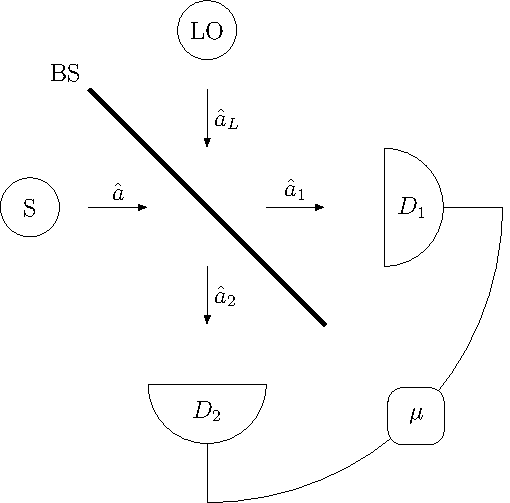
\includegraphics[width=0.9\linewidth]{pics/schemes/homodyne.pdf}
    \caption{Scheme of a homodyne receiver: S is the source of the
      signal mode with the annihilation operator $\hat{a}$,
      LO is the source of the reference mode (local oscillator) with the annihilation
      operator $\hat{a}_{L}$, and BS is the beam splitter with
      the amplitude transmission and reflection coefficients
      $t=\cos\theta$ and $r=\sin\theta$, respectively; photodetectors $D_1$ and $D_2$ have quantum efficiencies
     $\eta_{1}$ and $\eta_{2}$, and $\mu\equiv m_1-m_2$ is the photon count
      difference.}
    \label{fig:homodyne}
\end{figure}

%%%%%%%%%%%%%%%%%%%%%%%%%%%%
\section{Homodyne detection}
\label{sec:homodyne} 
%%%%%%%%%%%%%%%%%%%%%%%%%%%

%%%%%%%%%%%%%%%%%%%%%%%%%%%%%
\subsection{Gaussian approximation}
\label{subsec:gauss-hom}
%%%%%%%%%%%%%%%%%%%%%%%%%%%%%%


We begin with brief discussion
of the homodyne measurement setup
schematically depicted in Fig.~\ref{fig:homodyne}.
To this end, we assume that the beam spitter is unbalanced
and its scattering matrix is chosen to be a real-valued
rotation matrix with the transmission and reflection amplitudes,
$t$ and $r$, given by
\begin{align}
  \label{eq:BS-amplitudes}
  t=\cos\theta\equiv C,
  \quad
  r=\sin\theta\equiv S.
\end{align}
Then the input coherent states
of the signal mode and the local oscillator 
are transformed into the output coherent states
as follows
\begin{align}
  \label{eq:BS}
  &
    \ket{\alpha,\alpha_L}\mapsto\ket{\alpha_1,\alpha_2},
  \\
  &
    \label{eq:amplitudes}
    \alpha_1=C\alpha+S\alpha_L,\quad
    \alpha_2=-S\alpha+C\alpha_L,
\end{align}
so that
the joint probability of $m_1$ and $m_2$ photon counts
for the photodetectors $D_1$ and $D_2$
can be computed from the well-known Kelley-Kleiner formula~\cite{Kelley:pr:1964}
(see also Ref.~\cite{Vogel:pra:1993}):
\begin{align}
  &
    \label{eq:1}
    \prob(m_1,m_2)=
    \bra{\alpha_1,\alpha_2}:\prod_{l=1}^{2}\frac{(\eta_l\hat{n}_l)^{m_l}e^{-\eta_l\hat{n}_l}}{m_l!}:\ket{\alpha_1,\alpha_2}
    \notag
  \\
  &
 =\prod_{l=1}^{2}\frac{(\eta_l|\alpha_l|^2)^{m_l}}{m_l!}e^{-\eta_l|\alpha_l|^2}    
\end{align}
where
$:\ldots:$ stands for normal ordering,
index $l\in\{1,2\}$ labels output ports of the beam splitter,
$\hat{n}_l=\hcnj{\hat{a}}_l\hat{a}_l$ is the photon number operator,
$m_l$ is the number of photon counts,
$\eta_l$ is the quantum efficiency of the detector $D_l$.

% and
% $|\alpha_l|$ are the transformed amplitudes, given by
% \begin{align}
%   \label{eq:amplitudes1}
%   &
%         \cos \theta\equiv C,\quad 
%                       \sin \theta\equiv S,
% \notag
%   \\
%   &
%     \alpha_1=C\alpha+S\alpha_L,\quad
%     \alpha_2=-S\alpha+C\alpha_L,
% \end{align}
% with the
We can now introduce the photon count difference
\begin{equation}
  \label{eq:dleta-m}
    \mu = m_1-m_2
  \end{equation}
  so that its statistical distribution %of the photon count difference
  can be written in
  the form of a product of the two Poisson distributions as follows 
\begin{align}
  &
\label{eq:poisson}  
    \prob(\mu) =\sum_{m_2=\max(0,-\mu)}^{\infty}
    \frac{(\eta_1|\alpha_1|^2)^{\mu+m_2}}{(\mu+m_2)!}e^{-\eta_1|\alpha_1|^2}
    \notag
  \\
  &
    \times
\frac{(\eta_2|\alpha_2|^2)^{m_2}}{m_2!}e^{-\eta_2|\alpha_2|^2}.
\end{align}
It is well known that, by performing summation over $m_2$,
the probabilty $\prob(\mu)$ reduces to
the Skellam distribution given by~\cite{skellam1946frequency}
\begin{align}
  &
  \label{eq:accurate}
  \prob(\mu)=e^{-\eta_1|\alpha_1|^2}e^{-\eta_2|\alpha_2|^2}
    \Biggl(\frac{\eta_1|\alpha_1|^2}{\eta_2|\alpha_2|^2}\Biggr)^{\mu/2}
    \notag
  \\
  &
    \times
I_{\mu}\bigl(2\sqrt{\eta_1\eta_2|\alpha_1|^2|\alpha_2|^2}\bigr),
\end{align}
where $I_k(z)$ is the modified Bessel function of the first kind~\cite{NIST:hndbk:2010}.

An important point is that,
at sufficiently large
$|\alpha_1|$ and $|\alpha_2|$,
Poisson distributions that enter Eq.~\eqref{eq:1}
can be approximated using
the probability density functions of the normal distributions
with mean and variance both equal to the mean of
the corresponding Poisson distribution, $\lambda_i=\eta_i |\alpha_i|^2$.
Then, in the continuum limit where
summation in Eq.~\eqref{eq:poisson} is replaced with integration,
the Skellam distribution~\eqref{eq:accurate}
can be approximated assuming
that the amplitude of the local oscillator, $|\alpha_L|$, is large
(the strong LO approximation) and
we can apply the convolution formula
for Gaussian probability densities
\begin{align}
  &
  \label{eq:convolution}
  \int G(x_1-x_2;\sigma_1)G(x_2;\sigma_2)\dd
    x_2=G(x_1;\sigma_1+\sigma_2),
  \\
  &
    \label{eq:G-notation}
    G(x;\sigma)\equiv\frac{1}{\sqrt{2\pi\sigma}}\exp\Bigl(-\frac{x^2}{2\sigma}\Bigr).
\end{align}

The above procedure
immediately leads to the Gaussian approximation
of the form:
\begin{align}
  &
  \label{eq:Gaussian}
    \prob_G(\mu)=G(\mu-\mu_G;\sigma_G),
    \\
  &
    \label{eq:sigma_G}
    \sigma_G=\eta_1|\alpha_1|^2+\eta_2|\alpha_2|^2
    \approx
    (\eta_1S^2+\eta_2C^2) |\alpha_L|^2,
  \\
  &
    \label{eq:mu_G}
    \mu_G=\eta_1|\alpha_1|^2-\eta_2|\alpha_2|^2
    \approx
    (\eta_1S^2-\eta_2C^2) |\alpha_L|^2
    \notag
  \\
  &
    +CS (\eta_1+\eta_2) |\alpha_L| \avr{\hat{x}_\phi}
\end{align}
where
\begin{align}
  &
  \label{eq:avr-x-phi}
  \avr{\hat{x}_\phi}\equiv \bra{\alpha}\hat{x}_\phi\ket{\alpha}={2\Re\alpha e^{-i\phi}},
  \quad \phi=\arg\alpha_L
\end{align}
is the average of
the phase-rotated quadrature operator of the signal mode
given by
\begin{equation}
\hat{x}_\phi=\hat{a}e^{-i\phi}+\hat{a}^\dag e^{i\phi}.
    \label{eq:quad-op}
\end{equation}

Alternatively, the probability~\eqref{eq:Gaussian}
can be rewritten in the form
\begin{equation}
{\prob}_G(x)=\frac{1}{\sqrt{2\pi\sigma_G}}
    \exp \biggl\{-\frac{(x-\avr{\hat{x}_\phi})^2}{2\sigma_x}\biggr\},
    \label{eq:Pgood-w-def}
\end{equation}
where
$x$ is the quadrature variable given by
\begin{align}
  \label{eq:x-def}
  x\equiv\frac{\mu}{(\eta_1+\eta_2)CS|\alpha_L|}-\frac{\eta_1S^2-\eta_2C^2}{\left(\eta_1+\eta_2\right)CS}|\alpha_L|
\end{align}
and $\sigma_x$ is the quadrature variance
\begin{align}
  &
        \label{eq:sigma-x}
    \sigma_x\equiv
    \frac{\eta_1S^2+\eta_2C^2}{
    \left[(\eta_1+\eta_2)CS\right]^2
    }.
\end{align}
Note that it is rather straightforward to minimize
the variance~\eqref{eq:sigma-x} with respect to
the transmittance, $C^2$, and
deduce inequality
\begin{align}
  \label{eq:sigma-x-min}
  \sigma_x\ge \sigma^{(\min)}_{x}=\Biggl(
\frac{\sqrt{\eta_1}+\sqrt{\eta_2}}{\eta_1+\eta_2}
  \Biggr)^2\ge 1,
\end{align}
where $\sigma_x$ reaches its minimum value
$\sigma^{(\min)}_{x}$ at the beam splitter transmittance:
$C^2=\cos^2\theta_{\min}=\sqrt{\eta_1}/(\sqrt{\eta_1}+\sqrt{\eta_2})$.

\begin{figure*}[!htb]
  \centering
  \begin{subfigure}{0.49\textwidth}
    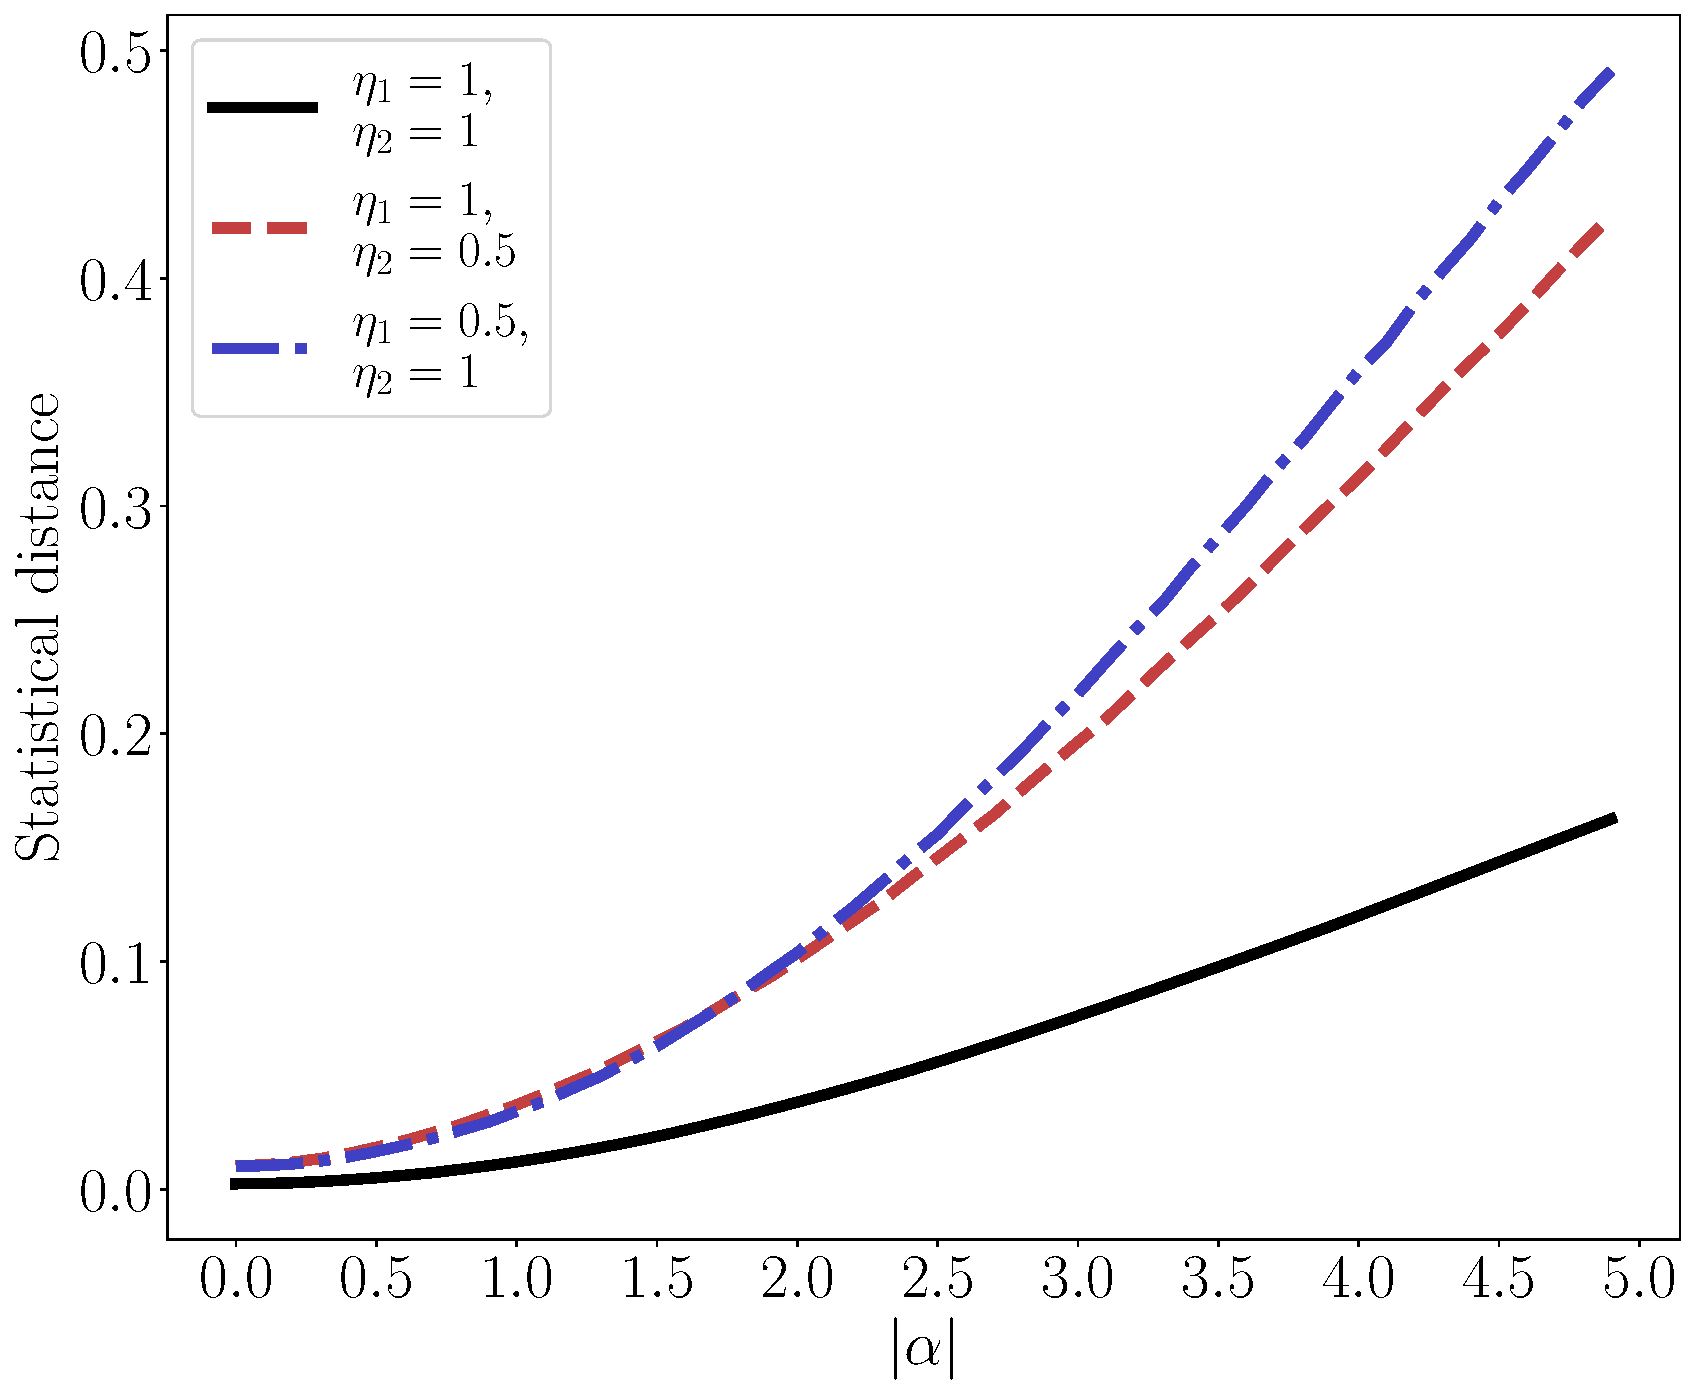
\includegraphics[width=\linewidth]{pics/homodyne/ED = ED(a)_eta.pdf}
    \caption{$|\alpha_L|=5$}
    \label{fig:amp_05}
\end{subfigure}
  \begin{subfigure}{0.49\textwidth}
    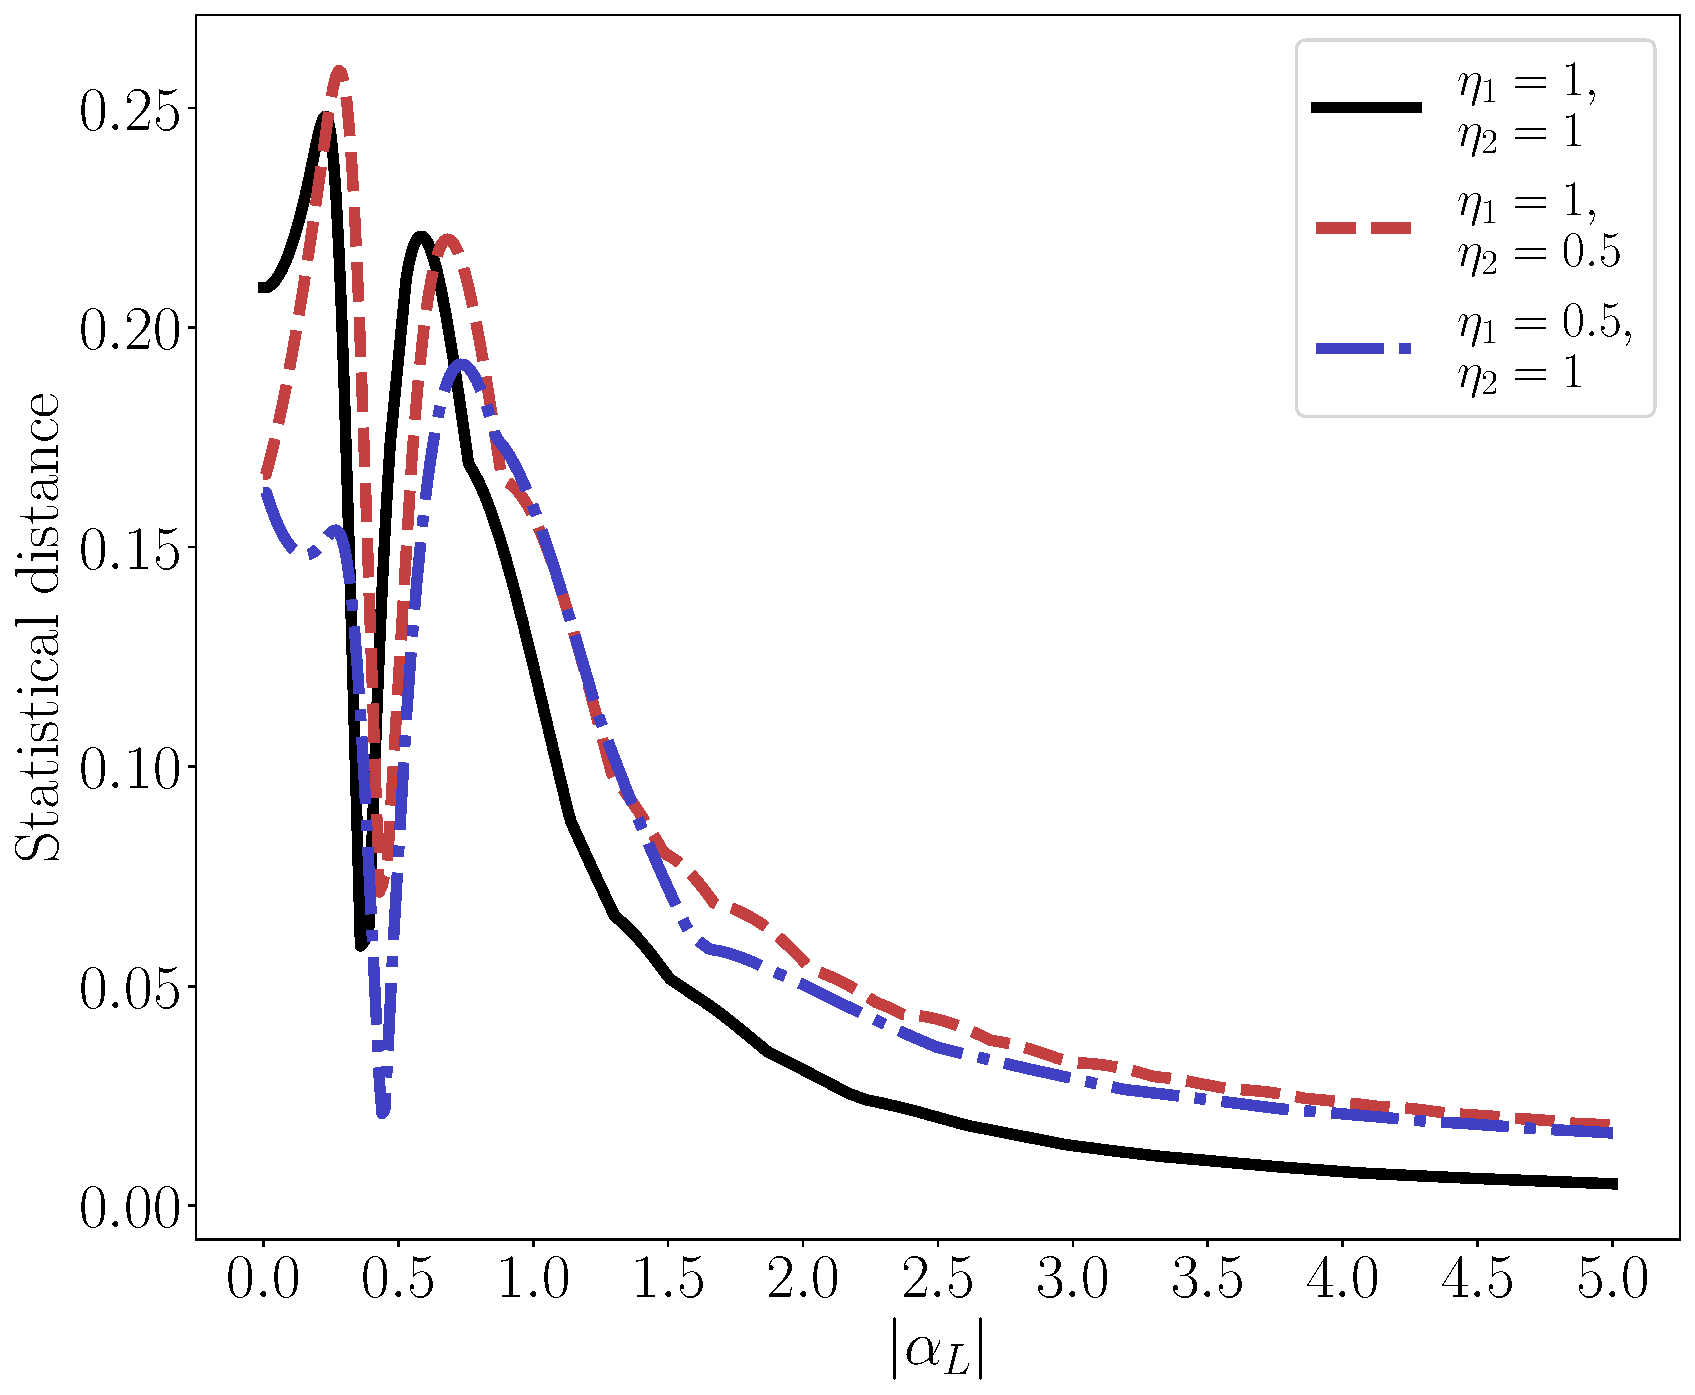
\includegraphics[width=\linewidth]{pics/homodyne/ED = ED(aL)_eta.pdf}
    \caption{$|\alpha|=0.5$}
    \label{fig:amp_01}
\end{subfigure}
\caption{
  Statistical distance $D_P=\mathtt{D}(\prob,\prob_G)$
  as a function of (a)~signal amplitude and (b)~LO amplitude at different
          detector efficiencies.
        }
  \label{fig:amplitude}
\end{figure*}


Our next step is to construct
the positive operator-valued measure
(POVM) based on the Gaussian approximation $\prob_G$.
To this end, note that the probability~\eqref{eq:Pgood-w-def}
%\eqref{eq:Pgood}
is the expectation value of the POVM in the coherent state
given by
\begin{equation}
  \label{eq:PG-as-avr}
    \prob_G=\langle\alpha|\hat{\Pi}_G|\alpha\rangle.
\end{equation}
In the case of
the perfectly symmetric homodyne measurement with
$\eta_1=\eta_2=1$ and $C=S=1/\sqrt{2}$,
the average~\eqref{eq:PG-as-avr}
takes the form
\begin{equation}
    \label{eq:P_0}
    \prob_G^{(0)}=
    \frac{1}{|\alpha_L|} Q_{x,\phi}(\alpha), 
  \end{equation}
  where
  $x=\mu/|\alpha_L|$
  and $Q_{x,\phi}(\alpha)$ is the Husimi $Q$ distribution
for the eigenstate of the phase-rotated quadrature
operator~\eqref{eq:quad-op},
$\ket{x,\phi}$, given by
(see, e.g., the textbook\cite{Vogel:bk:2006})
\begin{align}
  &
    \label{eq:Q-x}
  Q_{x,\phi}(\alpha)=
    |\langle \alpha|x , \phi \rangle |^2 =G(x-\avr{\hat{x}}_\phi;1).
%    \frac{1}{\sqrt{2\pi}}\exp\left[-\frac{1}{2}\left(x  - \langle \hat{x}_\phi\rangle\right)^2\right]. 
\end{align}
Thus, we are led to the well-known result that POVM describing sharp homodyne measurements
in the Gaussian approximation is proportional to
a projector onto $|x,\phi\rangle$:
\begin{align}
  &
  \label{eq:POVM-P0}
    \hat{\Pi}_G^{(0)}=\frac{1}{|\alpha_L|}|x,\phi\rangle\langle x,\phi|,
\end{align}

In  a more general asymmetric case with $\eta_1\ne \eta_2$
and $C\ne S$,
the Gaussian-shaped probability $\prob_G$ can be represented
as a Gaussian superposition written as
a convolution of $P_{G}^{(0)}$ and a Gaussian function $G(x,\sigma_N)$.
By using the convolution identity~\eqref{eq:convolution},
we have
\begin{align}
  &
  \label{eq:theform}
  \prob_G(x)=\sqrt{\frac{\sigma_x}{\sigma_G}} \int G(x-x';\sigma_N)\prob_G^{(0)}(x')\dd x',
  \\
  &
  \label{eq:sgm_N}
     \sigma_N=\sigma_x-1\ge 0,  
\end{align}
where non-negativity of the variance $\sigma_N$
stems from Eq.~\eqref{eq:sigma-x-min}.
  This result immediately gives
  a general formula for the Gaussian approximation POVM 
\begin{align}
  &
\label{eq:homodyne-povm}    
    \hat{\Pi}_G=\frac{1}{(\eta_1+\eta_2)CS|\alpha_L|}
    \notag
  \\
  &
    \times
    \int \dd x' G(x-x'; \sigma_N)|x',\phi\rangle\langle x',\phi|.
\end{align}
Note that the variance $\sigma_N$
describes the excess noise that takes into account asymmetry effects.

In the limiting case of perfect homodyne,
we have
\begin{equation}
    \lim_{\sigma_x \to 1}G(x;\sigma_N)=\lim_{\sigma_N \to 0}G(x;\sigma_N)=\delta(x),
\end{equation}
where $\delta(x)$ is the Dirac $\delta$-function,
which is the expected behavior for
Eq.~\eqref{eq:theform} to hold .
Therefore, the constructed POVM~\eqref{eq:homodyne-povm}
is well-defined for all possible parameters of the homodyne scheme.

% \textit{The ability of the homodyne scheme to reconstruct the quadrature of the state is well known
% (see e.g. Ref.~\cite{liu2021homodyne}), which is showcased by Eq.~\eqref{eq:homodyne-povm}.
% }
  

Our concluding remark concerns an alternative method
to approximate Eq.~\eqref{eq:accurate}
with a Gaussian-shaped distribution
which is based on the asymptotic expansions of the modified Bessel functions.
In Appendix~\ref{sec:appendix} we show that, for the asymmetric homodyne scheme,
this method generally leads to ill-posed POVMs because
the corresponding quadrature variance
appears to be too small leading to negative
contribution of the excess noise. 


%%%%%%%%%%%%%%%%%%%%%%%%%%%%%
\subsection{Numerical results}
\label{subsec:num-hom}
%%%%%%%%%%%%%%%%%%%%%%%%%%%%%%

\begin{figure*}
    \centering
    \begin{subfigure}[]{.45\linewidth}
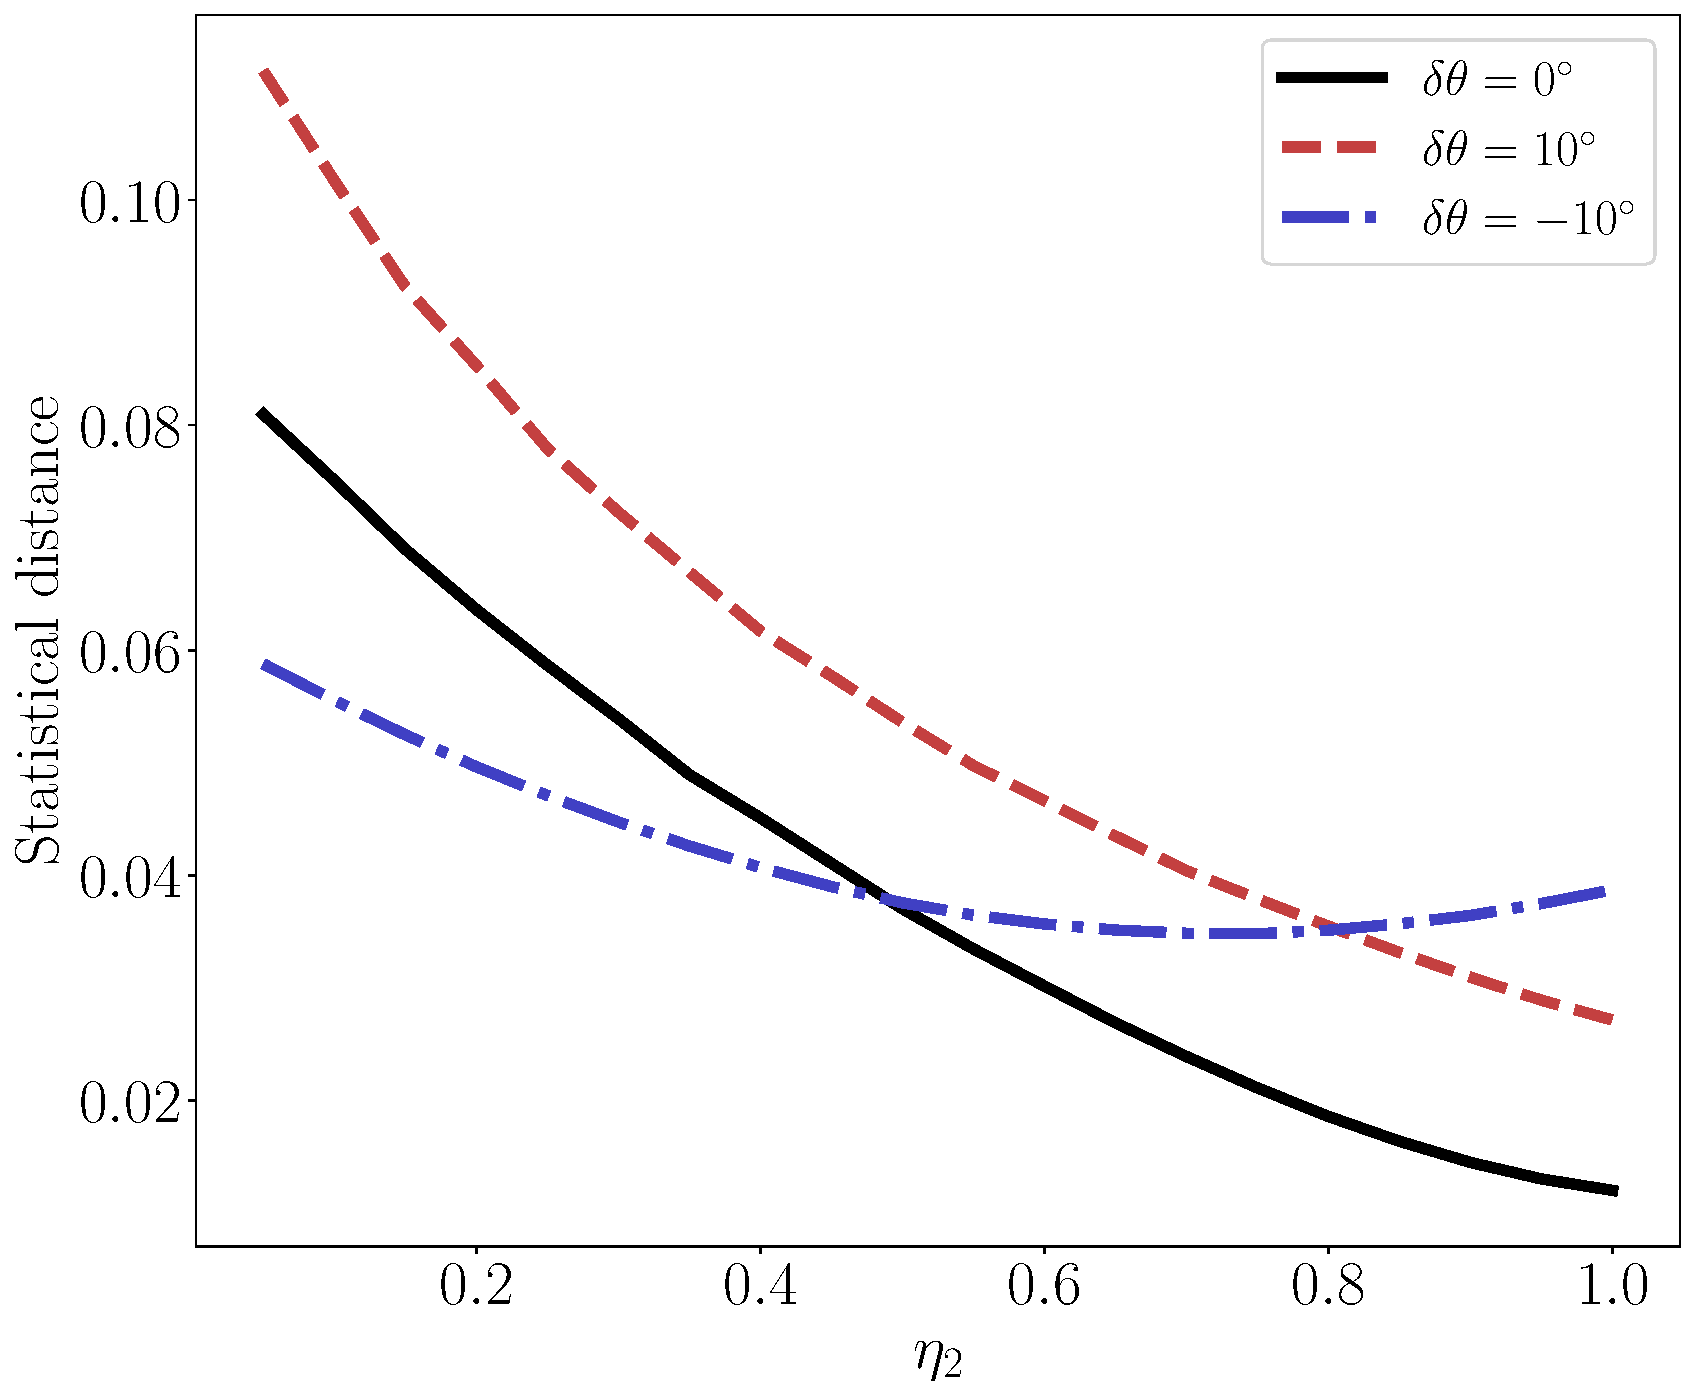
\includegraphics[width=\linewidth]{pics/homodyne/ed(eta2).pdf}
\caption[]{$\eta_1=1$}
\label{fig:eta1-1}
        \end{subfigure}
\begin{subfigure}[]{.45\linewidth}
 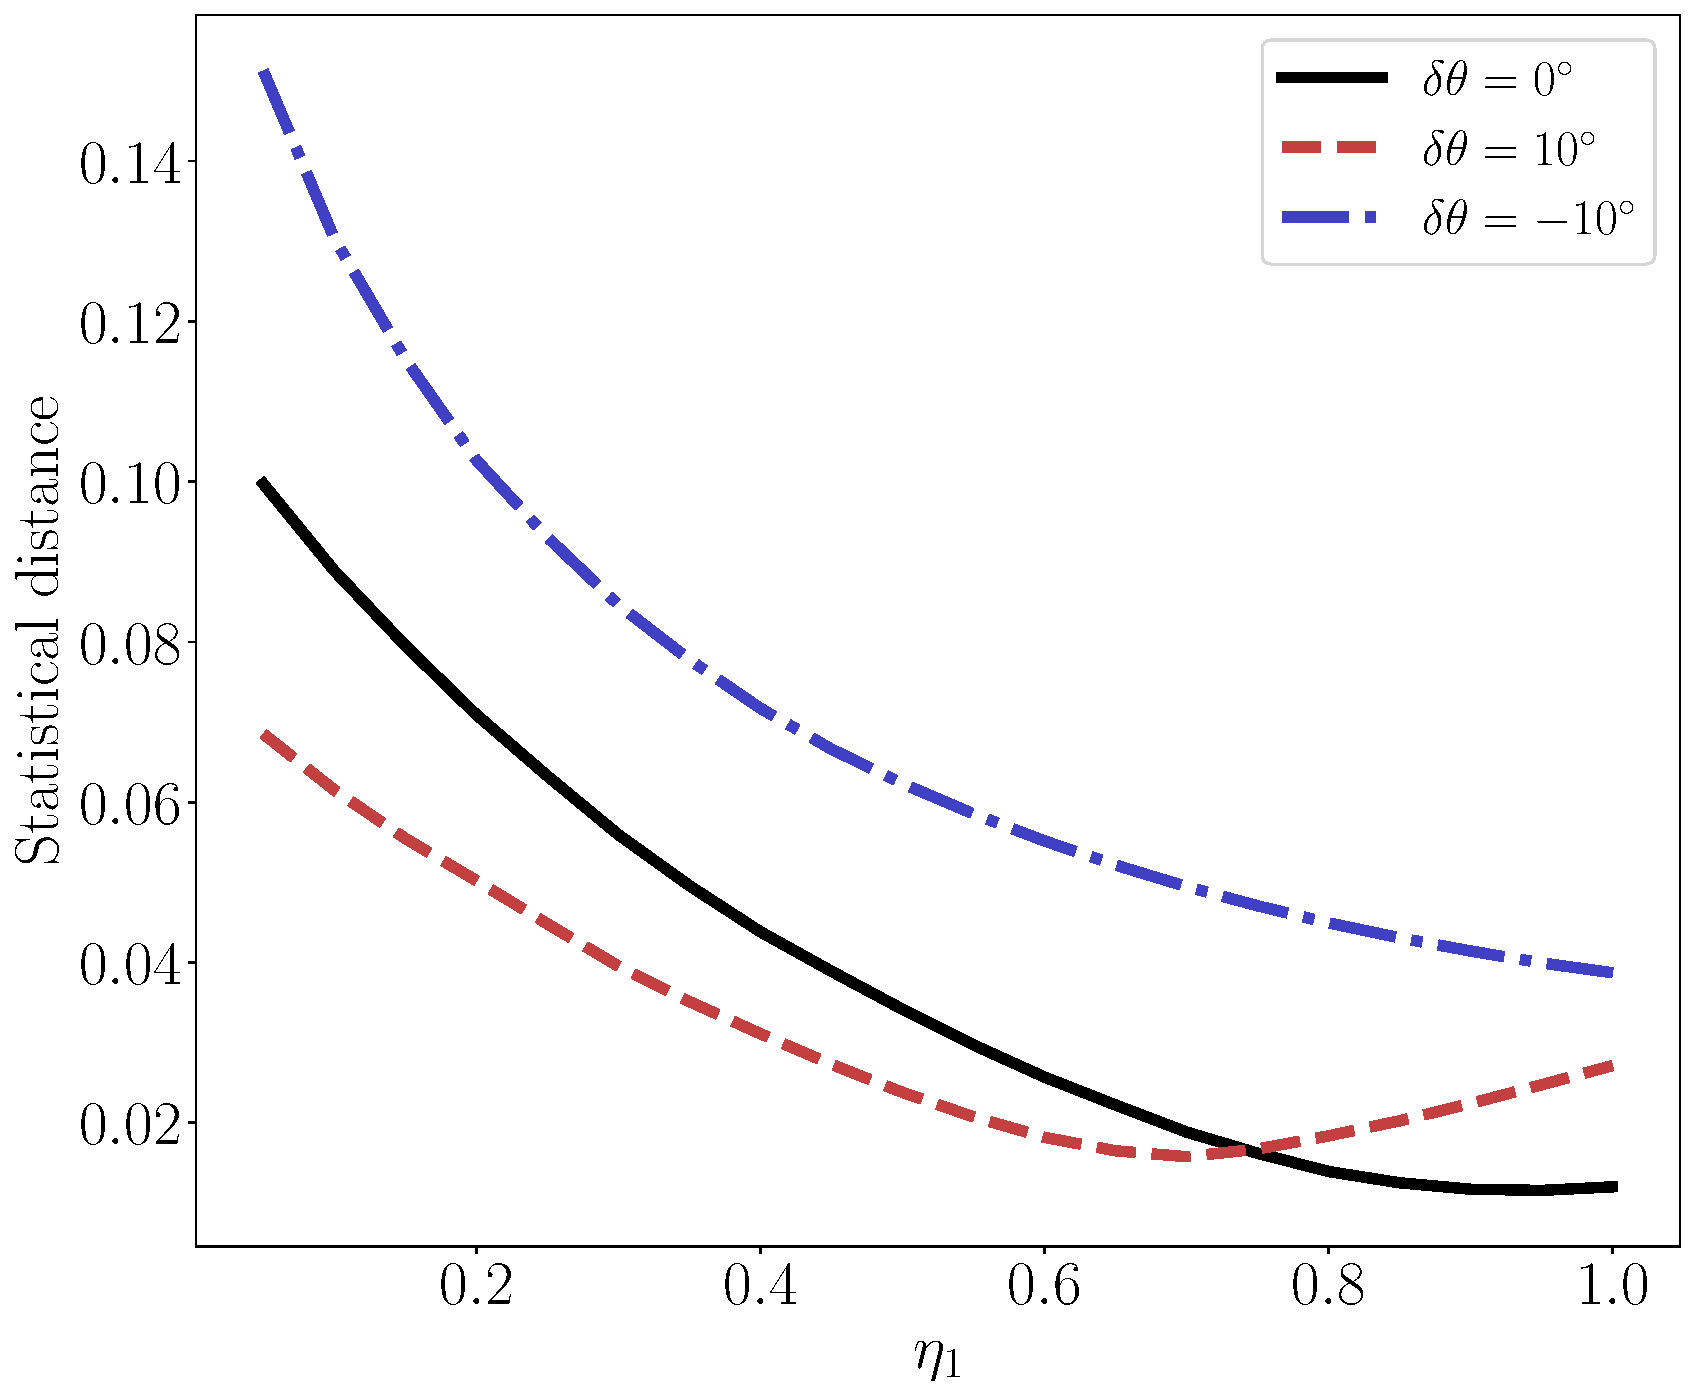
\includegraphics[width=\linewidth]{pics/homodyne/ed(eta1).pdf}
 \caption[]{$\eta_2=1$}
 \label{fig:eta2-1}
\end{subfigure}
\caption{Statistical distance $D_P=\mathtt{D}(\prob,\prob_G)$
  as a function of  photodetector efficiency
  (a)~$\eta_2$ at $\eta_1=1$ and
  (b)~$\eta_1$ at $\eta_2=1$
  for different values of the beam splitter disbalance angle
  $\delta\theta$ (see eq.~\eqref{eq:delta-theta}).
  The amplitudes are
  $|\alpha|=1$ and $|\alpha_L|=5$.
}
\label{fig:delta-eta}
\end{figure*}


In this section, we
begin with the case where the signal mode is in the coherent state
$\ket{\alpha}$ and
compare the exact statistics of difference events
governed by the Skellam distribution~\eqref{eq:accurate}
and the Gaussian approximation~\eqref{eq:Gaussian}.
In order to quantify the statistical distance between the probability distributions,
we shall use
the total variational distance
that can be computed as half of  the $L^1$ distance
\begin{align}
  &
    \label{eq:stat-dist}
    D_P\equiv\mathtt{D}\left(\prob,\prob_{G}\right)\equiv
    \frac{1}{2}
    \sum_{\mu=-\infty}^{\infty}
    \lvert\prob(\mu) -\prob_G(\mu)\rvert.
  \end{align}

  Note that, according to Eq.~\eqref{eq:stat-dist},
  $\mu$ takes integer values and
  we evaluate the distance between the probability mass fuctions,
  whereas the normalization condition for
the Gaussian function~\eqref{eq:Gaussian}
\begin{align}
    \label{eq:norm-cont}
  \int_{-\infty}^{\infty}
    \prob_G(\mu)
  \dd\mu
    =1
\end{align}
implies applicability of the continuum limit.
For integer $\mu$,
the integral
on the left hand side of Eq.~\eqref{eq:norm-cont}
should be replaced with a sum
and we have the relation
\begin{align}
  \label{eq:discr-norm}
  \sum_{\mu=-\infty}^{\infty} \prob_G(\mu)=\vartheta_3(\pi\mu_G,e^{-2\pi^2\sigma_G})\equiv N_G
\end{align}
where $\vartheta_3$ is the Jacobi elliptic theta function~\cite{NIST:hndbk:2010}.

In the applicability region of
the continuum limit, the normalization constant $N_G$
is close to unity. The numerical analysis shows that
$|N_G-1|\le 10^{-4}$ at $ 2\sigma_{G}\ge 1$.
The latter gives the condition for the LO amplitude
\begin{equation}
    |\alpha_L|\geq \frac{1}{\sqrt{2(\eta_1S^2+\eta_2C^2)}}\equiv\alpha_N
    \label{eq:renorm}
  \end{equation}
   which ensures both applicability of the continuum limit
  and proper normalization of the Gaussian approximation.
  In our calculations,
the probability $\prob_G$ will be numerically corrected by introducing
the factor $N_G^{-1}$
provided that $|\alpha_L|$ is below the "renormalization point" $\alpha_N$.


  The curves presented in Fig.~\ref{fig:amplitude}
  illustrate how the accuracy of the Gaussian approximation
  is affected by the signal and LO amplitudes, $|\alpha|$ and $|\alpha_L|$.
  More specifically, in
Fig.~\ref{fig:amp_05} (Fig.~\ref{fig:amp_01}),
  the statistical distance is numerically evaluated as a function
  of the amplitude $|\alpha|$ ($|\alpha_L|$)
at different values of the photodetectors efficiencies
provided that the value of
the other amplitude $|\alpha_L|$ ($|\alpha|$) is fixed.

\begin{figure*}
    \centering
    \begin{subfigure}[]{.45\textwidth}
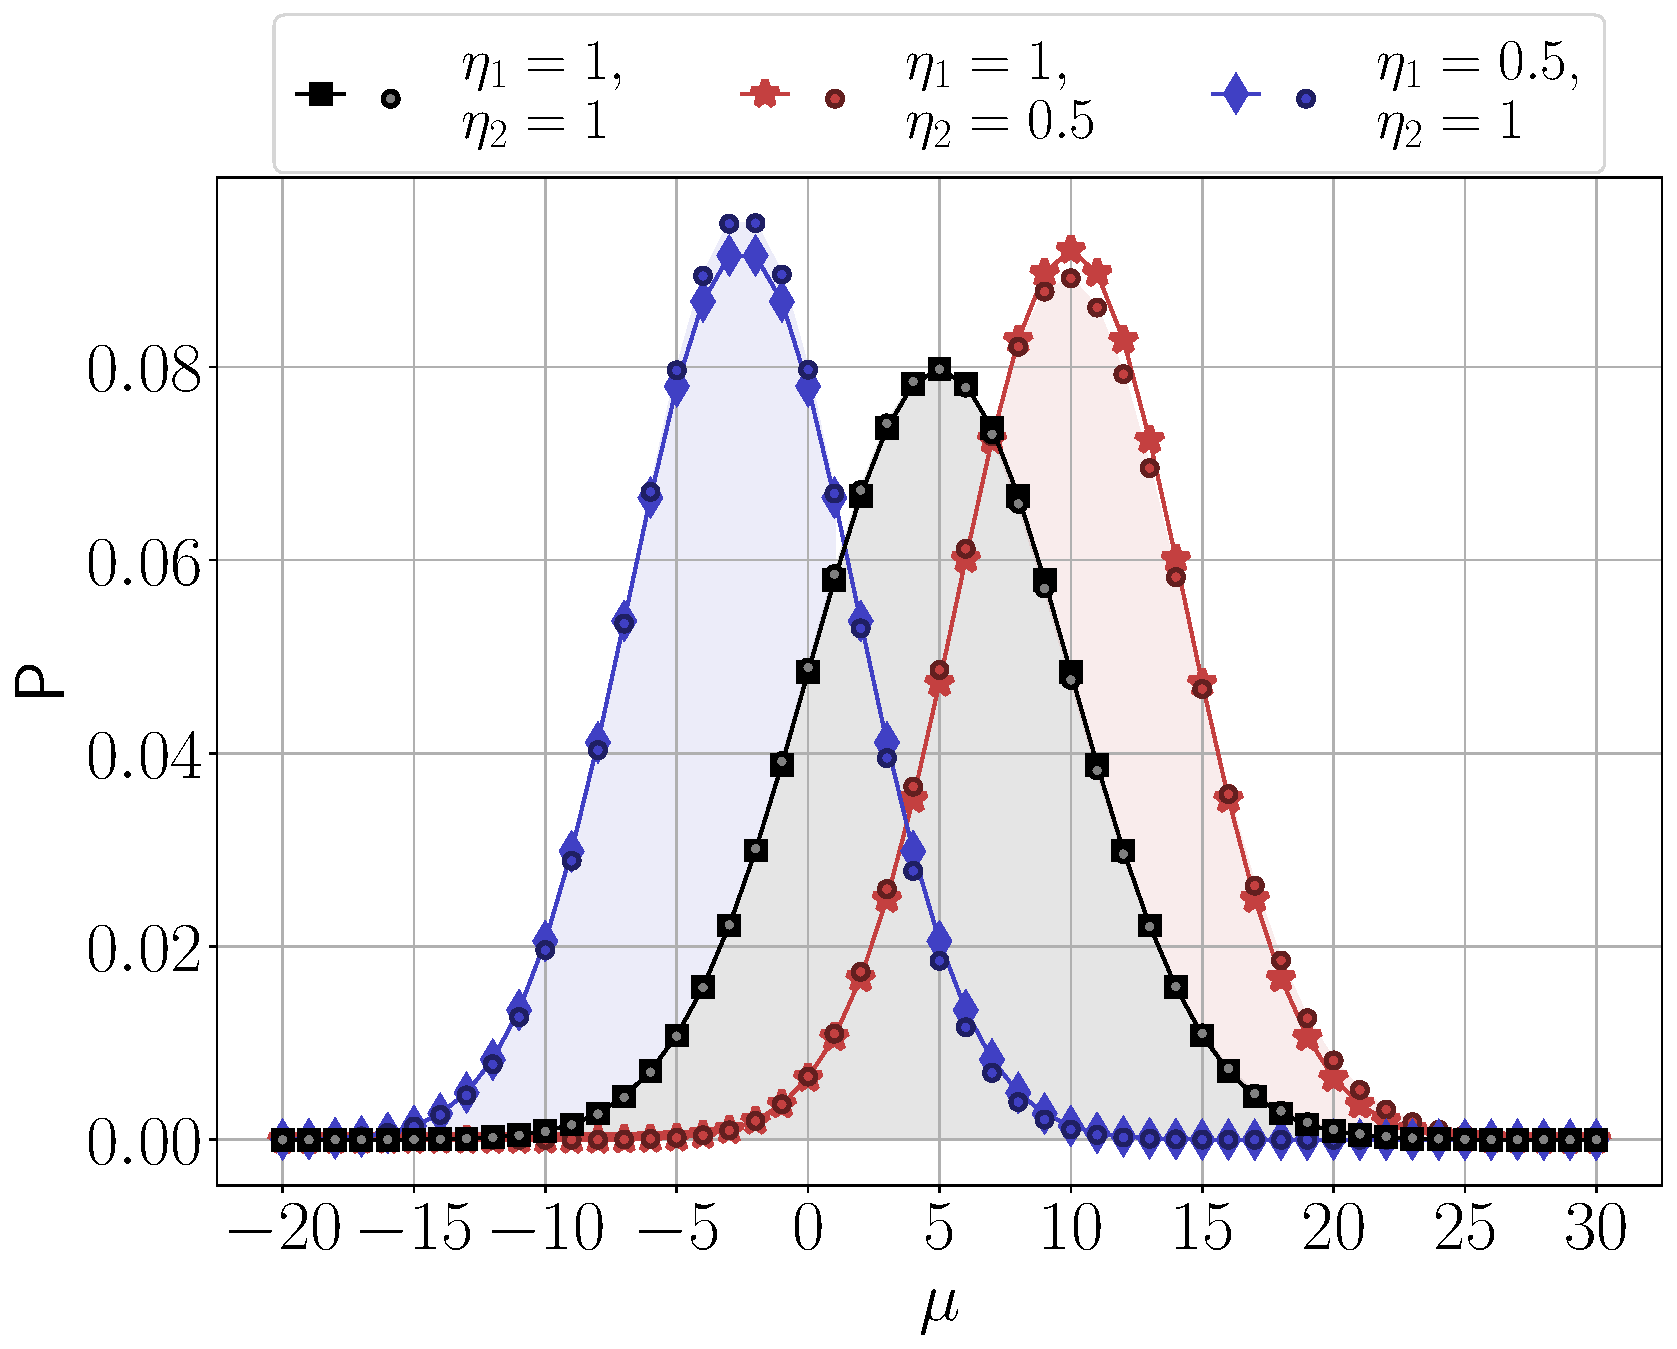
\includegraphics[width=\linewidth]{pics/homodyne/coherent_distributions.pdf}
\caption[]{$\ket{\psi}=\ket{\alpha},\:$$\alpha=0.5$}
\label{fig:dist_alp}
        \end{subfigure}
        \begin{subfigure}[]{.45\textwidth}
 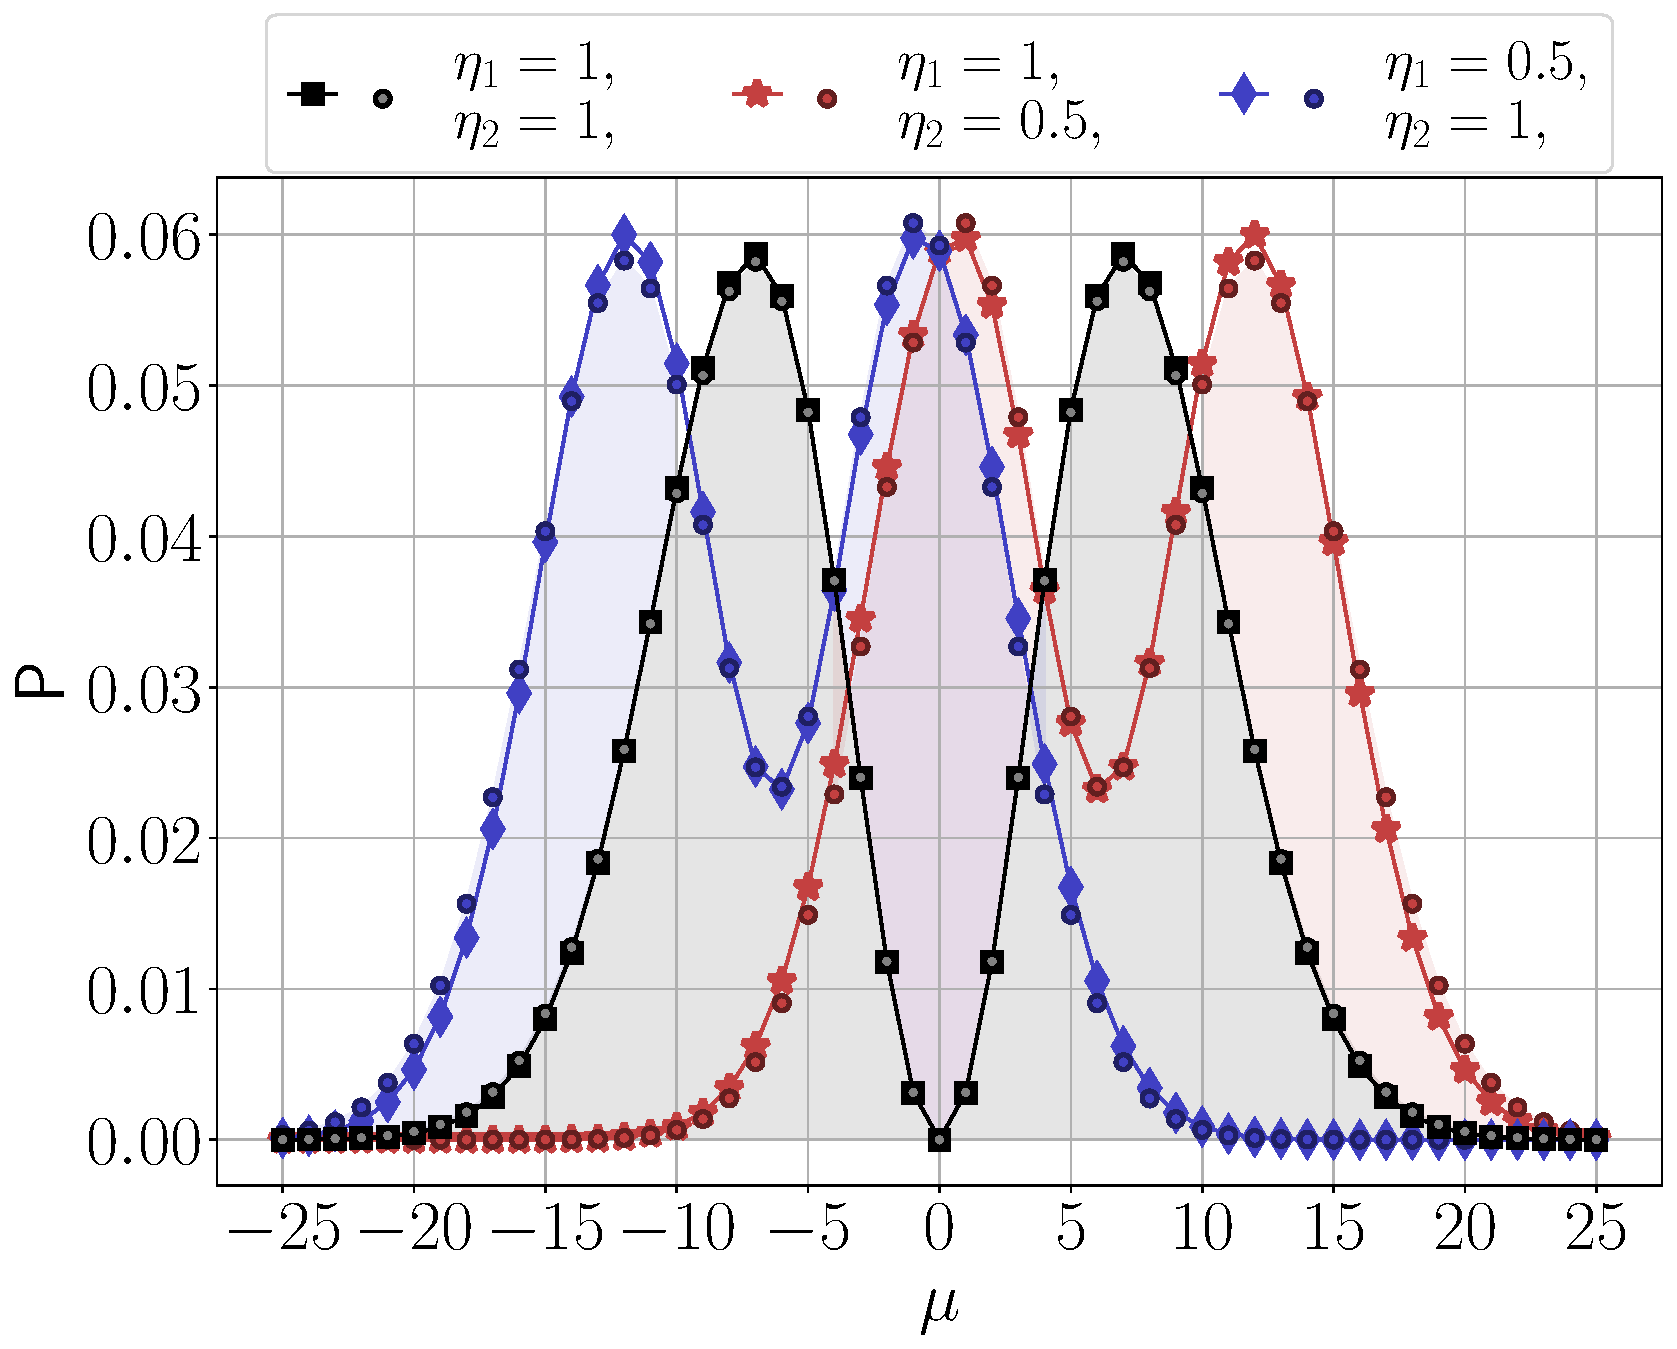
\includegraphics[width=\linewidth]{pics/homodyne/fock_distributions.pdf}
\caption[]{$\ket{\psi}=\ket{n},\:n=1$}
\label{fig:dist_fock}
\end{subfigure}
\caption{Statistical distributions of photon count difference
  for the signal mode prepared in (a)~the coherent state and
  in (b)~the single photon Fock state computed for
  for different efficiencies  at $|\alpha_L|=5$
  and $\delta\theta=0$.
}
\label{fig:dist-hom}
\end{figure*}


\begin{figure*}
    \centering
    \begin{subfigure}[]{.45\textwidth}
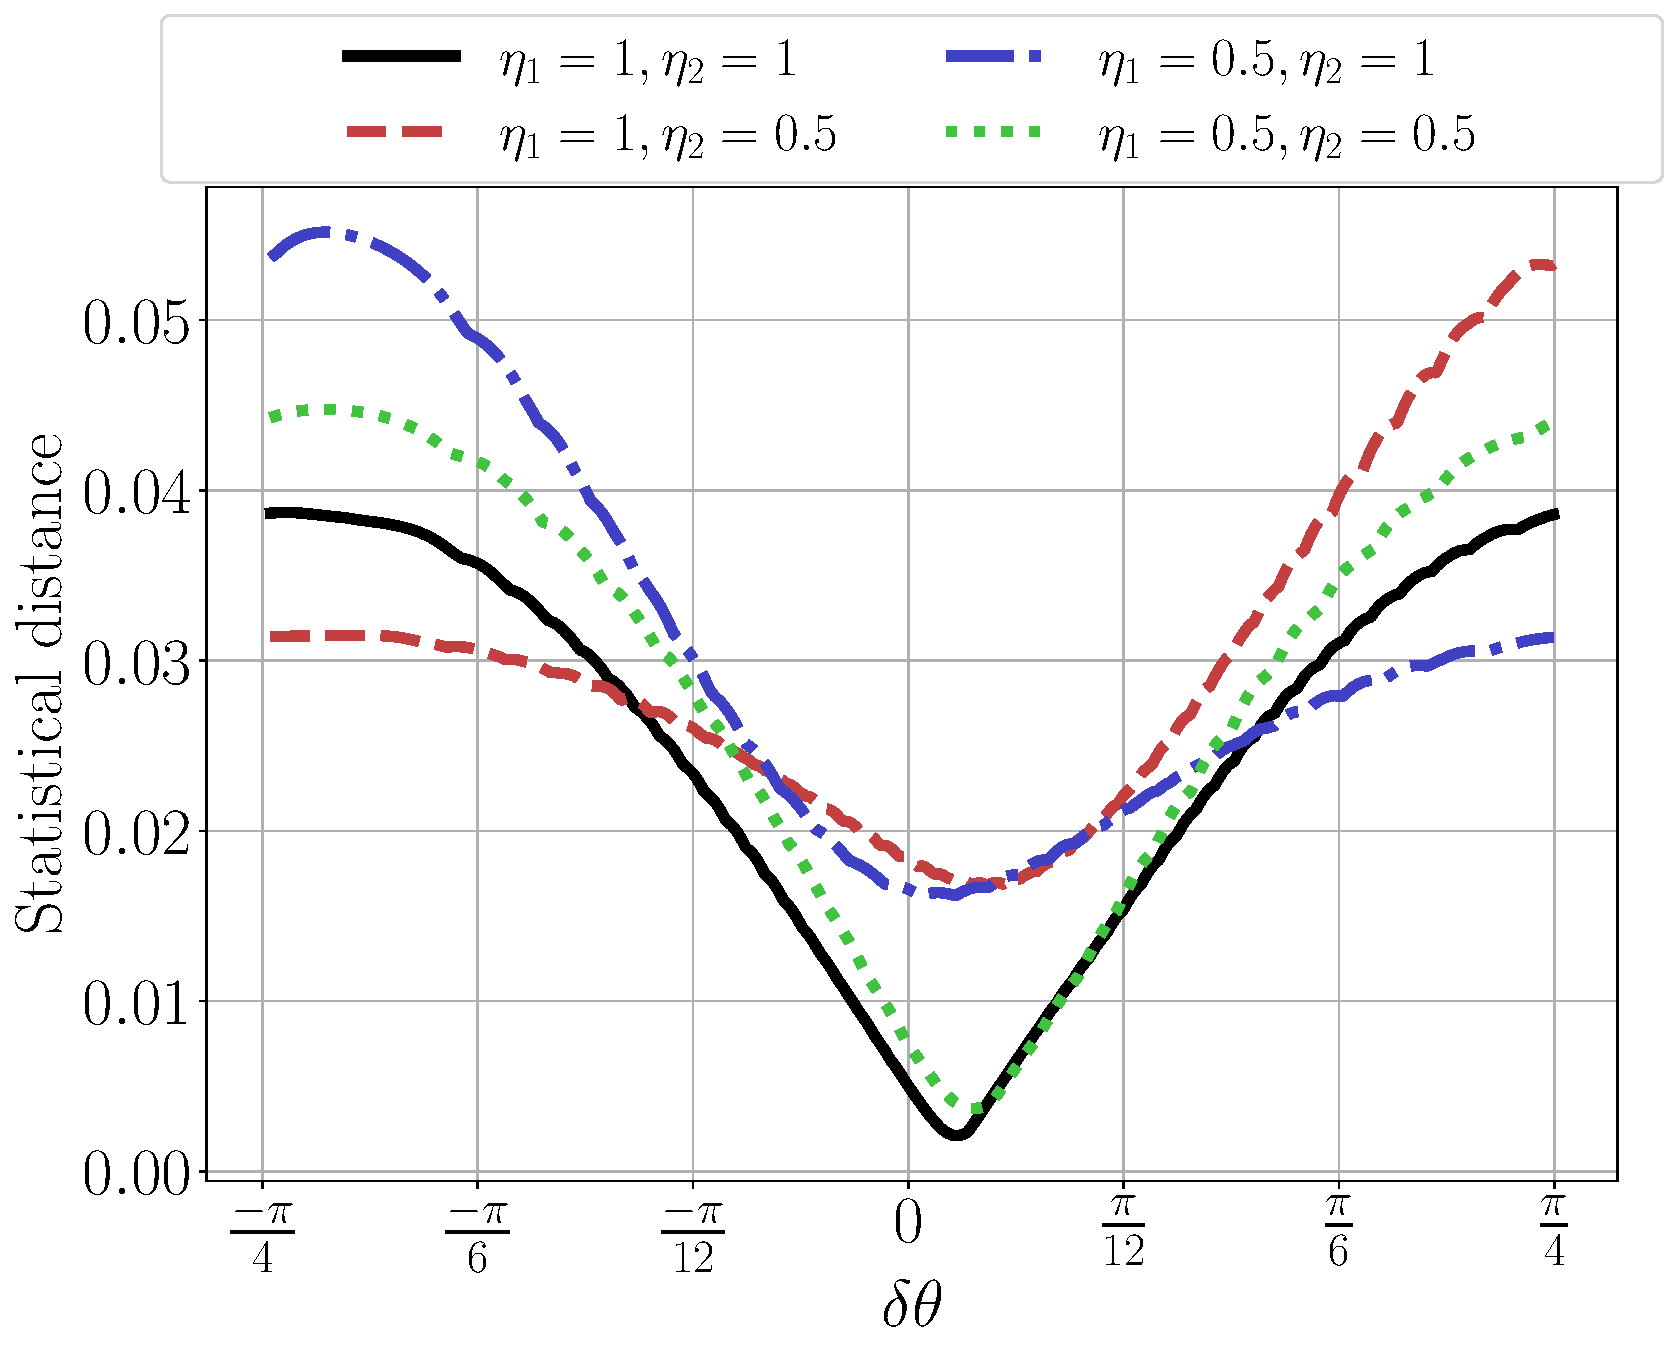
\includegraphics[width=\linewidth]{pics/homodyne/full.pdf}
\caption[]{$\ket{\psi}=\ket{\alpha},\:\alpha=0.5$}
\label{fig:dth_alp}
        \end{subfigure}
        \begin{subfigure}[]{.45\textwidth}
 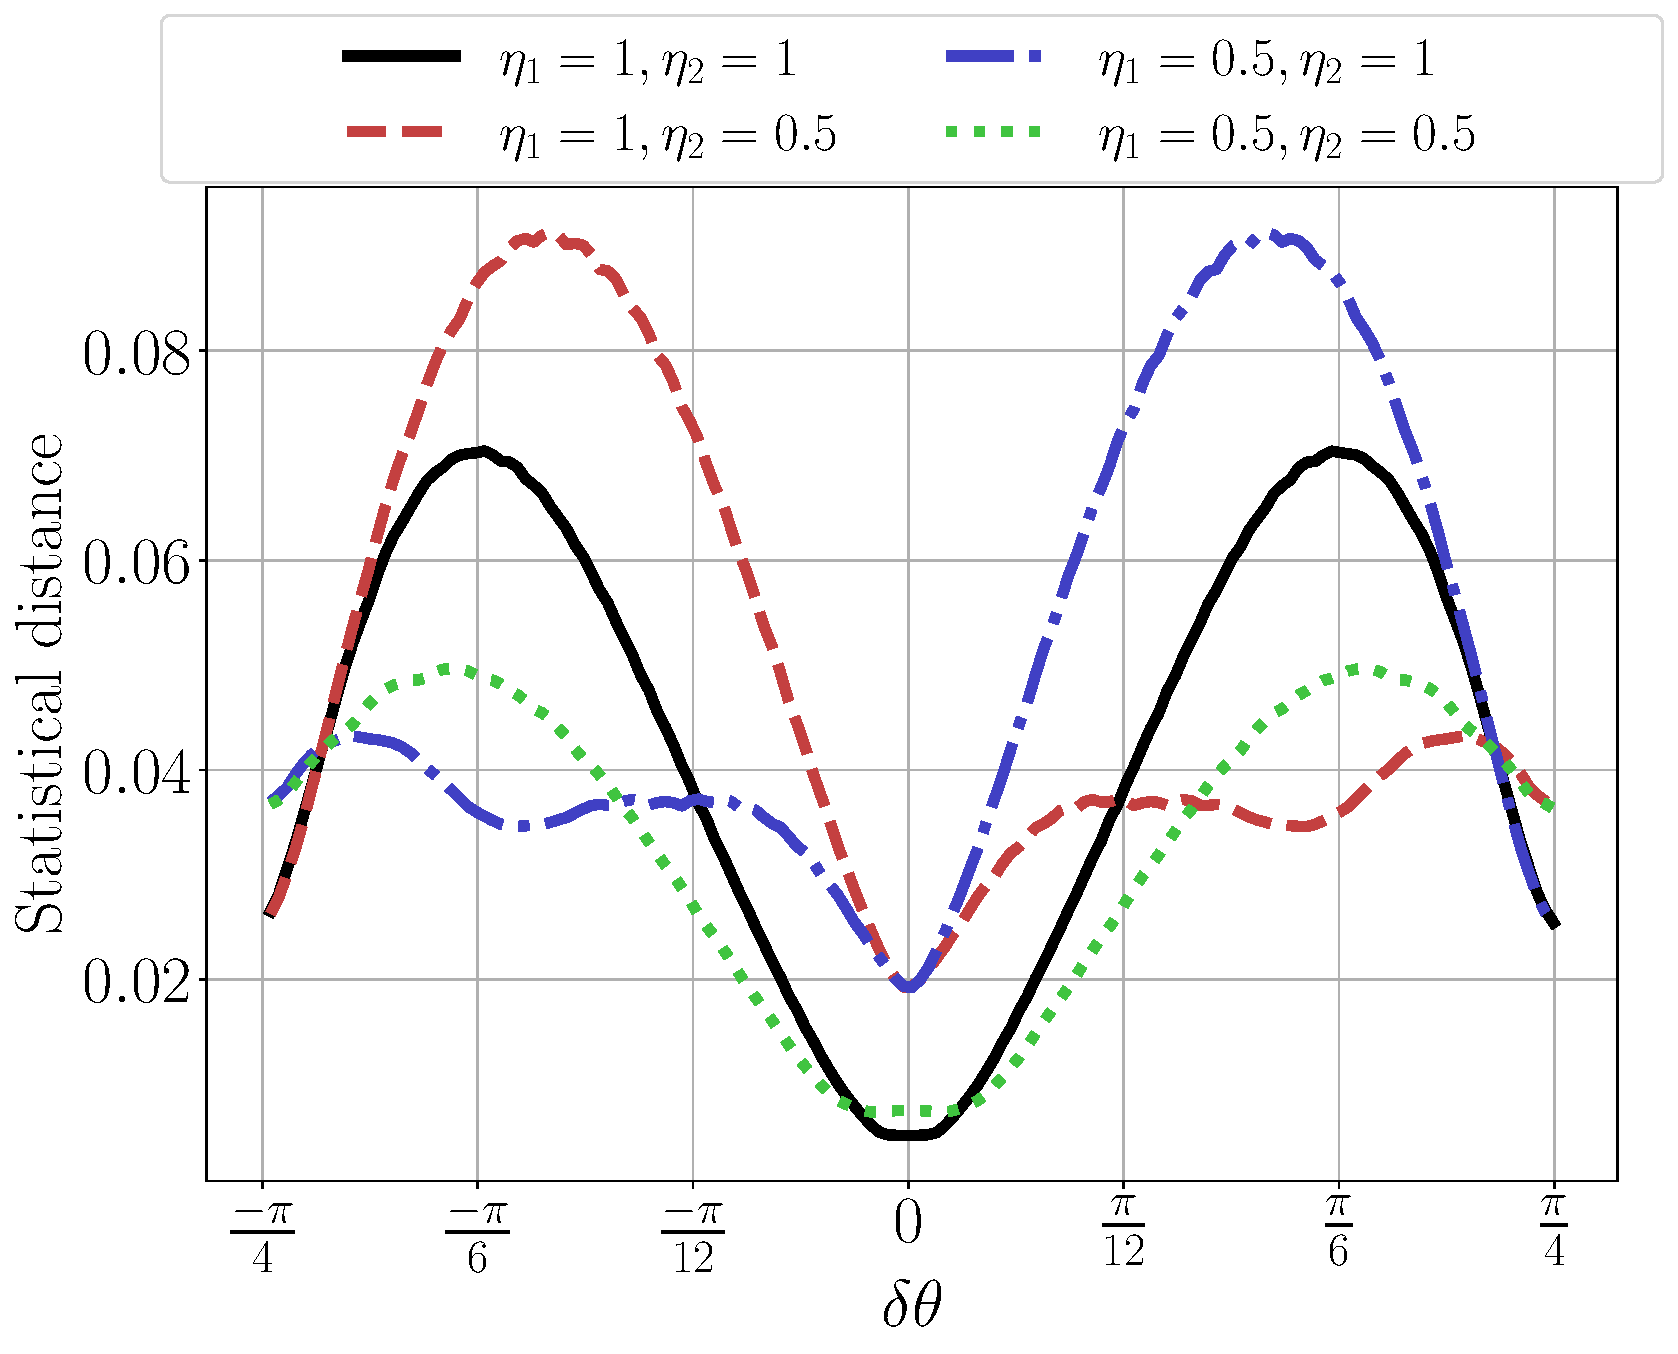
\includegraphics[width=\linewidth]{pics/homodyne/full_fock.pdf}
\caption[]{$\ket{\psi}=\ket{n},\:n=1$}
\label{fig:dth_fock}
\end{subfigure}
\caption{
  Statistical distance $D_P=\mathtt{D}(\prob,\prob_G)$
  as a function of the beam splitter disbalance angle, $\delta\theta$,
for the signal mode prepared in (a)~the coherent state and
  in (b)~the single photon Fock state at different efficiencies  with $|\alpha_L|=5$.
    }
    \label{fig:delta-theta}
\end{figure*}


Referring to Fig.~\ref{fig:amp_05},
the curves behave as expected:
given the LO amplitude $|\alpha_L|$,
the distance monotonically increases with $|\alpha|$.
It is shown that,
at $|\alpha_L|=5$ and $|\alpha|>1$,
the perfectly symmetric homodyne presents the case
with minimal distance, $D_P$, while in the presence of asymmetry,
the curves exhibit a rapid growth and
the quality of  the Gaussian approximation
rapidly degrades to the point, where $D_P>0.1$,
so it is not useful for its intended purpose.

When it comes to dependencies of the statistical distance on
the LO oscillator amplitude
computed at fixed value of $|\alpha|$,
the above results suggest that the smaller the amplitude $|\alpha|$
the better the accuracy of the Gaussian approximation.
We can also expect the distance
will be small provided that $|\alpha_L|$ is large
and the strong LO approximation is applicable. 


Referring to Fig.~\ref{fig:amp_01},
the curves evaluated at $|\alpha|=0.5$
display a non-monotonic behavior with two local maxima
in the weak LO range where $|\alpha_L|<1$.
By contrast, after the second maximum at $|\alpha_L|>1$,
the distance falls with the LO amplitude
and it drops below $0.05$ at $|\alpha_L|>2$.

Note, that, when $|\alpha|<0.1$
and the signal mode state is close to the vacuum state,
the two local maxima of $D_P$ can be estimated to be slightly above $0.08$ and $0.1$,
respectively. So, in this case, the distribution~\eqref{eq:Gaussian}
might be regarded as a reasonable approximation even in the
weak LO range where
the probability $\prob_G$ approaches the close neighborhood of
the singular limit,
$\lim_{|\alpha_L|\to 0}\prob_G(\mu)=\delta(\mu)$. 


From Fig.~\ref{fig:amp_01},
it can also be seen that
the distance vs LO amplitude dependence
that can be used as a tool to characterize
the applicability region of the strong LO approximation
is nearly insensitive to asymmetry.
In other words, the latter does not produce noticeable effects on
the accuracy of the approximation.


The parameters describing
the photodetection asymmetry are
the efficiencies $\eta_1$ and $\eta_2$.
The curves plotted in Fig.~\ref{fig:amplitude}
are computed at different values of the efficiencies.

In order to quantify deviation of the beam splitter
transmission and reflection amplitudes
from the balanced $50:50$ values
$t=\cos\theta=r=\sin\theta=1/\sqrt{2}$ at
the angle $\theta=\pi/4$,
we introduce the beam splitter \textit{disbalance angle} given by
\begin{equation}
  \label{eq:delta-theta}
        \delta\theta\equiv\frac{\pi}{4}-\theta.
      \end{equation}

      In Figure~\ref{fig:delta-eta}
      we plot the distance against
      the efficiency of the photodetector assuming that the
      other photodetector is perfect.
      The curves are evaluated at different values of the
      disbalance angle~\eqref{eq:delta-theta}.
The efficiency dependence of
the distance
is shown to decrease monotonically at $\delta\theta=0$.
In contrast, for disbalanced beam splitter, this dependence can
reveal non-motonic behavior.

So far, we have used the analytical results
obtained in Sec.~\ref{subsec:gauss-hom}
for the case where the LO and signal modes are both
in the coherent states.
In the general case when the quantum state of the signal mode
is $\ket{\psi}$,
the probability distributions can be evaluated
using the relations
\begin{align}
  &
\label{eq:average-P-func}
    \prob(\mu;\ket{\psi})=\int  P_{\ket{\psi}}(\alpha)\prob(\mu;\alpha)\dd^2\alpha,
    \notag
  \\
  &
    \prob_G(x;\ket{\psi})=\bra{\psi}\hat{\Pi}_G\ket{\psi},
\end{align}
where $P_{\ket{\psi}}(\alpha)$ is the Glauber $P$ function of the quantum state
$\ket{\psi}$.
In Figs.~\ref{fig:dist-hom}
and~\ref{fig:delta-theta},
we show the results computed for the single-photon Fock states
obtained utilizing
the well-known expression for
the $P$-function of Fock states $\ket{\psi}=\ket{n}$ given by
%\cite{vogel2006quantum}
\begin{equation}
\label{eq:P-function_fock}
P_{\ket{n}}(\alpha)=
\frac{e^{|\alpha|^2}}{n!}
\Bigl(
\frac{\partial^2}{\partial\alpha\partial\cnj{\alpha}}
\Bigr)^n
\delta^{2}(\alpha),
\end{equation}
where $\delta^{2}(\alpha)=\delta(\Re\alpha)\delta(\Im\alpha)$.

Figure~\ref{fig:dist-hom} displays
the photocount difference probabilities
computed from
the exact and Gaussian probability distributions
for the balanced beam splitter at different photodetector efficiencies
and signal mode input states.
From Fig.~\ref{fig:dist_alp},
it is seen that,
in agreement with Eq.~\eqref{eq:mu_G},
asymmetry in photodetection
results in the shift of the probability maximum.
Note that, at $\delta\theta=0$,
the photocount variance~\eqref{eq:sigma_G},
$\sigma_G=(\eta_1+\eta_2)|\alpha_L|^2/2$, and
the quadrature variance~\eqref{eq:sigma-x},
$\sigma_x=2/(\eta_1+\eta_2)$,
are both invariant under transposition of the photodetectors:
$\eta_{1}\leftrightarrow \eta_{2}$.

The distributions for the single-photon states
are depicted in Fig.~\ref{fig:dist_fock}
and, similar to the coherent state,
demonstrate the effect of asymmetry-induced shift.
Another noticeable effect is that
the probability minima between the central and side peaks
become less pronounced.

The photodetector efficiencies
and the signal mode input states
of Fig.~\ref{fig:dist-hom}
are used to compute
the statistical distance vs disbalance angle
curves presented in Fig.~\ref{fig:delta-theta}.
These curves illustrate how the beam splitter disbalance and
the photodetector efficiencies influence the accuracy of the
Gaussian approximation.
The distance is shown to be minimal in the vicinity of
the balanced beam splitter point with
a vanishing disbalance angle, $\delta\theta=0$.

  

\begin{figure}
    \centering
    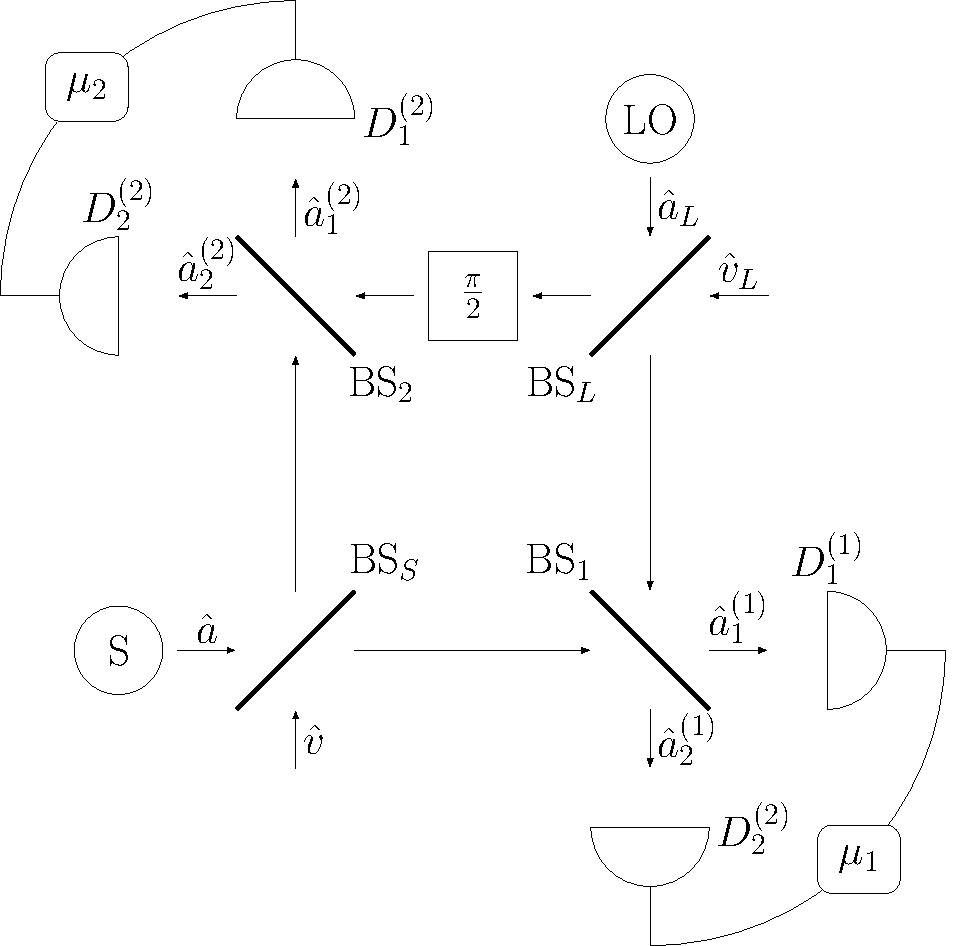
\includegraphics[width=0.9\linewidth]{pics/schemes/double_homodyne.pdf}
    \caption{Scheme of an eight port double homodyne receiver.
      S is the source of the signal mode
      $\hat{a}$; LO is the source of the reference mode $\hat{a}_{L}$;
      BS$_S$ (BS$_L$) is the signal mode (local oscillator) beam splitter;
      $\frac{\pi}{2}$ is the quarter wave phase shifter;
BS$_i$ is the beam splitter of $i$th homodyne;
$D_{1,2}^{(i)}$ are the photodetectors of the $i$th homodyne;
and $\mu_i=m_1^{(i)}-m_2^{(i)}$ is the photon count difference registered by
the detectors of $i$th homodyne.
    }
    \label{fig:double-homodyne}
\end{figure}



%%%%%%%%%%%%%%%%%%%%%%%%%%%%%%%%%%%%%%%
% \section{Discussion}
% \label{sec:discussion}
%%%%%%%%%%%%%%%%%%%%%%%%%%%%%%%%%%%%%%%%

%\section{Double homodyne detection scheme}\label{sec-double-homodyne}

Consider the 8-port double homodyne scheme (Fig.~\ref{fig:double-homodyne}) \cite{lahti2010realistic}. It is known that this measurement scheme allows to reconstruct the $Q$-function of the signal state \cite{Richter:98}, yielding full information about the signal state, which may be used in CV-QKD protocols. It should be noted that the restoration of the state complex amplitude entirely serves as the basis for composable security proofs~\cite{PhysRevLett.93.170504,PhysRevLett.118.200501,pirandola2024improvedcomposablekeyrates,pascualgarcía2024improvedfinitesizekeyrates}. Analogous to Eq.~\eqref{eq:accurate}, the statistical distribution of photon count difference is written as:
\begin{multline}
P= \left(\frac{\eta_1|\alpha_1|^2}{\eta_4|\alpha_4|^2}\right)^{\frac{\delta m_1}{2}}
I_{\delta m_1}\left(2\sqrt{\eta_1\eta_4|\alpha_ 1|^2|\alpha_4|^2}\right)
e^{-\eta_1|\alpha_1|^2}
e^{-\eta_4|\alpha_4|^2}\times\\\times
\left(\frac{\eta_3|\alpha_3|^2}{\eta_2|\alpha_2|^2}\right)^{\frac{\delta m_2}{2}}
I_{\delta m_2}\left(2\sqrt{\eta_2\eta_3|\alpha_ 2|^2|\alpha_3|^2}\right)
e^{-\eta_2|\alpha_2|^2}
e^{-\eta_3|\alpha_3|^2}\label{eq:accurate-dh},
\end{multline}
where
\begin{align}
\begin{split}
    |\alpha_1|&=|
    C_1C_2\alpha
    -S_3S_2\alpha_L|,\\
    |\alpha_2|&=
    |S_1C_4\alpha
    -iC_3S_4\alpha_L|,\\
    |\alpha_3|&=|
     S_1S_4\alpha
    +iC_3C_4\alpha_L|,\\
    |\alpha_4|&=|
    C_1S_2\alpha+
    S_3C_2\alpha_L|.
\end{split}
\end{align}

The approximation method used in the previous section yields the Gaussian approximation
\begin{multline}
P_G=\frac{\biggl[(\eta_1S_2^2+\eta_4C_2^2)(\eta_3C_4^2+\eta_2S_4^2)\biggr]^{-\frac{1}{2}}}{2\pi C_3S_3|\alpha_L|^2}\times\\\times \exp \biggl[-D_1\left(x_1+\frac{\Re\alpha\alpha_L^*}{|\alpha_L|}\right)^2\biggr]\exp \biggl[-D_2\biggl(x_2-\frac{\Im\alpha\alpha_L^*}{|\alpha_L|}\biggr)^2\biggr], \label{eq:Pgood-dh}
\end{multline}
where designations
\begin{align}
    \begin{split}
D_1&=\frac{2(C_1C_2S_2[\eta_1+\eta_4])^{2}}{\eta_1S_2^2+\eta_4C_2^2},\\
    D_2&=\frac{2(S_3S_4C_4[\eta_3+\eta_2])^2}{\eta_3C_4^2+\eta_2S_4^2},
    \end{split}\label{eq:dh-D}
\end{align}
\begin{align}
    \begin{split}
x_1&=\frac{\delta m_1}{2|\alpha_L|C_1C_2S_2S_3[\eta_1+\eta_4]}+\frac{-\eta_1S_2^2S_3^2+\eta_4S_3^2C_2^2}{2C_1C_2S_2S_3[\eta_1+\eta_4]}|\alpha_L|, \\
    x_2&=\frac{\delta m_2}{2|\alpha_L|S_1S_4C_3C_4[\eta_3+\eta_2]}+\frac{-\eta_3C_3^2C_4^2+\eta_2C_3^2S_4^2}{2S_1S_4C_3C_4[\eta_3+\eta_2]}|\alpha_L|
    .
    \end{split}\label{eq:dh-x}
\end{align}
have been introduced. Note that Eq.~\eqref{eq:Pgood-dh} is a product of two functions in the form of Eq.~\eqref{eq:Pgood} (much like Eq.~\eqref{eq:accurate-dh} is a product of two function in the form of Eq.~\eqref{eq:accurate}), meaning approximation quality study in previous section fully applies for this case. Indeed, the difference statistics of the double homodyne scheme is difference statistics of two separate homodyne schemes with quadrature displaced by $\frac{\pi}{2}$, normalized to unity (See Fig.~\ref{fig:dh-statistics}). 

Using the method introduced in the previous section, by comparing Eq.\eqref{eq:Pgood-dh} of the ideal scheme and the $Q$-function of coherent state,
\begin{equation}
    |\langle\beta|\alpha\rangle|^2=\exp\left[-
    (\beta_1-\alpha_1)^2-(\beta_2-\alpha_2)^2
    \right], %ez 2 show
\end{equation}
where for complex numbers we introduced the notation $\alpha=\alpha_1+i\alpha_2$, and introducing 
\begin{align}
\begin{split}
    \sigma_{D_1}\equiv\frac{1}{D_1}-1,\\
    \sigma_{D_2}\equiv\frac{1}{D_2}-1,
\end{split}
\label{eq:dh-G}
\end{align}
we may write $P_G$ in the form
\begin{multline}
    {{P}}_G=\frac{1}{4{\pi}C_3S_3[\eta_1+\eta_4][\eta_3+\eta_2]S_2^2\sqrt{ C_1C_2S_4C_4}|\alpha_L|^2} \int \mathop{dx'_1dx'_2}\times\\\times G(x_1-x_1', \sigma_{D_1})G(x_2-x_2', \sigma_{D_2})|\langle\alpha|e^{-i\phi_L}\left(-x_1'+ix_2'\right)\rangle|^2,%\label{eq:dh-povm}
\end{multline}
where $|e^{-i\phi_L}\left(-x_1'+ix_2'\right)\rangle$ is a coherent state. This allows us to write the respective POVM as
\begin{multline}
    \hat{{P}}_G=\frac{1}{4{\pi}C_3S_3[\eta_1+\eta_4][\eta_3+\eta_2]S_2^2\sqrt{C_1C_2S_4C_4}|\alpha_L|^2} \int \mathop{dx'_1dx'_2}\times\\\times G(x_1-x_1', D_1)G(x_2-x_2', D_2)|e^{-i\phi_L}\left(-x_1'+ix_2'\right)\rangle\langle e^{-i\phi_L}\left(-x_1'+ix_2'\right)|.\label{eq:dh-povm}
\end{multline}
Note the difference between definitions of variances of Gaussian functions Eq.~\eqref{eq:h-G} and Eq.~\eqref{eq:dh-G}, namely the difference in variances by a factor of $2$. This is due to $Q$-functions with which we compare approximations with ideal parameters having (and not having) an explicit factor of $2$ in their variances.

We may also see that $D_1$ and $D_2$, defined by Eq.~\eqref{eq:dh-D}, may be greater than $1$ for some parameters of the system. This becomes apparent once we present $D_1$ ($D_2$) as $2C_1^2D$ ($2S_3^2D$), with $D$ defined as per Eq.~\eqref{eq:defs-x-D}. This is an issue due to the variances $\sigma_{D_1}$ and $\sigma_{D_2}$ given by Eq.~\eqref{eq:dh-G}, being negative for these parameters, meaning that any asymmetry in BS$_1$ and BS$_3$ is not described by POVM given by Eq.~\eqref{eq:dh-povm}. \hl{Evidently, using coherent states for this case is flawed, see Ref.{~\cite{doi:10.1080/09500348714550131}}, where, for similar case of non-balanced BS$_{1,3}$, POVM is derived to be a projector onto squeezed coherent state.} This problem requires further investigation and is beyond the scope of this work.

\begin{figure}
    \centering
    \begin{minipage}[c]{.75\linewidth}
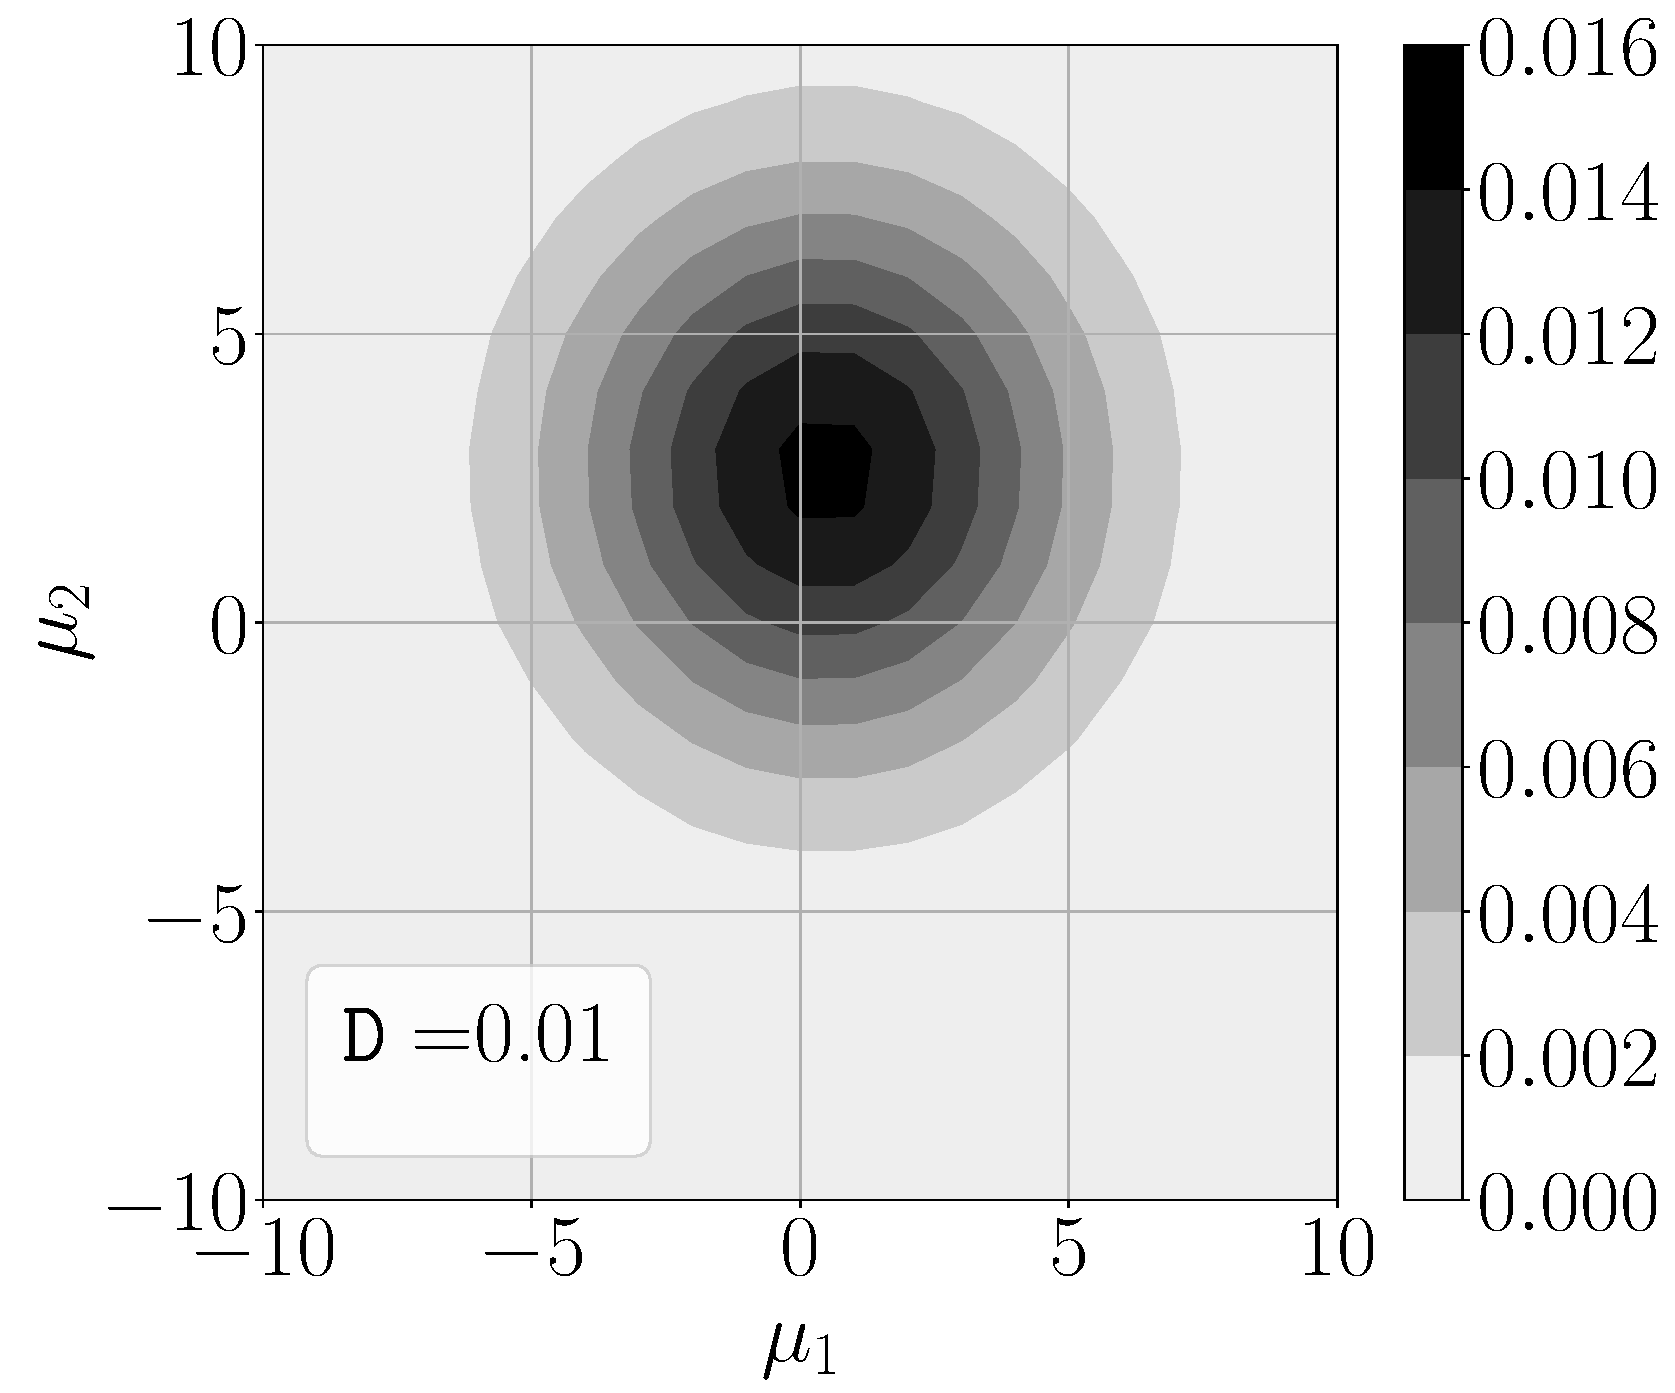
\includegraphics[width=\linewidth]{pics/double-homodyne/full.pdf}
\subcaption[]{}
        \end{minipage}
\hfill
        \begin{minipage}[c]{.45\linewidth}
 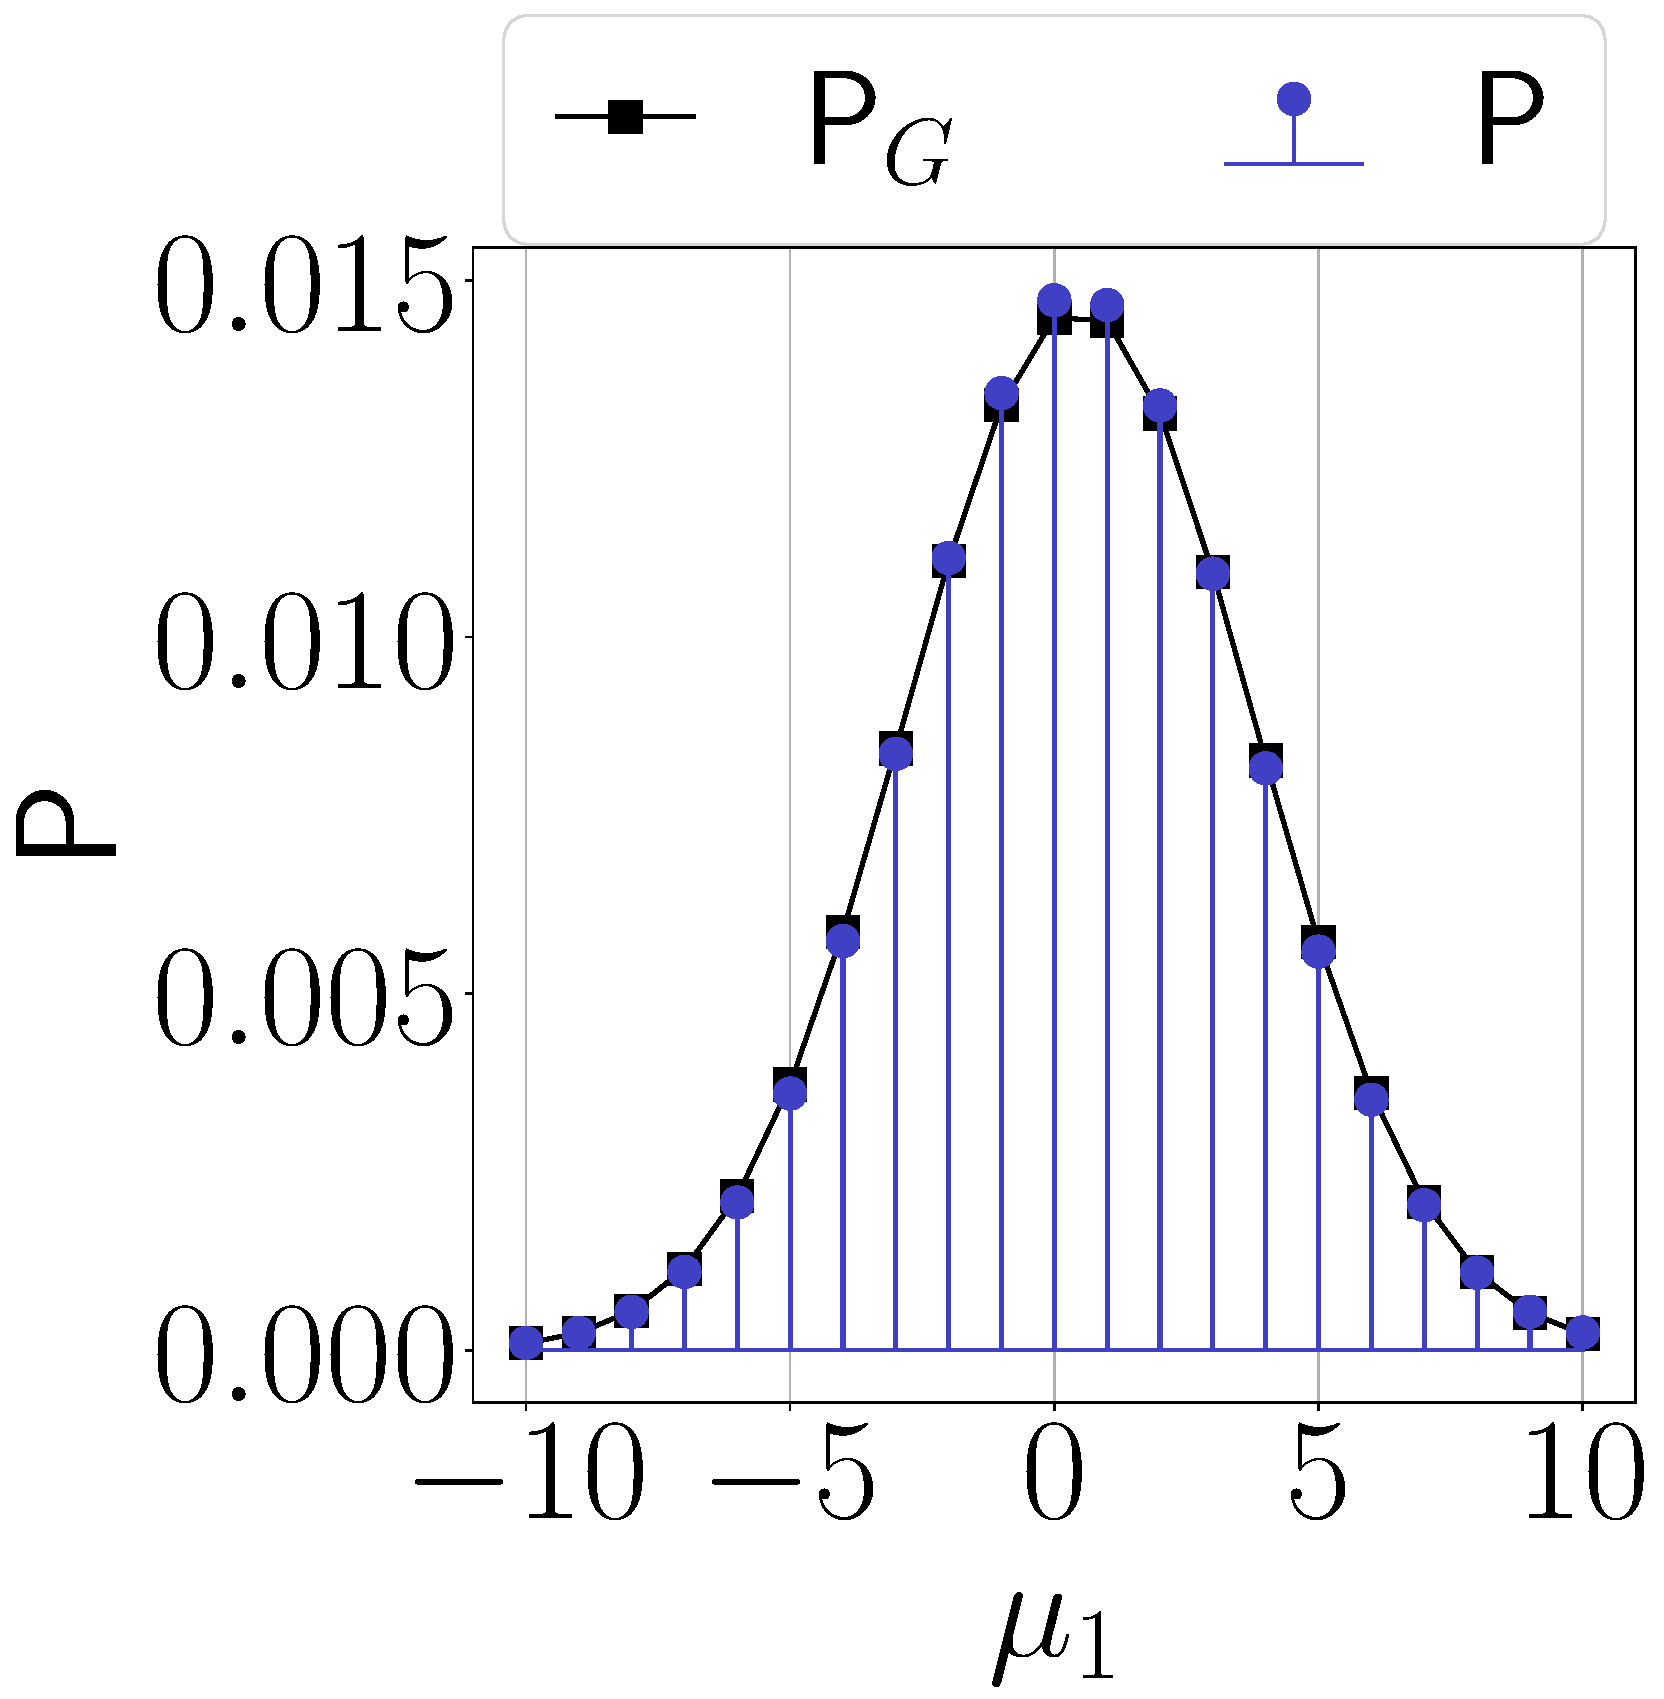
\includegraphics[width=\linewidth]{pics/double-homodyne/dm1.pdf}
\subcaption[]{}
\end{minipage}
\hfill
        \begin{minipage}[c]{.45\linewidth}
 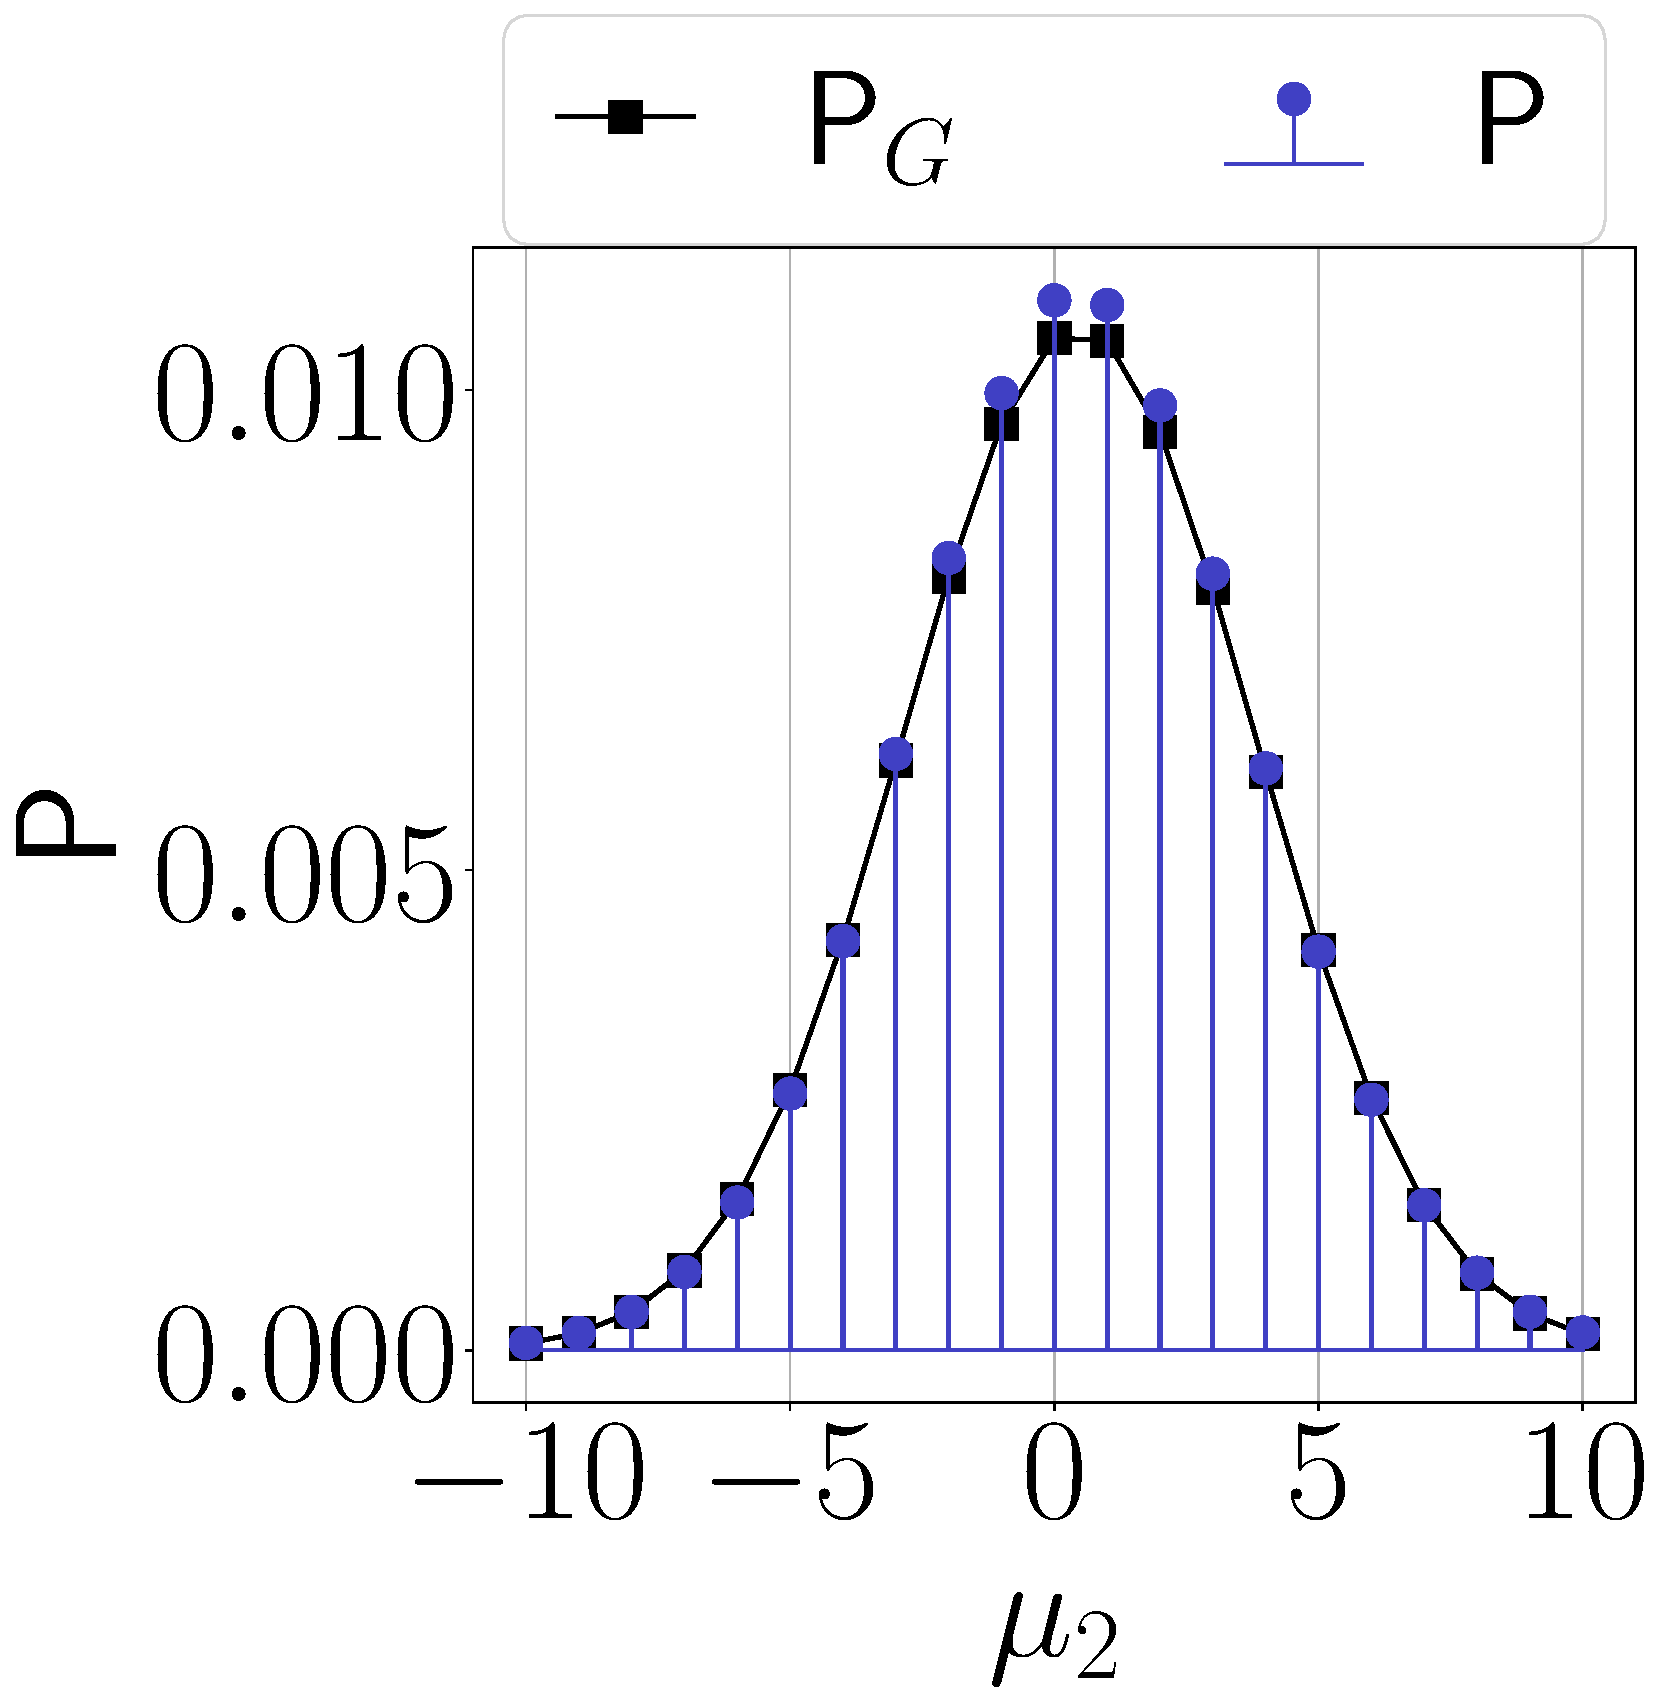
\includegraphics[width=\linewidth]{pics/double-homodyne/dm2.pdf}
\subcaption[]{}
\end{minipage}
    \caption{(a) -- 
     Numerically calculated exact statistical distribution of photon count difference in asymmetrical double homodyne scheme, given by  Eq.~\eqref{eq:accurate-dh}, and calculated distance between this distribution and approximate distribution, given by Eq.~\eqref{eq:Pgood-dh}; (b), (c) -- Projections of exact (blue) and approximate (black) statistical distributions of photon count difference, all calculated for parameters $\alpha=0.25+0.25i$, $\alpha_L=5$, $\eta_1=\eta_3=1$ and $\eta_2=\eta_4=0.75$.
    }\label{fig:dh-statistics}
\end{figure}
%\section{Experiment}\label{sec-experiment}

%%%%%%%%%%%%%%%%%%%%%%%%%%%%
\section{Double homodyne detection}
\label{sec:double-homodyne}
%%%%%%%%%%%%%%%%%%%%%%%%%%%%%%

In the section,
we consider the eight-port double homodyne scheme
depicted in Fig.~\ref{fig:double-homodyne}
(see, e.g., Refs.~\cite{Vogel:bk:2006,lahti2010realistic}).
This measurement scheme is known to allow reconstructing the
Husimi $Q$ function of the signal state~\cite{Richter:98} providing complete information about the signal
state that may be used in CV-QKD protocols. It should be noted that restoration of the
complex amplitude of the state completely serves as the basis for composable security
proofs~\cite{PhysRevLett.93.170504,PhysRevLett.118.200501}.
%~\cite{pirandola2024improvedcomposablekeyrates,pascualgarcía2024improvedfinitesizekeyrates}.


Figure~\ref{fig:double-homodyne} shows two homodyne setups
with elements such as beam splitters BS$_i$
and photodetectors $D_{1,2}^{(i)}$ labeled by the index $i\in\{1,2\}$.
Referring to Fig.~\ref{fig:double-homodyne},
the LO and signal modes are transmitted through
the beam splitters BS$_L$ and BS$_S$, respectively.
Similar to the analysis performed in the previous section,
we assume that the modes are in the coherent states,
$\ket{\alpha}$ and $\ket{\alpha_L}$. So, we
have the amplitudes 
\begin{align}
  &
    \label{eq:amplitudes-SL-i}
    \alpha^{(1)}=C_S\alpha,\quad \alpha^{(2)}=S_S\alpha,
    \notag
  \\
  &
    \alpha_L^{(1)}=C_L\alpha_L,\quad \alpha_L^{(2)}=-iS_L\alpha_L,
\end{align}
where $\alpha^{(i)}$ ($\alpha_{L}^{(i)}$) stands for the amplitude
describing the input coherent state of the signal (LO) mode
of the homodyne labeled by the upper index $i\in \{1,2\}$. 
Note that the phase factor $-i=e^{-i\pi/2}$ in the expression for
$\alpha^{(2)}_L$ is introduced by
a suitably chosen phase shifter placed before
the corresponding input port
of the beam splitter BS$_2$.

It is rather straightforward to see that
the joint statistics of the difference photocount events
is determined by the product
of the Skellam distributions given by
\begin{align}
  &
    \label{eq:P_mu1m2}
    \prob(\mu_1,\mu_2)=\prob_1(\mu_1)\prob_2(\mu_2),
    \quad \mu_i=m_1^{(i)}-m_2^{(i)},
  \\
  &
  \label{eq:Skel-i}
  \prob_i(\mu_i)=e^{-\eta_1^{(i)}|\alpha_1^{(i)}|^2}e^{-\eta_2^{(i)}|\alpha_2^{(i)}|^2}
    \Biggl(\frac{\eta_1^{(i)}|\alpha_1^{(i)}|^2}{\eta_2^{(i)}|\alpha_2^{(i)}|^2}\Biggr)^{\mu_i/2}
    \notag
  \\
  &
    \times
I_{\mu_i}\bigl(2\sqrt{\eta_1^{(i)}\eta_2^{(i)}|\alpha_1^{(i)}|^2|\alpha_2^{(i)}|^2}\bigr),
\end{align}
where, similar to the homodyne scheme,
the amplitudes of the coherent states at the output ports of the beam splitter
BS$_i$
\begin{align}
  &
    \label{eq:amplitudes-i}
    \alpha_1^{(i)}=C_i\alpha^{(i)}+S_i\alpha_L^{(i)},\quad
    \alpha_2^{(i)}=-S_i\alpha^{(i)}+C_i\alpha_L^{(i)}
\end{align}
are expressed in terms of the transmission and reflection amplitudes,
$C_i=\cos\theta_i$ and $S_i=\sin\theta_i$.

We can now apply Eqs.~\eqref{eq:Gaussian}--\eqref{eq:mu_G}
to approximate each Skellam distribution on
the right hand side of Eq.~\eqref{eq:P_mu1m2}
and derive the Gaussian approximation
for the double homodyne scheme in the form:
\begin{align}
  &
  \label{eq:Gaussian-8p}
    \prob_G(\mu_1,\mu_2)=G(\mu_1-\mu_G^{(1)};\sigma_G^{(1)})G(\mu_2-\mu_G^{(2)};\sigma_G^{(2)}),
    \\
  &
    \label{eq:sigma_G-i}
    \sigma_G^{(i)}=
    (\eta_1^{(i)}S_i^2+\eta_2^{(i)}C_i^2) |\alpha_L^{(i)}|^2,
  \\
  &
    \label{eq:mu_G-i}
    \mu_G^{(i)}=
    (\eta_1^{(i)}S_i^2-\eta_2^{(i)}C_i^2) |\alpha_L^{(i)}|^2
    +C_iS_i (\eta_1^{(i)}+\eta_2^{(i)})|\alpha_L^{(i)}| 
    \notag
  \\
  &
    \times
    2\Re\alpha^{(i)} e^{-i\phi},\quad \phi=\arg\alpha_L.
\end{align}
Similar to Eq.~\eqref{eq:Pgood-w-def},
it is useful to put
the probability~\eqref{eq:Gaussian-8p}
into the folowing quadrature form:
\begin{align}
  \label{eq:P_G-x1x2}
  &
    \prob_G(x_1,x_2)=\frac{1}{2\pi\sqrt{\sigma_G^{(1)}\sigma_G^{(2)}}}
    \exp\Bigl\{
    -\frac{(x_1-\Re\alpha e^{-i\phi})^2}{\sigma_1}
    \notag
  \\
  &
    -\frac{(x_2-\Im\alpha e^{-i\phi})^2}{\sigma_2}
    \Bigr\}
\end{align}
where $x_i$ are the quadrature variables given by
\begin{align}
  &
  \label{eq:x-1}
  x_1=
  \frac{1}{2(\eta_1^{(1)}+\eta_2^{(1)})C_1S_1C_S}
  \notag
  \\
  &
    \times
  \Bigl\{
  \frac{\mu_1}{|\alpha_L^{(1)}|}-(\eta_1^{(1)}S_1^2-\eta_2^{(1)}C_1^2) |\alpha_L^{(1)}|
    \Bigr\},
  \\
  &
  \label{eq:x-2}
  x_2=
  \frac{1}{2(\eta_1^{(2)}+\eta_2^{(2)})C_2S_2S_S}
  \notag
  \\
  &
    \times
  \Bigl\{
  \frac{\mu_2}{|\alpha_L^{(2)}|}-(\eta_1^{(2)}S_2^2-\eta_2^{(2)}C_2^2) |\alpha_L^{(2)}|
    \Bigr\},
\end{align}
and relations
\begin{align}
  &
  \label{eq:sigm-i}
    \sigma_1=\frac{\sigma_x^{(1)}}{ 2 C_S^2},
    \quad
    \sigma_2=\frac{\sigma_x^{(2)}}{ 2 S_S^2},
  \\
  &
    \label{eq:sigm-x-i}
    \sigma_x^{(i)}=\frac{\eta_1^{(i)}S_i^2+\eta_2^{(i)}C_i^2}{
    \left[(\eta_1^{(i)}+\eta_2^{(i)})C_iS_i\right]^2
    }
\end{align}
give the quadrature variances $\sigma_1$ and $\sigma_2$.

\begin{figure*}
    \centering
    \begin{subfigure}[c]{.3\linewidth}
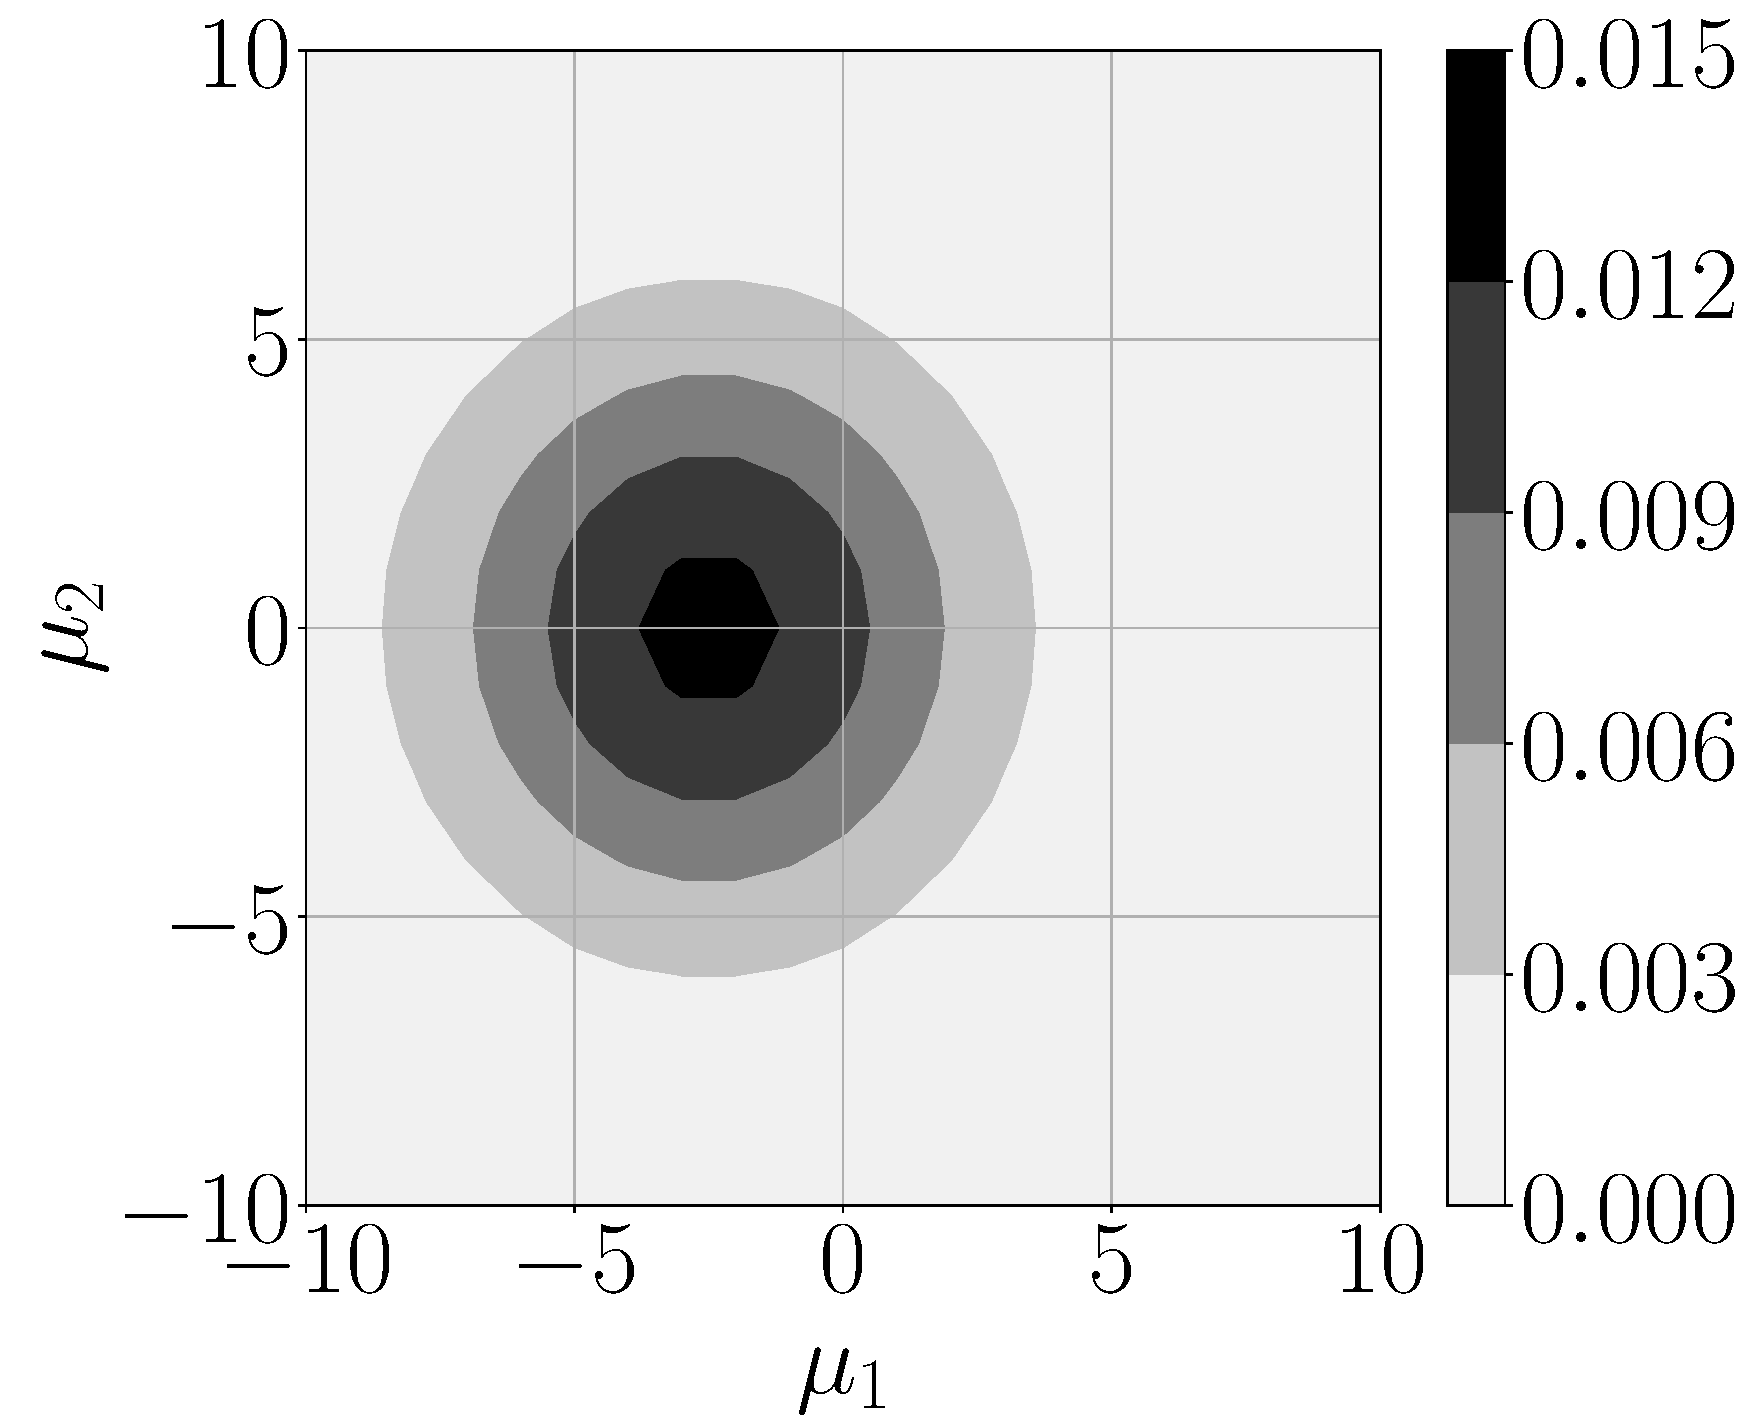
\includegraphics[width=\linewidth]{pics/double-homodyne/1111.pdf}
\caption[]{$\eta_1^{(i)}=1,\eta_2^{(i)}=1$}
        \end{subfigure}
\hfill
        \begin{subfigure}[c]{.3\linewidth}
 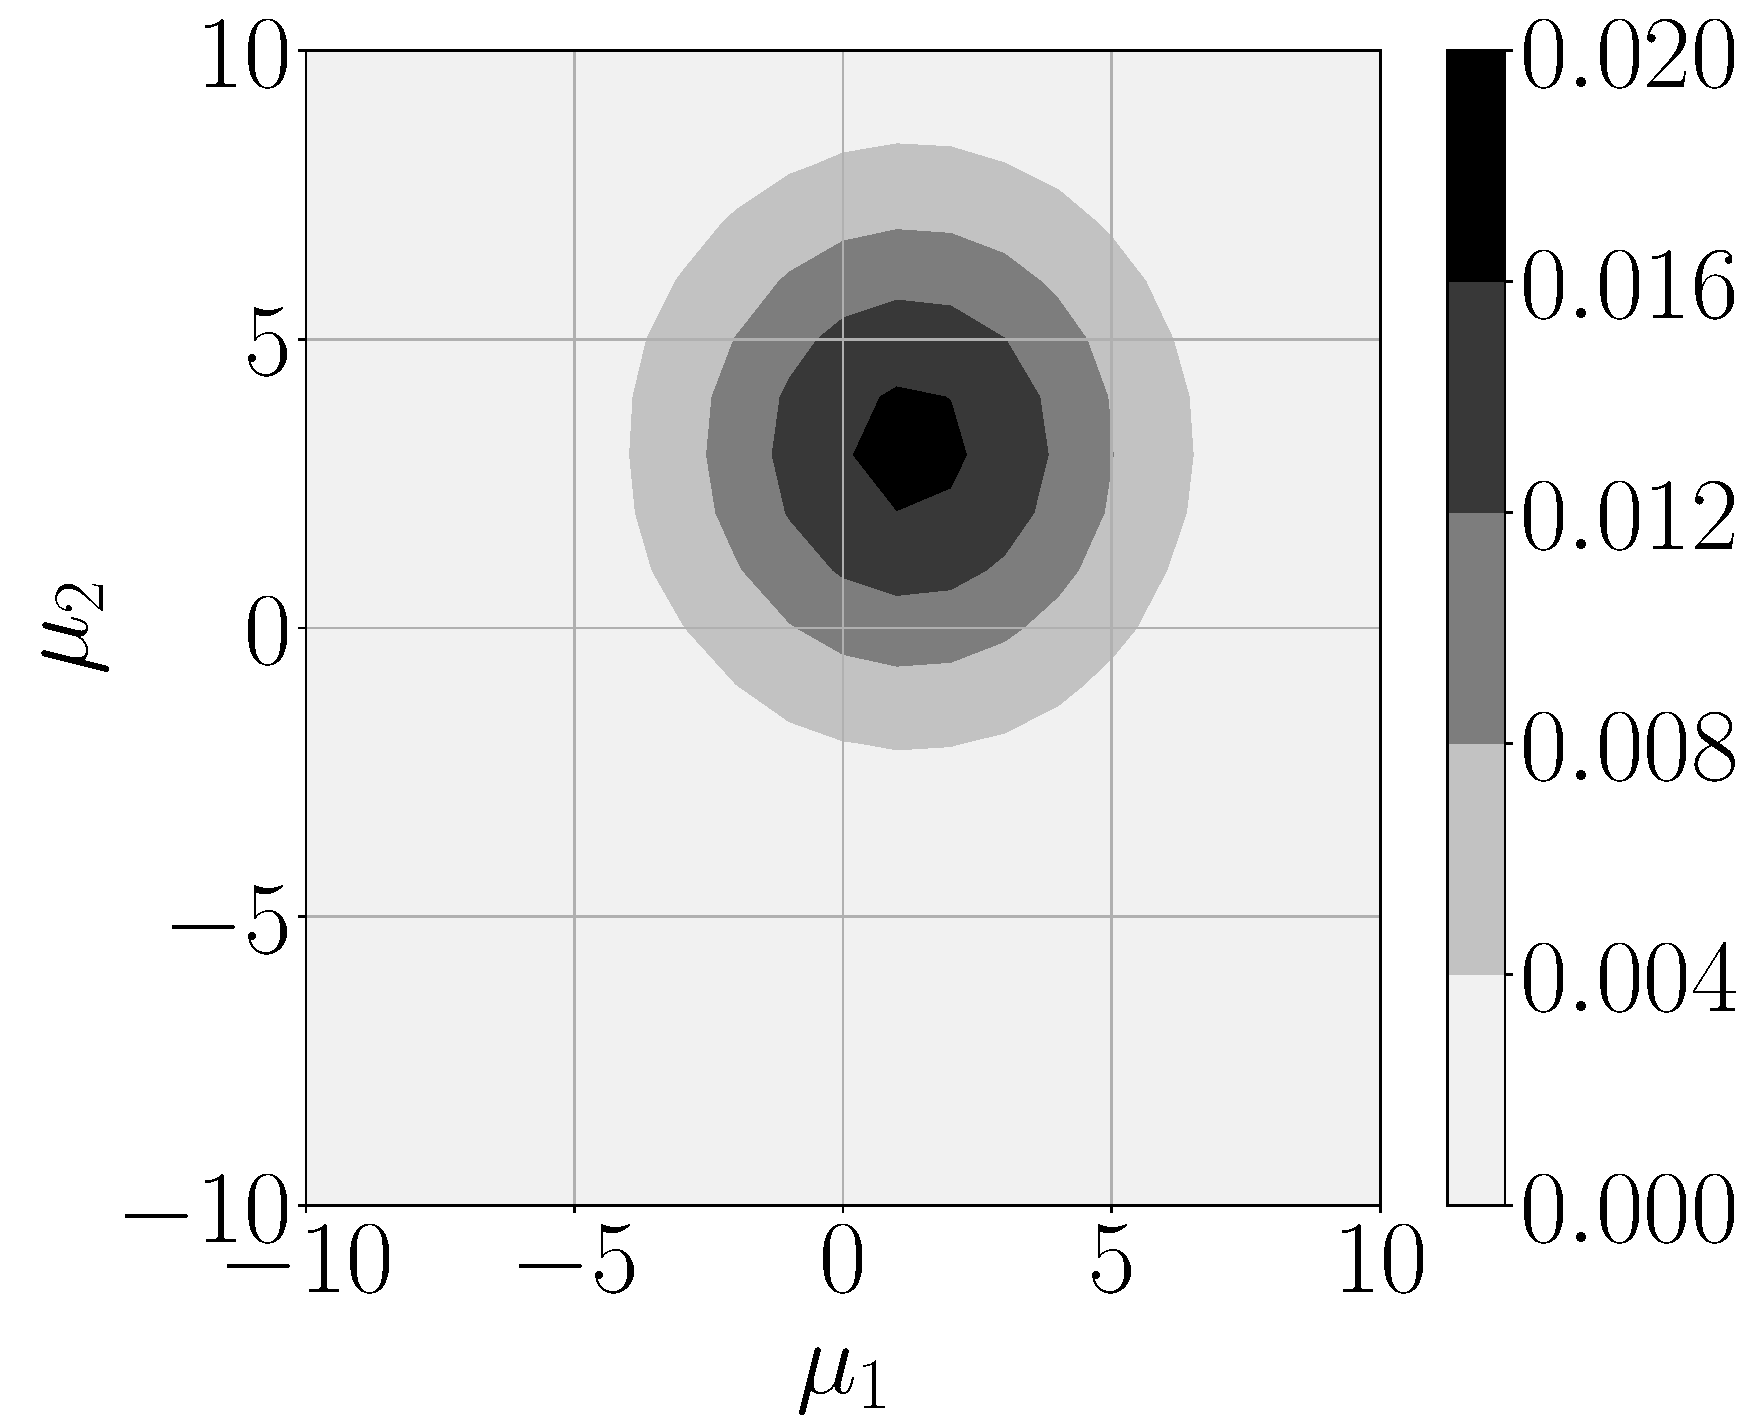
\includegraphics[width=\linewidth]{pics/double-homodyne/10.510.5.pdf}
\caption[]{$\eta_1^{(i)}=1,\eta_2^{(i)}=0.5$}
\end{subfigure}
\hfill
    \begin{subfigure}[c]{.3\linewidth}
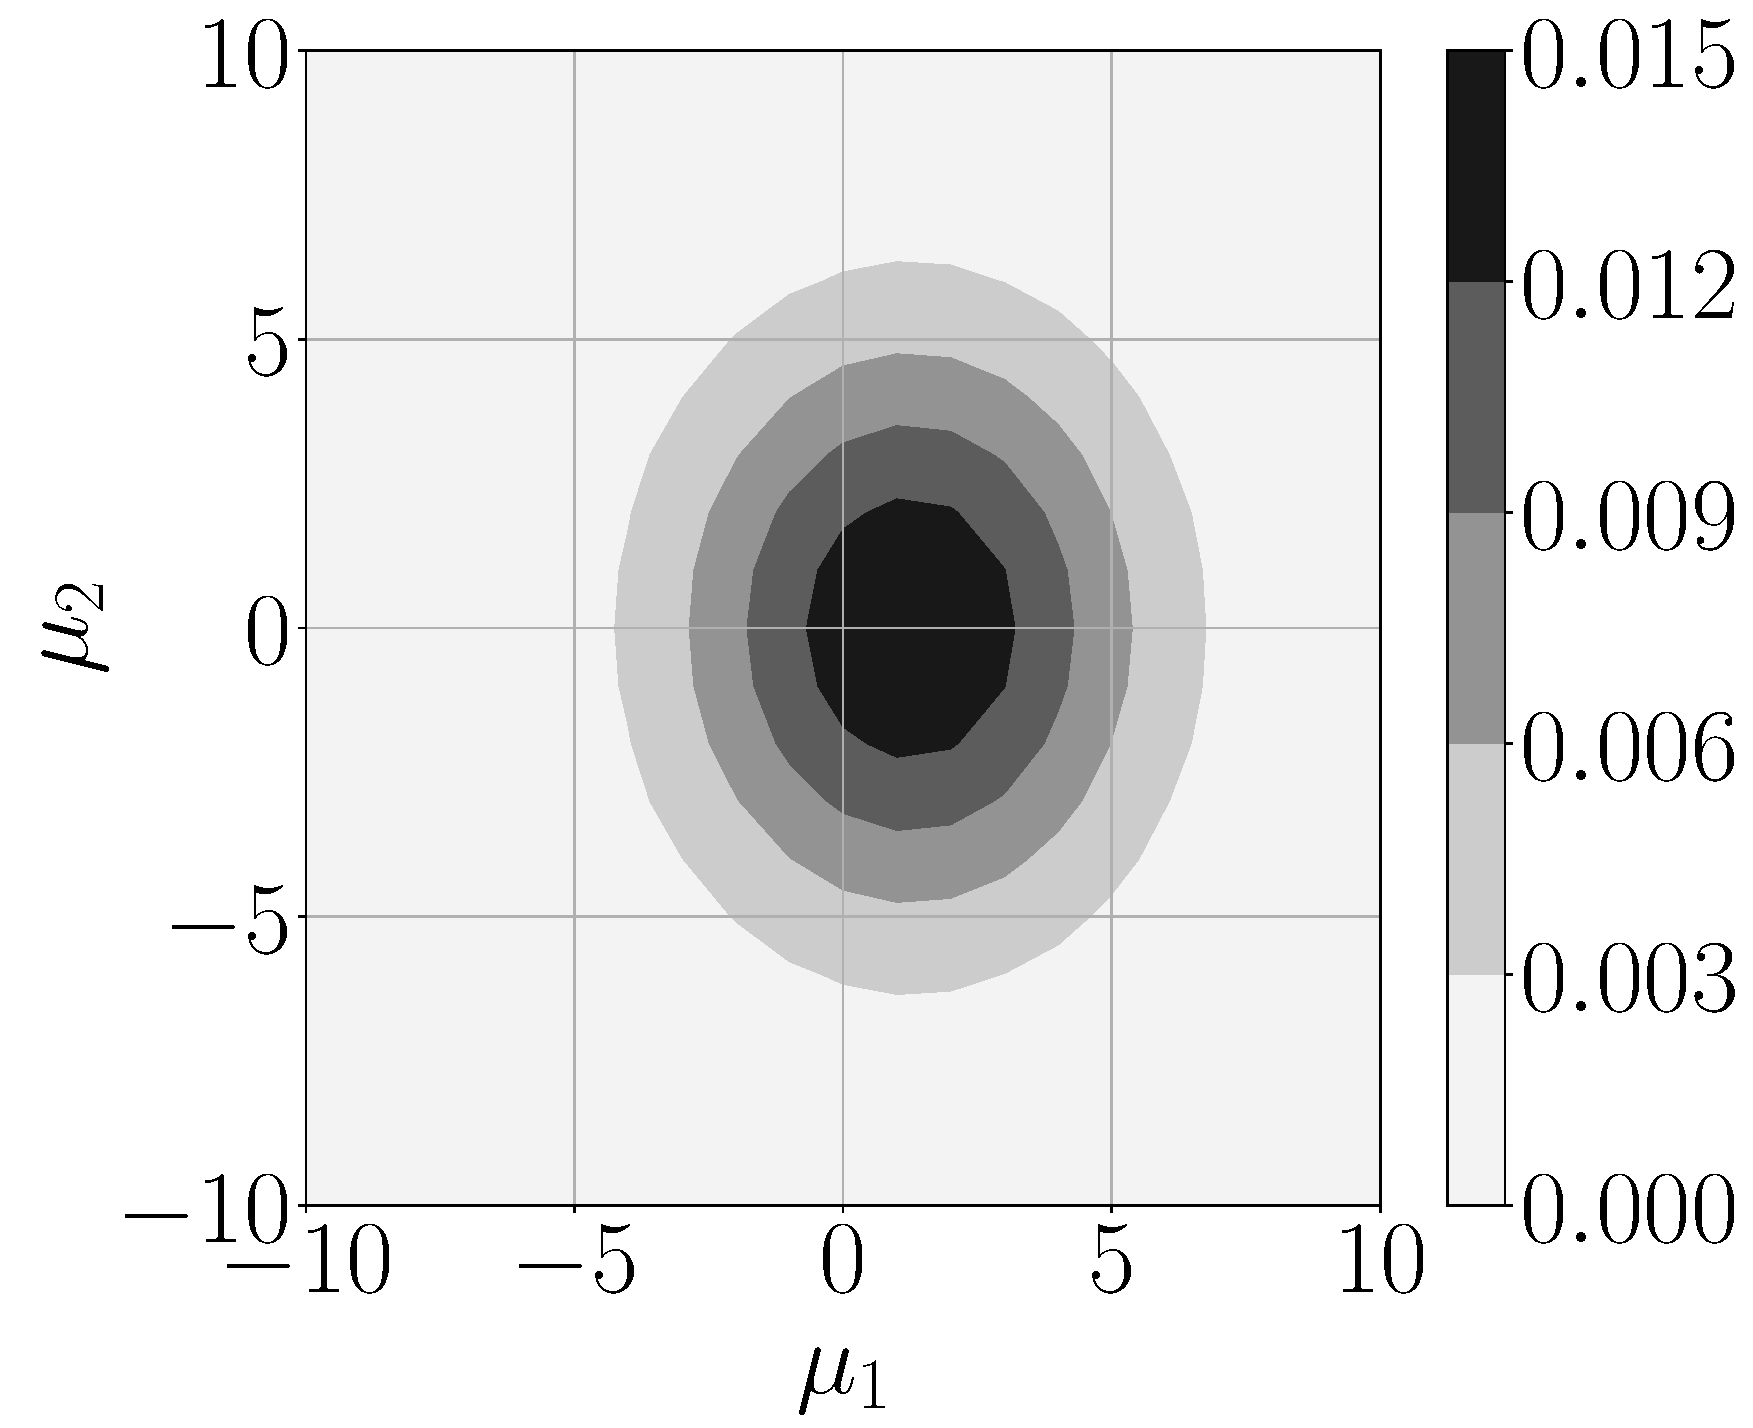
\includegraphics[width=\linewidth]{pics/double-homodyne/1110.5.pdf}
\caption[]{$\eta_1^{(i)}=1,\eta_2^{(1)}=1,\eta_2^{(2)}=0.5$}
        \end{subfigure}
        \caption{Double homodyne statistical distribution of photocount differences
          computed from Eq.~\eqref{eq:P_mu1m2}
          for various detector efficiencies at $\alpha=0.5$ and $\alpha_L=5$.
          All the beam splitters are taken to be balanced.
}
\label{fig:dh-statistics}
\end{figure*}


As in Sec.~\ref{subsec:gauss-hom},
formula~\eqref{eq:P_G-x1x2}
giving the $Q$-symbol of POVM (see Eq.~\eqref{eq:PG-as-avr})
provides the starting point for reconstruction of the POVM
describing the double homodyne measurements.
In the ideal case, where all the beam splitters are balanced
and the photodetection is perfect,
we have
\begin{align}
  &
  \label{eq:P0-hetero}
    \prob_{G}^{(0)}(x_1,x_2)=\frac{|\avr{z|\alpha}|^2}{\pi |\alpha_L|^2},\quad
|\avr{z|\alpha}|^2=e^{-|z-\alpha|^2},
\end{align}
where
\begin{align}
  \label{eq:z}
    z=(x_1+ix_2) e^{i\phi},\quad     x_i=\frac{\mu_i}{|\alpha_L|}.
\end{align}
So, the POVM is proportional to a projector onto the coherent state
$\ket{z}\equiv\ket{(x_1+ix_2)e^{i\phi}}$:
\begin{align}
  \label{eq:POVM-hetero-ideal}
    \hat{\Pi}_G^{(0)}(x_1,x_2)=\frac{1}{\pi |\alpha_L|^2} \ket{z}\bra{z}.
\end{align}
For non-ideal measurements, the probability~\eqref{eq:P_G-x1x2}
can be expressed
as a Gaussian superposition of the coherent state Husimi functions
with the help of the convolution relation~\eqref{eq:convolution}
as follows
\begin{align}
  \label{eq:P_G-x1x2-2}
  &
    \prob_G(x_1,x_2)=\frac{\sqrt{\sigma_1\sigma_2}}{2\pi\sqrt{\sigma_G^{(1)}\sigma_G^{(2)}}}
\int \dd \beta_1\dd \beta_2
    G(x_1-\beta_1;\sigma_N^{(1)})
    \notag
  \\
  &
    \times
    G(x_2-\beta_2;\sigma_N^{(2)})
    |\avr{\beta e^{i\phi}|\alpha}|^2,\quad \beta=\beta_1+i\beta_2,
\end{align}
where the excess noise variance
$\sigma_N^{(i)}$ is determined by the relation
\begin{align}
  &
    \label{eq:sigm-N-i}
    2\sigma_{N}^{(i)}=\sigma_i-1.
\end{align}
The corresponding expression for the POVM reads
\begin{align}
  &
  \label{eq:povm-hetero}
    \hat{\Pi}_G(x_1,x_2)=\frac{\sqrt{\sigma_1\sigma_2}}{2\pi\sqrt{\sigma_G^{(1)}\sigma_G^{(2)}}}
\int \dd \beta_1\dd \beta_2
    G(x_1-\beta_1;\sigma_N^{(1)})
    \notag
  \\
  &
    \times
    G(x_2-\beta_2;\sigma_N^{(2)})
    \ket{\beta e^{i\phi}}\bra{\beta e^{i\phi}}.
\end{align}

An important point is that
the results given by Eq.~\eqref{eq:P_G-x1x2-2}
and Eq.~\eqref{eq:povm-hetero}
are well defined only if $\sigma_1$ and $\sigma_2$
are both above unity,
so that the excess noise variances~\eqref{eq:sigm-N-i} are
positive.
From Eq.~\eqref{eq:sigm-i},
this requires that conditions
$\sigma_x^{(1)}\ge 2 C_S^2$
and $\sigma_x^{(2)}\ge 2 S_S^2$ be met.

When the beam splitter BS$_S$
is balanced $2 C_S^2=2 S_S^2=1$
and inequality (see Eq.~\eqref{eq:sigma-x-min})
\begin{align}
  \label{eq:sigma-x-min-i}
  \sigma_x^{(i)}\ge \Biggl(
\frac{\sqrt{\eta_1^{(i)}}+\sqrt{\eta_2^{(i)}}}{\eta_1^{(i)}+\eta_2^{(i)}}
  \Biggr)^2\ge 1
\end{align}
ensures applicability of the expression for the POVM.
Otherwise, either $2 C_S^2$ or $2 S_S^2$ will be above unity,
and our results are valid only if
the value of the corresponding variance $\sigma_x^{(i)}$ is sufficiently high.
For example, at $\eta_{1,2}^{(i)}=\eta<1/2$,
the minimal values of $\sigma_x^{(i)}$ are higher than $2$
(see Eq.~\eqref{eq:sigma-x-min-i})
and the noise variance will be positive at
any disbalance of the signal mode beam splitter
because $\max\{2 C_S^2,2 S_S^2\}\le 2$.
When the noise variance is negative,
the POVM reconstruction procedure
needs to be generalized.
We shall present details on this generalization
in the next section.
Meanwhile,
in the remaining part of this section,
we confine ourselves to the cases where $\sigma_N^{(i)}$ are positive.

The effects of photodetection asymmetry
are illustrated in Fig.~\ref{fig:dh-statistics}
which presents numerical results for
the double homodyne distribution~\eqref{eq:P_mu1m2}
in the photocont difference $\mu_1$-$\mu_2$ plane.
Referring to Fig.~\ref{fig:dh-statistics},
in addition to the shift of the distribution,
the asymmetry induced difference of the variances
at $\eta_1^{(1)}+\eta_2^{(1)}\ne \eta_1^{(2)}+\eta_1^{(2)}$
manifests itself as the two dimensional anisotropy
of the double homodyne distribution.

%%%%%%%%%%%%%%%%%%%%%%%%%%%%
\section{Positive operator-valued measure and squeezed states}
\label{sec:gen-POVM}
%%%%%%%%%%%%%%%%%%%%%%%%%%%%%%

From Eq.~\eqref{eq:sigm-N-i},
the expression for the POVM
in the form of incoherent gaussian superposition
of coherent states is justified only if
both the quadrature variances, $\sigma_1$ and $\sigma_2$,
exceed unity.
In this section, we show that our procedure employed
for derivation of the double homodyne POVM can be
suitably generalized by enlarging a set of the pure states to include
the squeezed coherent states
\begin{align}
  \label{eq:squeezed-def}
  \ket{\beta,\xi}=\hat{D}(\beta)\hat{S}(\xi)\ket{0},
\end{align}
where $\hat{D}(\beta)$ ($\hat{S}(\xi)$) is the displacement
(squeezing) operator  given by
\begin{align}
\label{eq:D-S-def}
\hat{D}(\beta) =
e^{\beta\hcnj{\hat{a}}-\beta^*\hat{a}}, \quad
    \hat{S}(\xi)=e^{\frac{1}{2}\left(\xi\hat{a}^{\dag2}-\xi^*\hat{a}^2\right)},
\end{align}
$\beta$ and $\xi$ are the complex-valued amplitude
and the squeeze parameter, respectively. 

To this end, we consider the case, where
the squeeze parameter is given by
\begin{align}
  \label{eq:sq-param}
  \xi=r e^{2 i \phi},\quad
  r\in\mathbb{R}
\end{align}
and the non-normalized Husimi distribution
for the squeezed state~\eqref{eq:squeezed-def} takes
the form
(see, e.g., the textbook~\cite{Gerry:bk:2005})
\begin{align}
\label{eq:squeezed-Q}
  &
    |\langle\beta,r e^{2 i \phi}|\alpha\rangle|^2=\frac{1}{\cosh r}
    \exp\Bigl\{-
    \frac{e^{-r}}{\cosh r}{}
    \left(\tilde{\beta}_1e^{r}-\tilde{\alpha}_1\right)^2
    \notag
  \\
    &-\frac{e^{r}}{\cosh r}{}\left(\tilde{\beta}_2e^{{-r}}-\tilde{\alpha}_2\right)^2
      \Bigr\},
  \\
  &
    \label{eq:tbeta-alpha}
    \tilde{\beta}=\tilde{\beta}_1+ i \tilde{\beta}_2=\beta e^{-i\phi},
    \quad
    \tilde{\alpha}=\tilde{\alpha}_1+ i \tilde{\alpha}_2=\alpha e^{-i\phi}.
\end{align}
By using
this squeezed state distribution instead
of the coherent state one 
given in Eq.~\eqref{eq:POVM-hetero-ideal},
we are led to the expressions for
the noise variances modified as follows
\begin{align}
  \label{eq:sigma_N-sq-1}
  &
    2\sigma_N^{(1,2)}=\sigma_{1,2}-e^{\pm r}\cosh r.
\end{align}
These expressions present the
extension of the relations~\eqref{eq:sigm-N-i}
to the case with non-vanishing squeeze parameter.
As an immediate consequence of Eq.~\eqref{eq:sigma_N-sq-1},
we find that
the conditions for the noise variances to be positive definite
can be written in the form of two inequalities 
\begin{align}
  \label{eq:sigma_N-sq-2}
  &
    4\sigma_N^{(1)}=\delta_1-e^{2r}\ge 0,
    \quad
    4\sigma_N^{(2)}=\delta_2-e^{-2r}\ge 0,
\end{align}
where the quadrature variance parameters
\begin{subequations}
  \label{eq:delta_12}
\begin{align}
  \label{eq:delta_1}
  &
    \delta_1=2\sigma_1-1=(q+1)\sigma_x^{(1)}-1\ge q=\frac{S_S^2}{C_S^2},
  \\
  &
    \label{eq:delta_2}
    \delta_2=2\sigma_2-1=(q^{-1}+1)\sigma_x^{(2)}-1\ge q^{-1}=\frac{C_S^2}{S_S^2}
\end{align}
\end{subequations}
are expressed in terms of
the disbalance
(reflection-to-transmission)
ratio of the input beam splitter, $q$,
and the parameters $\sigma_{x}^{(1)}$
and $\sigma_{x}^{(2)}$
(see Eq.~\eqref{eq:sigm-x-i})
that cannot be smaller than unity
(see Eq.~\eqref{eq:sigma-x-min-i}): $\sigma_x^{(i)}\ge 1$.

In our subsequent analysis,
we assume without the loss of generality
that the reflectance of the input beam splitter BS$_S$ is
larger than its transmittance,
so that the disbalance ratio is above unity 
\begin{align}
  \label{eq:q-param}
  &
    q=\frac{1-C_S^2}{C_S^2}=\frac{S_S^2}{C_S^2}\ge 1.
\end{align}
As is shown in Fig.~\ref{fig:squeezing},
this implies that the variance $\delta_1$
is above unity: $\delta_1\ge q\ge 1$,
whereas the minimal value of $\delta_2$
is $q^{-1}\le 1$.
It is illustrated that
the noise variances are positive
provided the squeeze parameter $r$
is ranged between
the endpoints of the interval given by
\begin{align}
  \label{eq:r1-r2}
  &
    r\in[r_2,r_1],\;
    r_1=\ln\delta_1^{1/2},
    \;
    r_2=\max\{\ln\delta_2^{-1/2},0\}.
\end{align}

\begin{figure}
    \centering
    \includegraphics[width=0.9\linewidth, page={2}]{tikz_article.pdf}
    \caption{An illustration for the conditions for the noise variances, see Eqs.~\eqref{eq:sigma_N-sq-2}-\eqref{eq:r1-r2}.
    Solid grey lines represent the exponents $e^{\pm2r}$. Dashdotted black, red and blue lines are the independent on $r$ functions $q$ and $q^{-1}$, $\delta_1$ and $\delta_2$ respectively. Solid purple line is the interval of squeezing parameter $r\in[r_2,r_1]$, solid red (blue) line %with pointing arrow of the same color 
    is the magnitude of $4\sigma_N^{(1)}$ ($4\sigma_N^{(2)}$) at $r$.}
    \label{fig:squeezing}
\end{figure}

An important point is that
the value of the squeeze parameter
is not uniquely determined
by the conditions~\eqref{eq:sigma_N-sq-2}.
We have a unique value of
the squeeze parameter only in  the limiting case
of perfect homodyne measurements
with $\sigma_{x}^{(1)}=\sigma_{x}^{(2)}=1$
and $\delta_{1}=\delta_{2}^{-1}=q$.
In this case, the squeeze parameter is
unambiguously defined
\begin{align}
  &
  \label{eq:r-ideal}
  r_1=r_2=\rho=\frac{1}{2}\ln q=\ln\sqrt{\frac{1-C_S^2}{C_S^2}}
\end{align}
and the probability~\eqref{eq:P_G-x1x2}
expressed in terms of the distribution~\eqref{eq:squeezed-Q}
\begin{align}
  &
    \label{eq:P_G-ideal}
  \prob_{G}^{(1)}(x_1,x_2)=\frac{\cosh \rho}{2\pi |\alpha_L^{(1)}\alpha_L^{(2)}|}
    |\avr{\beta e^{i\phi},\rho e^{2i\phi}|\alpha}|^2,
  \\
  &
    \label{eq:beta-ideal}
    \beta=e^{-\rho}x_1+i e^{\rho} x_2
\end{align}
yields the POVM
\begin{align}
    \label{eq:Pi_G-ideal}
    \hat{\Pi}_{G}^{(1)}(x_1,x_2)&=\frac{\cosh \rho}{2\pi |\alpha_L^{(1)}\alpha_L^{(2)}|}
    \notag
  \\
  &
  \times
    \ket{\beta e^{i\phi},\rho e^{2i\phi}}\bra{\beta e^{i\phi},\rho e^{2i\phi}},
\end{align}
which is propotional to the pure squeezed state
$\ket{\beta e^{i\phi},\rho e^{2i\phi}}$.
The result~\eqref{eq:r-ideal}
was reported in Ref.~\cite{genoni2014general}.

When the homodyne measurements are not
perfect due to unbalanced beam splitters and nonideal photodetectors,
the squeeze parameter is no longer uniquely defined.
So, in the interval~\eqref{eq:r1-r2},
we have the decomposition of
the probability~\eqref{eq:P_G-x1x2}
\begin{align}
  \label{eq:P_G-gen-x1x2-2}
  &
    \prob_G(x_1,x_2)=\frac{\sqrt{\sigma_1\sigma_2}}{2\pi\sqrt{\sigma_G^{(1)}\sigma_G^{(2)}}}
\notag
  \\
  &
    \times
    \int \dd \beta_1\dd \beta_2
    G(x_1e^{-r}-\beta_1;\sigma_N^{(1)}(r)e^{-2r})
    \notag
  \\
  &
    \times
    G(x_2e^{r}-\beta_2;\sigma_N^{(2)}(r)e^{2r})
    |\avr{\beta e^{i\phi},r e^{2i\phi}|\alpha}|^2 
\end{align}
that varies with the squeeze parameter $r$.
Similarly,
the corresponding POVM 
\begin{align}
  \label{eq:Pi_G-gen-x1x2}
  &
    \hat{\Pi}_G(x_1,x_2)=\frac{\sqrt{\sigma_1\sigma_2}}{2\pi\sqrt{\sigma_G^{(1)}\sigma_G^{(2)}}}
\notag
  \\
  &
    \times
    \int \dd \beta_1\dd \beta_2
    G(x_1e^{-r}-\beta_1;\sigma_N^{(1)}(r)e^{-2r})
    \notag
  \\
  &
    \times
    G(x_2e^{r}-\beta_2;\sigma_N^{(2)}(r)e^{2r})
    \notag
  \\
  &
    \times
    \ket{\beta e^{i\phi},r e^{2i\phi}}\bra{\beta e^{i\phi},r e^{2i\phi}}
\end{align}
decomposed into
the Gaussian incoherent superposition
of the pure squeezed states explicitly depends on the value of $r$.
Our analysis suggests that  the ambiguity (non-uniqueness) of
the Gaussian represention~\eqref{eq:Pi_G-gen-x1x2} for the double-homodyne
POVM is a universal feature coming into play
in the presence of imperfections.
Even when $\delta_2\ge 1$ and
the coherent-state represention~\eqref{eq:povm-hetero} for the POVM is well-defined,
the photocount statistics can be reproduced using
the squeezed-state representation~\eqref{eq:Pi_G-gen-x1x2}
with $0<r \le r_1$.
One of the way to make the Gaussian POVM decomposition unique
is to place additiona constraints
on the noise variances that would fix the value of the squeeze parameter.
For example,
the squeeze parameter would take the minimal (maximal) value:
$r=\min\{r_1,r_2\}$ ($r=\max\{r_1,r_2\}$)
provided the constraint requires minimization of
the noise variance $\sigma_N^{(2)}$ ($\sigma_N^{(1)}$).
%%%%%%%%%%%%%%%%%%%%%%%%%%%%%
\section{Incorporating measurement imperfections into the GG02 CV-QKD Protocol}
\label{sec:protocol}

In this section, we apply our results on asymmetric measurements to analyze the Gausssian modulated coherent state (GMCS, or GG02~\cite{PhysRevLett.88.057902}) CV-QKD protocol. Specifically, we compute the mutual information, Holevo information, and asymptotic secret key fraction under an untrusted noise scenario, in order to assess the impact of measurement asymmetry on the protocol’s security.

In the GG02 protocol, Alice prepares an ensemble of coherent states whose amplitudes $\alpha$ are drawn from a zero-mean Gaussian distribution, denoted by $G(0; \tilde V_{\ind{mod}})$, where $\tilde V_{\ind{mod}}$ is the modulation variance. The probability distributions of the quadrature operators $\hat{q}$ and $\hat{p}$ are then given by
\begin{align}
\label{eq:p(Vmod)}
    p(\hat{q})=p(\hat{p})\equiv p(\hat{q}|\hat{p})=G(0;  V_{\ind{mod}}=4\tilde V_\ind{mod})
\end{align}
where we used the relation $2\hat{a}=\hat{q}+i\hat{p}$, which implies $4V(\alpha)\equiv 4\tilde V_{\ind{mod}}=V(\hat{q})=V(\hat{p})\equiv V_{\ind{mod}}$. After transmission through a Gaussian channel, which attenuates the coherent amplitude by a factor of $\sqrt{T}$, where $T$ is the channel transmission, the state transforms as $\ket{\alpha}\mapsto\ket{\sqrt{T}\alpha}\equiv\ket{\tilde\alpha}$. The quadratures are then measured by Bob. The resulting quadrature distribution is:
\begin{align}
\label{eq:pB}
    &p_{\ind{B}}=\int\mathop{\dd q\dd p }p(\hat{q},\hat{p})\Tr\ket{\tilde \alpha}\bra{\tilde \alpha}\hat{\Pi}=\frac{1}{T}\int\mathop{\dd \tilde\alpha }p(\tilde\alpha)\bra{\tilde\alpha}\hat{\Pi}\ket{\tilde\alpha}\notag\\&=\frac{1}{T}\int\mathop{\dd\tilde\alpha}p(\tilde\alpha)Q_{\Pi}(\tilde\alpha),
\end{align}
where $\hat{\Pi}$ is the POVM describing the measurements, and $Q_{\Pi}(\alpha)$ is its' corresponding $Q$-function. Note that the variance $p(\tilde \alpha)$ is $TV_{\ind{mod}}$.

Assuming that Bob performs homodyne detection, the variance of the distribution $p_{\ind{B}}$ in Eq.~\eqref{eq:pB} is given by
\begin{equation}
\label{eq:VB_HOM_nonoise}
    V_{\ind{B}}(\hat q|\hat p)\equiv V_{\ind{B}}^{\ind{HOM}}=%{T} V_{\ind{mod}}+\sigma_N+1=
    {T} V_{\ind{mod}}+\sigma_x.
\end{equation}
Analogously, adding any stochastic noise (e.g., channel excess noise) with variance $\xi$ modifies the total variance $V_{\ind{B}}^{\ind{HOM}}$ as
\begin{align}
\label{eq:VB_hom}
    V_{\ind{B}}^{\ind{HOM}}={T} V_{\ind{mod}}+\sigma_x+\xi.
\end{align}
From this, the signal-to-noise ratio (SNR) and the mutual information between Alice and Bob are given by
\begin{align}
\label{eq:SNR_hom}
    &\ind{SNR}^{\ind{HOM}} =\frac{TV_{\ind{mod}}}{\sigma_x+\xi},\\
    \label{eq:IAB_hom}
    &I_{\ind{AB}}^{\ind{HOM}}=\frac{1}{2}\log\left[1+\ind{SNR}^{\ind{HOM}}\right]\,
\end{align}
where all logarithms are base 2.

Mathematically, the GG02 protocol is equivalent to Alice preparing a two-mode squeezed vacuum state, performing simultaneous measurements of both quadratures on one mode, and sending the other mode through a quantum channel to Bob. The covariance matrix after transmission through a noisy channel is given by~\cite{laudenbach2018continuous}
\begin{align}
\label{eq:sigma_AB}
    &\Sigma_{\ind{AB}}=
    \begin{pmatrix}
        V\mathbb{I}&\sqrt{T(V^2-1)}\sigma_Z\\
        \sqrt{T(V^2-1)}\sigma_Z&(T(V-1)+1+\xi)\mathbb{I}
    \end{pmatrix}\notag\\
    &\equiv\begin{pmatrix}
        a\mathbb{I}&c\sigma_Z\\
        c\sigma_Z&b\mathbb{I}
    \end{pmatrix}
\end{align}
where $V=V_{\ind{mod}}+1$ is the quadrature operator variance in shot-noise units (SNU). 
Here, the shot noise variance is normalized to 
unity and added to the modulation variance due to the uncertainty relation and their mutual 
stochastic independence. The identity matrix is $\mathbb{I}=\ind{diag}(1,1)$, 
and $\sigma_Z=\ind{diag}(1,-1)$.

To calculate the Holevo information, we assume a purification attack. In the untrusted noise scenario, the asymmetric noise is accessible to Eve and modifies the covariance matrix $\Sigma_{\ind{AB}}$ as $b\mapsto b+\sigma_N= V_{\ind{B}}^{\ind{HOM}}$, yielding
\begin{align}
\label{eq:Sigma_AB_hom}
    \Sigma_{\ind{AB}}'=\begin{pmatrix}
        a\mathbb{I}&c\sigma_Z\\
        c\sigma_Z&V_{\ind{B}}^{\ind{HOM}}\mathbb{I}
    \end{pmatrix}.
\end{align}
Eve's entropy, $S_{\ind{E}}=S_{\ind{AB}}$, is calculated from the symplectic eigenvalues of $\Sigma'_{\ind{AB}}$ as~\cite{Weed:rmp:2012}
\begin{align}
\label{eq:nu12}
    &\nu_{1,2} =\frac{1}{2}\left(z\pm\left[V_{\ind{B}}^{\ind{HOM}}-a\right]\right),\notag\\ &z=\sqrt{\left(a+V_{\ind{B}}^{\ind{HOM}}\right)^2-4c^2}.
\end{align}

Bob’s partial measurement of a single quadrature, described by the matrix $\Pi_{q,p}$, where $\Pi_q=\ind{diag}(1,0)$ and $\Pi_p=\ind{diag}(0,1)$ are measurements of $\hat{q}$ and $\hat{p}$ quadratures, respectively, transforms Alice's state covariance matrix as~\cite{laudenbach2018continuous}
\begin{align}
    \label{eq:AB}
    &\Sigma_{\ind{A}|\ind{B}}=a\mathbb{I}-c^2\sigma_Z[\Pi_{q,p}\ b\mathbb{I}\ \Pi_{q,p}]^{-1}\sigma_Z^{\ind T}\notag\\
    &=a\mathbb{I}-\frac{c^2}{b}\Pi_{q,p}.
\end{align}
The corresponding symplectic eigenvalue $\nu_3$ of $\Sigma_{\ind{A}|\ind{B}}$ is
 \begin{align}
     \label{eq:nu3}
     &\nu_3=\sqrt{a\left(a-\frac{c^2}{b}\right)}\notag\\&=\sqrt{V\left(V-\frac{T(V^2-1)}{T(V-1)+1+\xi}\right)},
 \end{align}
which allows us to calculate the conditional entropy $S_{\ind{E}|\ind{B}}=S_{\ind{A}|\ind{B}}$. The Holevo information is then given by
\begin{align}
\label{eq:chi}
    &\chi_{\ind{EB}}\equiv S_{\ind{E}}-S_{\ind{E}|\ind{B}}=S_{\ind{AB}}-S_{\ind{A}|\ind{B}}\notag\\&=\sum_{i=1,2}g(\nu_i)-g(\nu_3),
\end{align}
where
\begin{align}
\label{eq:g(nu)}
    g(\nu)=\frac{\nu+1}{2}\log \frac{\nu+1}{2}-
    \frac{\nu-1}{2}\log\frac{\nu-1}{2},
\end{align}
and the asymptotic secret fraction is given by
\begin{equation}
\label{eq:r}
    R=\beta I_{AB}-\chi_{EB},
\end{equation}
where $\beta$ is the reconciliation efficiency.

Assuming that Bob performs double homodyne detection~\cite{PhysRevLett.93.170504}, analogously to Eq.\eqref{eq:VB_hom}-\eqref{eq:IAB_hom}, we have
\begin{align}
    V_{\ind{B}}^{\ind{DHOM}}&=
    TV_{\ind{mod}}+\frac{\sigma_1+\sigma_2}{2}+\xi
    \\
    \ind{SNR}^{(i)}&=\frac{2TV_{\ind{mod}}}{\sigma_i+2\xi_i},\qquad \xi_1=C_S^2\xi,\quad \xi_2=S_S^2\xi\\
    I_{\ind{AB}}^{\ind{DHOM}}&=\frac{1}{2}\sum_{i=1,2}\log(1+\ind{SNR}^{(i)}).
\end{align}

Note that while the squeezing parameter $r$ affects the decomposition of noise components (see Eq.~\eqref{eq:sigma_N-sq-1}), the protocol ultimately depends only on the observed variances $\sigma_{1,2}$. Thus, the specific form of the double homodyne POVM is irrelevant for the security analysis.

Eve's entropy $S_{\ind{E}}$ is calculated using the symplectic eigenvalues of the covariance matrix
\begin{align}
\label{eq:Sigma_AB_dhom}
    \Sigma_{\ind{AB}}'=\begin{pmatrix}
        a\mathbb{I}&c\sigma_Z\\
        c\sigma_Z&V_{\ind{B}}^{\ind{DHOM}}\mathbb{I}
    \end{pmatrix}.
\end{align}

Double homodyne detection of Bob’s mode transforms Alice’s conditional covariance matrix as
\begin{align}
    \label{eq:AB_dhom}&\Sigma_{\ind{A}|\ind{B}}=
    a\mathbb{I}-c^2\sigma_Z[b\mathbb{I}+\mathbb{I}]^{-1}\sigma_Z^{\ind T}\notag\\&=\left(a-\frac{c^2}{b+1}\right)\mathbb{I},
\end{align}
resulting in symplectic eigenvalue $\nu_3$ in the form
\begin{align}
    \nu_3=a-\frac{c^2}{b+1},
\end{align}
which is then used in Eq.~\eqref{eq:chi} to compute the Holevo information.

The effects of detection asymmetry on mutual information, Holevo information, and the asymptotic secret key rate are illustrated in Fig.~\ref{fig:homodyne-all} for homodyne detection and Fig.~\ref{fig:double-homodyne-all} for double homodyne detection. Our numerical results for the homodyne case are consistent with Ref.~\cite{ruiz2023effects}. The dependence of the asymptotic secret key rate on channel length in the presence of asymmetrical detection is shown in Fig.~\ref{fig:r-of-l-all}. These results indicate that in the untrusted noise scenario, asymmetrical homodyne detection does not offer any advantage, while double homodyne detection consistently yields better performance.

\begin{figure*}
    \centering
    \begin{subfigure}[c]{.3\linewidth}
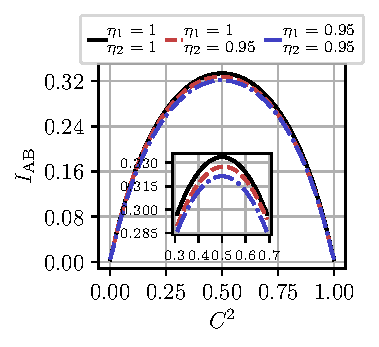
\includegraphics[width=\linewidth, trim={.2cm .3cm .4cm .35cm},clip]{pics/qkd/hom/IAB.pdf}
\caption[]{$I_{\ind{AB}}$}
        \end{subfigure}
\hfill
        \begin{subfigure}[c]{.3\linewidth}
 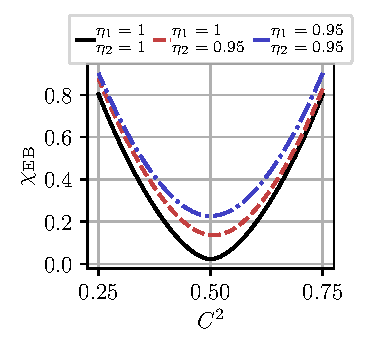
\includegraphics[width=\linewidth, trim={.2cm .3cm .4cm .35cm},clip]{pics/qkd/hom/chi.pdf}
\caption[]{$\chi_{\ind{EB}}$}
\end{subfigure}
\hfill
    \begin{subfigure}[c]{.3\linewidth}
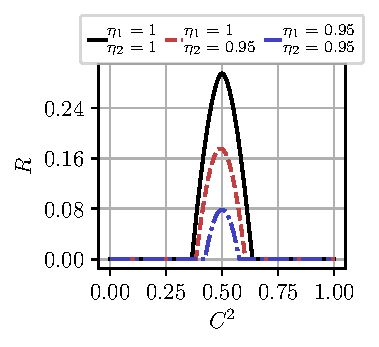
\includegraphics[width=\linewidth, trim={.2cm .3cm .4cm .35cm},clip]{pics/qkd/hom/r.pdf}
\caption[]{$R$}
        \end{subfigure}
        \caption{(a) Mutual information, (b) Holevo information, and (c) asymptotic secret fraction using homodyne measurement as functions of the beam splitter transmission, for various detector efficiencies at $V_{\ind{mod}}=1, T=0.95, \xi=10^{-3}, \beta=0.95$
}
\label{fig:homodyne-all}
\end{figure*}

\begin{figure*}
    \centering
    \begin{subfigure}[c]{.3\linewidth}
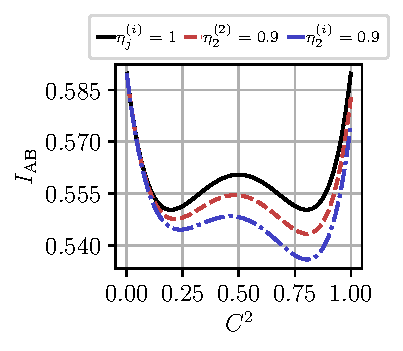
\includegraphics[width=\linewidth, trim={.2cm .3cm .4cm .35cm},clip]{pics/qkd/dhom/IAB.pdf}
\caption[]{$I_{\ind{AB}}$}
        \end{subfigure}
\hfill
        \begin{subfigure}[c]{.3\linewidth}
 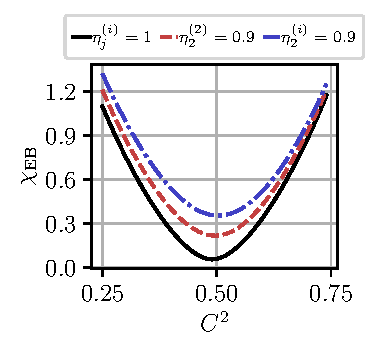
\includegraphics[width=\linewidth, trim={.2cm .3cm .4cm .35cm},clip]{pics/qkd/dhom/chi.pdf}
\caption[]{$\chi_{\ind{EB}}$}
\end{subfigure}
\hfill
    \begin{subfigure}[c]{.3\linewidth}
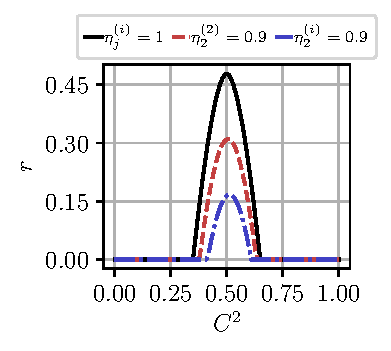
\includegraphics[width=\linewidth, trim={.2cm .3cm .4cm .35cm},clip]{pics/qkd/dhom/r.pdf}
\caption[]{$R$}
        \end{subfigure}
        \caption{(a) Mutual information, (b) Holevo information, and (c) asymptotic secret fraction using double homodyne detection as functions of the signal beam splitter transmission. All other beam splitters are assumed to be balanced. Results are shown for various detector efficiencies; efficiencies not specified in the legend are taken to be unity. Parameters: $V_{\ind{mod}}=1, T=0.95, \xi=10^{-3}, \beta=0.95$.
}
\label{fig:double-homodyne-all}
\end{figure*}
\begin{figure*}
    \centering
    \begin{subfigure}[]{.45\textwidth}
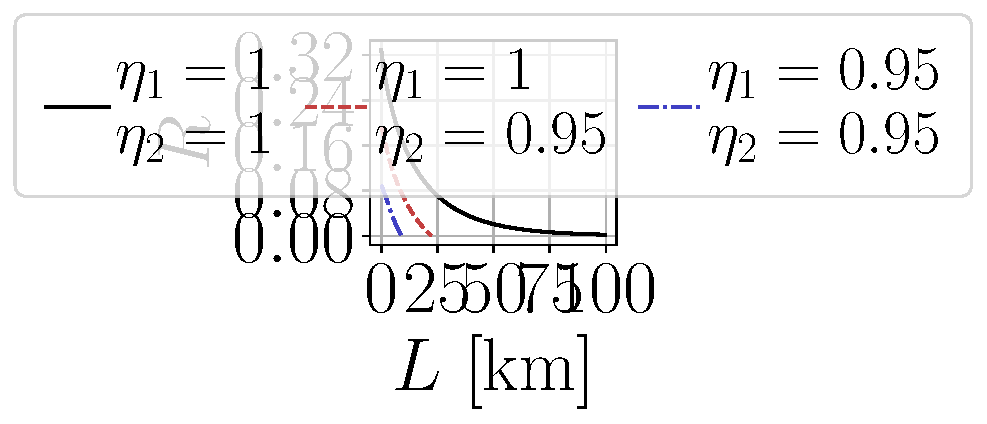
\includegraphics[width=\linewidth]{pics/qkd/hom/r(l).pdf}
\caption[]{Homodyne detection}
\label{fig:hom-r}
        \end{subfigure}
        \begin{subfigure}[]{.45\textwidth}
 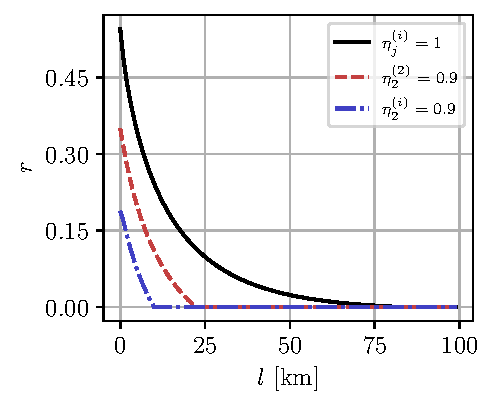
\includegraphics[width=\linewidth]{pics/qkd/dhom/r(l).pdf}
\caption[]{Double homodyne detection}
\label{fig:dhom-r}
\end{subfigure}
\caption{Asymptotic secret fraction as a function of channel length computed for (a) homodyne detection and (b) double homodyne detection, shown for various detector efficiencies. Parameters are $V_{\ind{mod}}=1,T=0.95,\xi=10^{-3}, \beta=0.95$. The losses are assumed to be 20 dB per 100 km.
}
\label{fig:r-of-l-all}
\end{figure*}
%%%%%%%%%%%%%%%%%%%%%%%%%%%%%
\section{Conclusion and discussion}
\label{sec:conclusion}
%%%%%%%%%%%%%%%%%%%%%%%%%%%%

In this paper,
we have studied the effects of asymmetry
introduced by unbalanced beam splitters and different efficiencies of the photodetectors
in photocount statistics of homodyne and double homodyne detection.
We have performed numerical analysis to explore the applicability range for
the Gaussian approximation derived by approximating
the Poisson distributions using the probability density functions of
normally distrbuted random variables.

By using the Gaussian approximation,
we have developed
the method for constructing POVMs of homodyne-based
schematics.
This method is applied to deduce
the expression for the POVM
that generalizes the well-known results to the case of the asymmetric homodyne detection.
This POVM is found to be well defined across all  parameter settings of the scheme
with the excess noise variance modified by the asymmetry 
and incorporates the effect of asymmetry-induced shift of the mean value
(these effects are illustrated in Fig.~\ref{fig:dist-hom}).


We have used the total variational distance~\eqref{eq:stat-dist}, $D_P$,
to quantify the statistical distance between the Skellam and Gaussian distributions
and evaluate the accuracy of the Gaussian approximation across various asymmetry parameters.
It is found that, for the signal mode prepared in the coherent state $\ket{\alpha}$,
the distance increases with $|\alpha|$ (see Fig.~\ref{fig:amp_05}) and,
in the small-amplitude region with $|\alpha|\le 0.1$,
the maximum value of the distance can be estimated at about $0.13$
reached when the local oscillator amplitude $|\alpha_L|$ is in
the vicinity of unity. At $|\alpha_L|>1$, the distance rapidly drops with
the LO amplitude. For example, at $|\alpha|=0.5$,
the distance falls below $0.05$ when the ratio $|\alpha_L|/|\alpha|$ exceeds five
(see Fig.~\ref{fig:amp_01}).

We have found that
(see Figs.~\ref{fig:delta-eta} and~\ref{fig:delta-theta})
dependence of the distance on
the photodetector efficiencies
(the disbalance angle of the beam splitter)
is sensitive to the disbalance of the beam splitter
(photodetector efficiencies).
Thus,
by varying parameters of BS we may achieve the best approximation for given
quantum efficiencies and vice versa.
In general,
our findings indicate that the quality of the agreement between
the exact and approximate photocount distributions varies with
the degree of asymmetry.


Our formalism allows us to easily analyze various homodyne-based schematics. It can be
extended to describe more complex measurement systems.
We have demonstrated this by performing an analysis for
the eight-port asymmetric  double homodyne scheme.
For this scheme,
we have deduced the Gaussian approximation
(see Eqs.~\eqref{eq:Gaussian-8p}--~\eqref{eq:mu_G-i})
and the corresponding POVM expressed in terms of the
projectors onto coherent states (see Eq.~\eqref{eq:povm-hetero}).
As is shown in Fig.~\ref{fig:dh-statistics},
the asymmetry induces effects such as shifts and
anisotropy of the distributions in the photocount difference plane. 

%In contrast to the case of homodyne detection,
%the applicability of
%double homodyne POVM~\eqref{eq:povm-hetero}
%may be broken provided that the beam splitter for the signal mode
%is unbalanced.
%This leads to the effects that deserve a separate publication,
%where we will discuss how to extend our approach to
%this case and related issues.

\textcolor{red}{As shown in the main text, the applicability of double homodyne POVM in the form ~\eqref{eq:povm-hetero} may be broken provided that the beam splitter for the signal mode is unbalanced. To resolve this, an extension to the set of squeezed coherent states is needed (see Eq.~\eqref{eq:Pi_G-gen-x1x2}), leading to explicit dependency of POVM on the squeezing parameter, which is not defined unambiguously. This implies that there are, generally, infinitely many POVMs representing one set of the parameters of double homodyne scheme, and so the squeezing parameter needs additional rule to make the POVM well-defined. Practically, however, ambiguousness of POVM does not matter, as  all of their averages represent the same photon counting difference statistical distribution~\eqref{eq:Gaussian-8p} or, equivalently, quadrature distribution~\eqref{eq:P_G-x1x2}.} \textcolor{blue}{And so, applying our results to CV-QKD (for a comprehensive review see, e.g., Ref.~\cite{laudenbach2018continuous}), choosing any POVM in the form~\eqref{eq:Pi_G-gen-x1x2} would yield the same result for secret fraction, as it is dependent only on variances of quadrature distribution~\eqref{eq:P_G-x1x2}.}

\textcolor{red}{Generalization to complex transmission and reflection
  coefficients for both homodyne and double homodyne is trivial. For
  homodyne, this would entail changing the definition of $\phi$ in
  Eq.{~\eqref{eq:avr-x-phi}} to $\phi'\equiv\phi+\phi_t-\phi_r$, where
  $\phi_t$ and $\phi_r$ are phases of complex transmission and
  reflection coefficients, respectively, and the definition of
  quadrature variable {\eqref{eq:x-def}} would remain unchanged. For
  double homodyne, introducing phases as $\phi_{r,t}^{(j)},
  i\in\{1,2,S,L\}$, a change of $\Re\alpha
  e^{-i\phi}\mapsto\Re\alpha
  e^{-i(\phi-\phi_t^{(L)}-\phi_t^{(S)})}$ and $\Im\alpha
  e^{-i\phi}\mapsto\Im\alpha
  e^{-i(\phi-\phi_r^{(L)}-\phi_r^{(S)})}$ is needed in
  Eq.{~\eqref{eq:P_G-x1x2}}, leaving quadrature variables
  {\eqref{eq:x-1}}, {\eqref{eq:x-2}} unchanged if
  $\phi_r^{(1)}+\phi_t^{(1)}=\phi_r^{(2)}+\phi_t^{(2)}=0$.} 

Note that, according to Appendix~\ref{sec:appendix},
an alternative method based on the Gaussian approximation
for the Bessel function that enters the Skellam distribution
generally leads to  results that are not suitable for dealing with
asymmetry-induced effects in homodyne detection.

\textcolor{red}{Our concluding remark is to put our results in the context of CV-QKD~\cite{zhang2024continuous}. 
The asymmetry effects described in the paper, such as deviations from the ideal 50:50 beam splitter ratio and mismatched detector efficiencies, introduce vulnerabilities into CV-QKD systems. %These flaws not only allow quantum hackers to compromise security but also degrade the system’s performance~\cite{ruiz2023effects}. 
These vulnerabilities can be exploited by adversaries through attack strategies such as the wavelength attack \cite{huang2012wavelength, huang2014quantum} and the homodyne detector blinding \cite{qin2018homodyne} and saturation~\cite{qin2016quantum}. The wavelength attack leverages the wavelength-dependent coupling ratio of fiber beam splitters and can be countered by using proper spectral filtering. Blinding and saturation attacks exploit the saturation behavior of homodyne detectors, and their effectiveness is amplified by receiver imbalance. If the splitting ratio deviates from ideal one, an injected bright pulse more easily displaces the detector output, facilitating saturation and biasing excess noise estimation.} 

\textcolor{blue}{In the main text, we analyzed how measurement asymmetry impacts the performance of CV-QKD system in the untrusted noise scenario, where asymmetry noise is accessible to Eve. In this case, even relatively small asymmetry significantly reduces maximum channel length (see Fig.~\ref{fig:r-of-l-all}).} \textcolor{red}{In trusted-noise CV-QKD~\cite{usenko2016trusted}, if Alice and Bob are unaware of detector’s arms asymmetry, they may misinterpret the increased variance as channel excess noise rather than trusted detector imperfection. This leads to an overestimation of channel excess noise and an underestimation of trusted detector noise. Similar to blinding attacks, this vulnerability can be mitigated by inserting attenuators to balance the detection scheme.}

\textcolor{red}{Despite the existence of countermeasures for the attacks described, implementing analytical corrections based on the formalism developed in this paper would be preferable for accurate security assessment and performance optimization.}

% This method relies on approximating the exact statistics with the Gaussian approximation. We applied this method to
% write POVM for homodyne and double homodyne schemes. For the double homodyne scheme, we have
% encountered a problem with our approach that needs further investigation. Moreover, we have
% studied the applicability of Gaussian approximation in the case of unequal non-unity quantum efficiency
% of photodetectors and unbalanced beam splitters. We have found that the usual approach of
% approximating the Skellam distribution using the asymptotic expansion of the modified Bessel
% function of the first kind is not applicable in the asymmetrical case.


%DeepSeek on homodyne measurements

% Quantum homodyne measurements are a technique used in quantum optics to measure the quadrature
% components of a quantum electromagnetic field.
% These quadrature components represent the amplitude
% and phase of the field, which are crucial for characterizing quantum states of light, such as
% squeezed states or coherent states. 


% ### Key Concepts:

% 1. **Quadrature Components**:
%    - The electric field of a quantum optical mode can be described in terms of two quadrature
%    components, which are analogous to the position and momentum operators in
%    quantum mechanics. 
%    - These components are defined as:
%      \[
%      X = \frac{1}{2}(a + a^\dagger), \quad P = \frac{1}{2i}(a - a^\dagger)
%      \]
%      where \( a \) and \( a^\dagger \) are the annihilation and creation operators, respectively.

% 2. **Homodyne Detection**:
%    - Homodyne detection involves mixing the quantum field of interest with a strong classical
%    reference field (called the local oscillator) at a beam splitter. 
%    - The local oscillator is typically a coherent state with a well-defined phase, which allows the
%    measurement of a specific quadrature of the input field. 
%    - The output beams from the beam splitter are detected by photodetectors, and the difference in
%    the photocurrents is proportional to the quadrature component of the input field that is in phase
%    with the local oscillator. 

% 3. **Phase Sensitivity**:
%    - By adjusting the phase of the local oscillator, different quadrature components of the input
%    field can be measured. For example, if the local oscillator phase is set to zero, the \( X \)
%    quadrature is measured, while a phase shift of \( \pi/2 \) allows measurement of the \( P \)
%    quadrature. 

% 4. **Applications**:
%    - Quantum homodyne measurements are essential for quantum state tomography, where the complete
%    quantum state of a light field is reconstructed from a set of quadrature measurements. 
%    - They are also used in continuous-variable quantum information processing, such as quantum
%    teleportation and quantum key distribution. 

% ### Mathematical Description:

% The homodyne measurement outcome for a quadrature \( X_\theta \) (where \( \theta \) is the phase of the local oscillator) is given by:
% \[
% X_\theta = X \cos \theta + P \sin \theta
% \]


% The probability distribution of the measurement outcomes provides information about the quantum state of the input field.

% ### Summary:

% Quantum homodyne measurements are a powerful tool in quantum optics for probing the quadrature
% components of a quantum electromagnetic field. By using a local oscillator and balanced detection,
% these measurements allow for the precise characterization of quantum states of light, enabling
% advancements in quantum information science and quantum metrology. 


%%%%%%%%%%%%%%%%%%%%%%%%%%%%%%
\section*{Acknowledgements}
The work was supported by the Russian Science Foundation (project No. 24-11-00398).
%%%%%%%%%%%%%%%%%%%%%%%%%%%%%%%%%

\appendix

% %%%%%%%%%%%%%%%%%%%%%%%%%%%%%%
\section{Gaussian approximation from Skellam distribution}
\label{sec:appendix}

%\section{Bessel approximation}%???????
%\label{app:bessel}


The derivation procedure for the Gaussian approximation
outlined in Sec.~\ref{subsec:gauss-hom}
transforms
the photocount difference probability~\eqref{eq:poisson}
into the form of a convolution of the normal distributions
by approximating the Poisson distributions.
In this Appendix,
we discuss an alternative method
where the starting point is the Skellam distribution~\eqref{eq:accurate}.
For convenience, we shall reproduce the expression for
this distribution here:
\begin{align}
  &
\label{eq:Skellam}   
  P(\mu)=e^{-\eta_1|\alpha_1|^2}e^{-\eta_2|\alpha_2|^2}
  \left(\frac{\eta_1|\alpha_1|^2}{\eta_2|\alpha_2|^2}\right)^{\frac{\mu}{2}}
  \notag
  \\
  &
  \times
I_{\mu}\left(2\sqrt{\eta_1\eta_2|\alpha_1|^2|\alpha_2|^2}\right),
\end{align}
where $I_k(z)$ is the modified Bessel function of the first kind
and the amplitudes $|\alpha_{1,2}|$ are given by Eq.~\eqref{eq:amplitudes}.

The method under consideration
(see, e.g. the textbook~\cite{Vogel:bk:2006})
assumes that,
in the strong LO limit, the argument of the modified Bessel function is large
and $I_\mu(z)$ can be
approximated using its asymptotic expansion
taken in the Gaussian form:
\begin{align}
  \label{eq:asymp-A}
  I_\mu(z)\approx\frac{1}{\sqrt{2\pi z}}\exp\left[z-\frac{\mu^2}{2 z}\right].
\end{align}
This formula can be deduced by
performing a saddle-point analysis
for the integral representation of
the Bessel functions~\cite{freyberger1993photon}.

Heuristically, it can also be obtained from
from the lowest order asymptotic expansion for
the Bessel function~\cite{NIST:hndbk:2010}:
$I_{\mu}(z)\approx e^z (1-(4\mu^2-1)/(8z))/\sqrt{2\pi z}$
assuming that, for small values of $x$,
$1-x$ can be replaced with $e^{-x}$
(the factors independent of $\mu$ are not essential because they can be incorporated
into the normalization factor of the Gaussian approximation).


\begin{figure}[ht!]
    \centering
    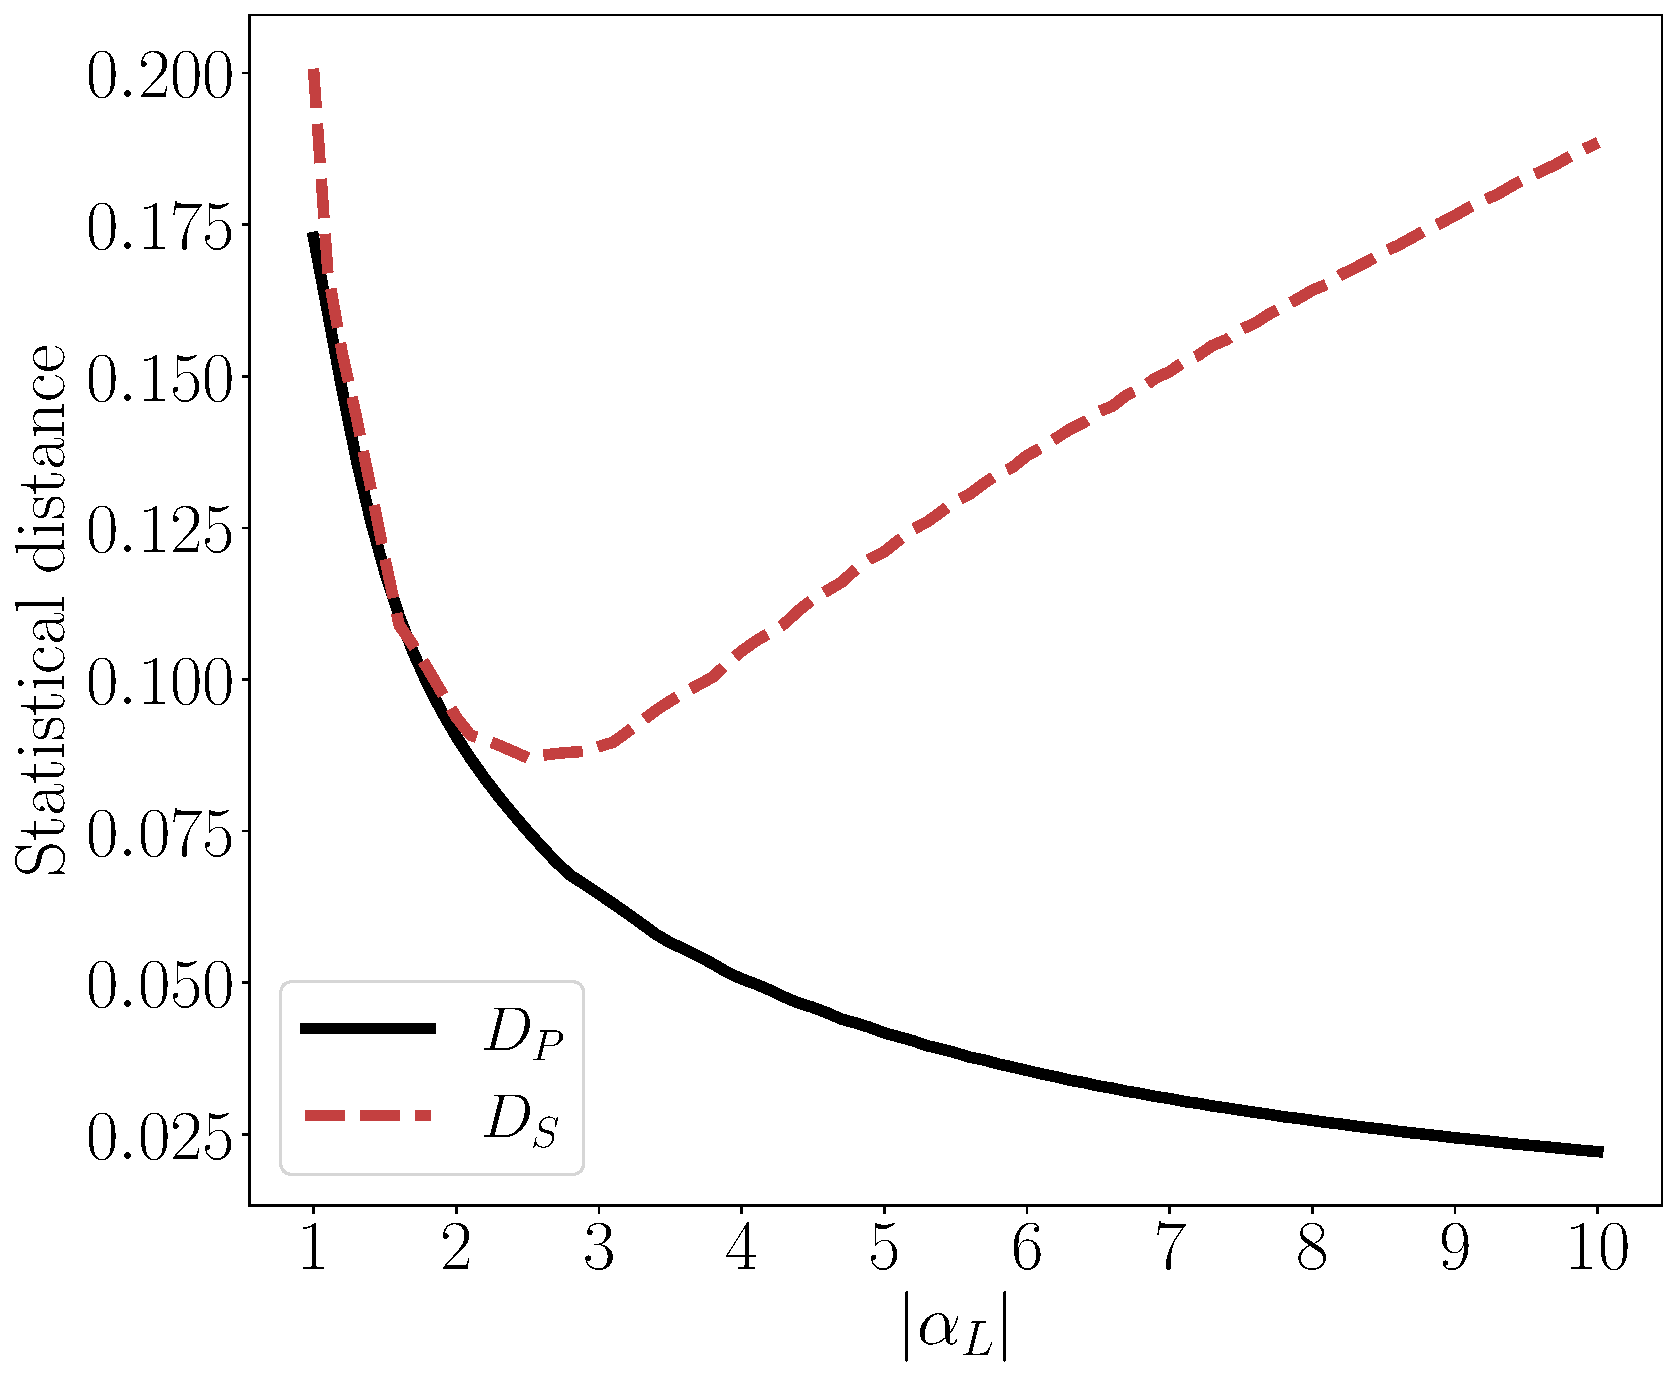
\includegraphics[width=.95\linewidth]{pics/appendix/app_1.pdf}
    \caption{Distances, $D_P=D(\prob,\prob_G)$ and $D_S=D(P,{\prob}_G^{(s)})$, 
      between the Skellam distribution, $P$, and
      two Gaussian approximations, $\prob_G$ (see Eq.~\eqref{eq:Gaussian})
      and  ${\prob}_G^{(s)}$ (see Eq.~\eqref{eq:tPG-mu}), as a function of $|\alpha_L|$
      the beam splitter disbalance angle  at $\delta\theta=15^{\circ}$
$\alpha=1$, and $\eta_1=\eta_2=1$.
      % Note the significant difference (in first decimal places) between the curves, which means that $P_B$
      % becomes incorrect for higher asymmetry
    }
    \label{fig:PGPGs-aL}
\end{figure}


Assuming that $CS\ne 0$ and $|\alpha_L|$ is sufficiently large,
we can use the approximate relations
\begin{align}
  &
    \label{eq:z1-A}
    z=2\sqrt{\eta_1\eta_2}|\alpha_1||\alpha_2|
    \approx
    2CS\sqrt{\eta_1\eta_2}|\alpha_L|^2,
  \\
  &
    \label{eq:z2-A}
    \ln \left(\frac{{\eta_1}|\alpha_1|^2}{{\eta_2}|\alpha_2|^2}\right)^{\frac{\mu}{2}}\approx
    \frac{\mu}{2}\left(
    \ln\frac{\eta_1S^2}{\eta_2C^2}+\frac{\langle\hat{x}_\phi\rangle}{CS|\alpha_L|}\right)
    \end{align}
    to obtain the Gaussian approximation for the Skellam distribution~\eqref{eq:Skellam}
    given by
\begin{align}
  &
  \label{eq:tPG-mu}
        {\prob}_G^{(s)}(\mu)=G(\mu-\tilde{\mu}_G;\tilde{\sigma}_G),
  \\
  &
  \label{eq:tmu_G}
  \tilde{\mu}_G=\sqrt{\eta_1\eta_2}\Bigl[
  CS |\alpha_L|^2\ln\frac{\eta_1S^2}{\eta_2C^2}+
  |\alpha_L|\avr{\hat{x}_{\phi}}
  \Bigr],
  \\
  &
      \label{eq:tsgm_G}
    \tilde{\sigma}_G=
    2CS\sqrt{\eta_1\eta_2}|\alpha_L|^2.
\end{align}



Similar to Eq.~\eqref{eq:Pgood-w-def},
we cast the probabilty~\eqref{eq:tPG-mu}
into the following quadrature form: 
\begin{align}
  &
    \label{eq:tPG-tx}
{\prob}_G^{(s)}(\tilde{x})=\frac{1}{\sqrt{2\pi\tilde{\sigma}_G}}
    \exp \biggl\{-\frac{(\tilde{x}-\avr{\hat{x}_\phi})^2}{2\tilde{\sigma}_x}\biggr\},
  \\
  &
    \label{eq:tld-x}
    \tilde{x}=\frac{\mu}{{\sqrt{\eta_1\eta_2}|\alpha_L|}}-
    CS|\alpha_L|\ln\frac{\eta_1S^2}{\eta_2C^2},
    \\
  &
    \label{eq:tsgm_x}
    \tilde{\sigma}_x=\frac{2CS}{\sqrt{\eta_1\eta_2}},
\end{align}
so that we may follow the line of reasoning
presented in Sec.~\ref{subsec:gauss-hom}
to deduce the POVM
\begin{align}
  &
\label{eq:tpovm}    
    \hat{\Pi}_G^{(s)}=\frac{1}{\sqrt{\eta_1\eta_2}|\alpha_L|}
    \notag
  \\
  &
    \times
    \int \dd x' G(x-x'; \tilde{\sigma}_N)|x',\phi\rangle\langle x',\phi|
\end{align}
with the noise variance
\begin{equation}
  \label{eq:tsigm-N}
  \tilde{\sigma}_N=\tilde{\sigma}_x-1,
  \quad
  0 \le \tilde{\sigma}_x\le \tilde{\sigma}_x^{(\max)}=1/\sqrt{\eta_1\eta_2}.
\end{equation}


\begin{figure}[ht!]
    \centering
    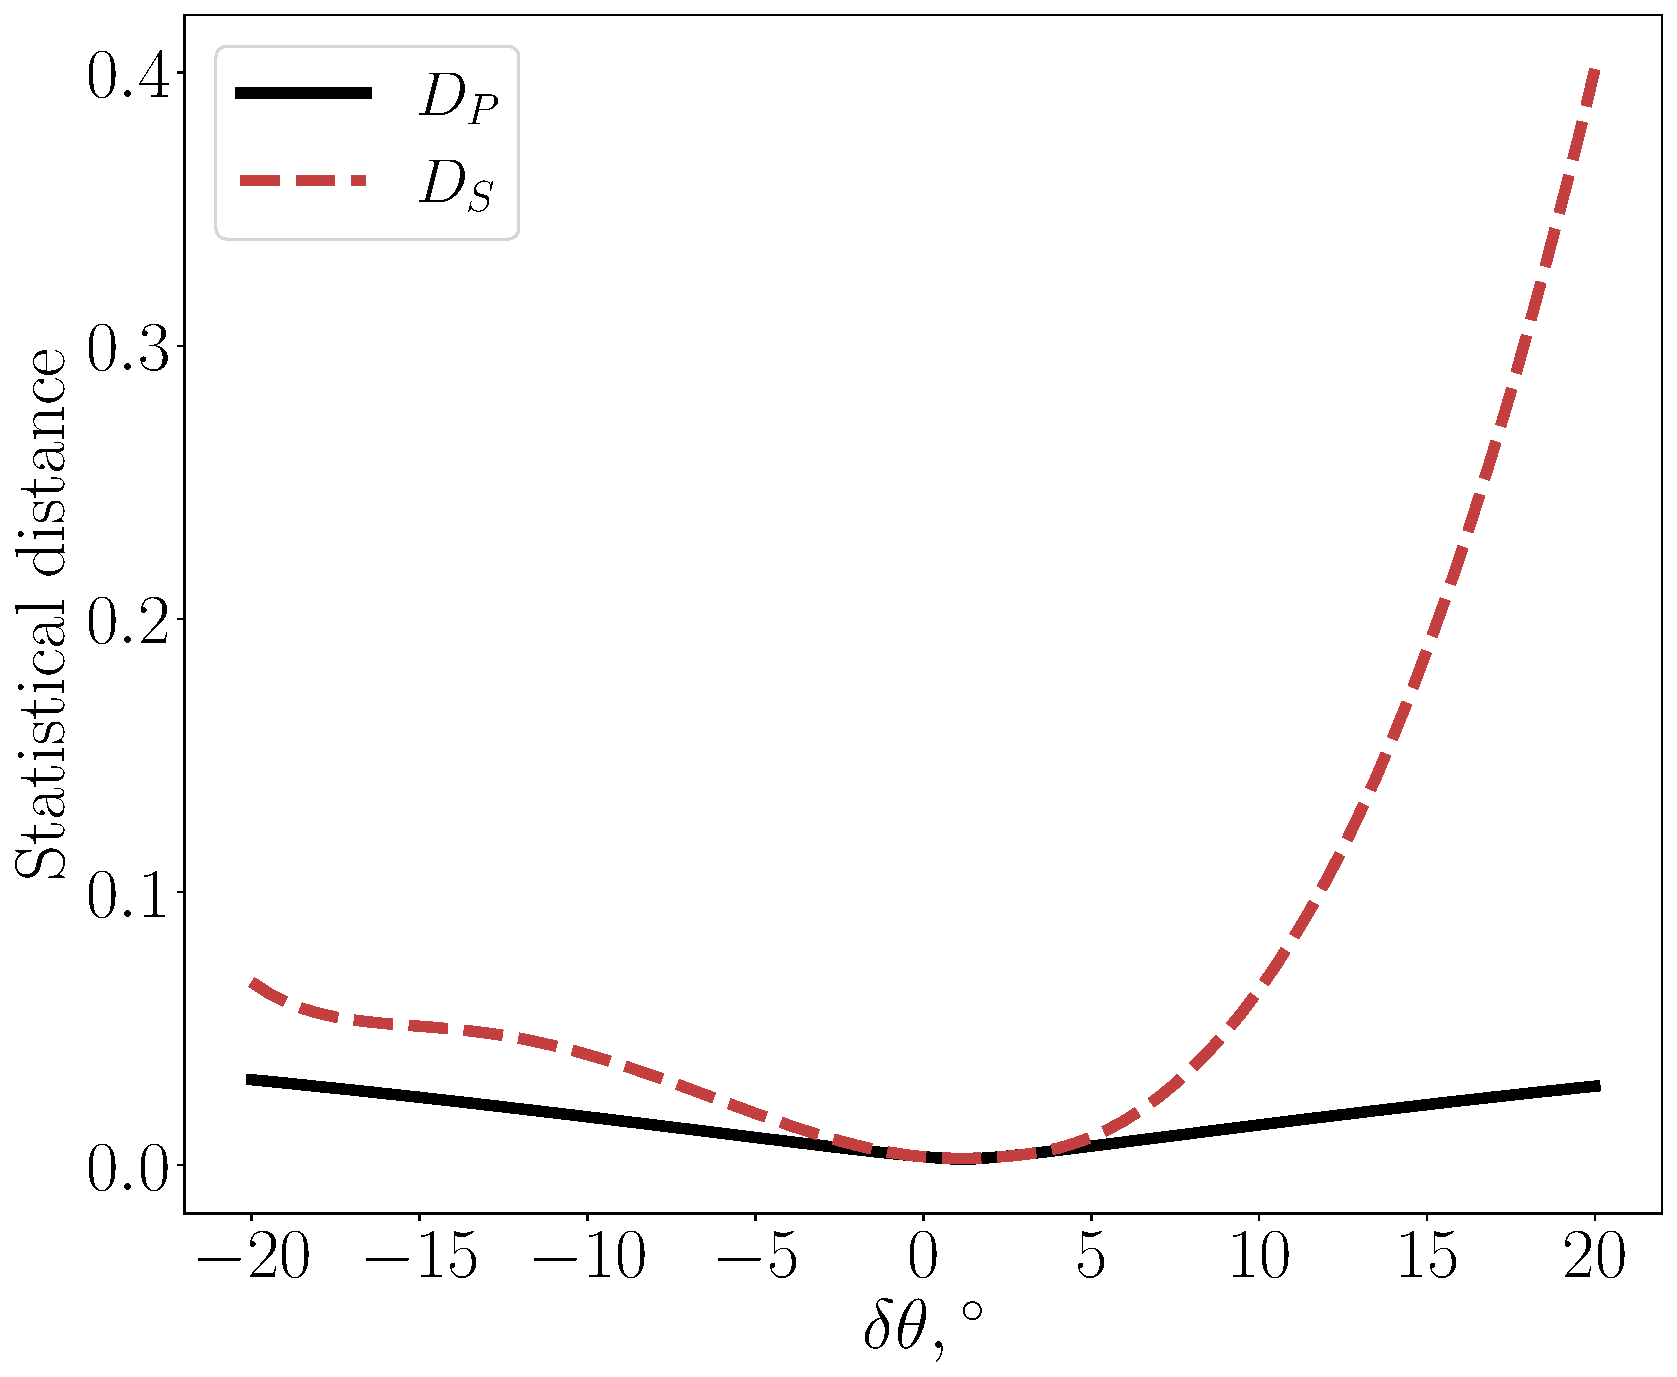
\includegraphics[width=.95\linewidth]{pics/appendix/app_2.pdf}
    \caption{Distances, $D_P=D(\prob,\prob_G)$ and $D_S=D(\prob,\prob_G^{(s)})$, 
      between the Skellam distribution, $P$, and
      two Gaussian approximations, $\prob_G$ (see Eq.~\eqref{eq:Gaussian})
      and  ${\prob}_G^{(s)}$ (see Eq.~\eqref{eq:tPG-mu}), as a function of
      the beam splitter disbalance angle $\delta\theta$ at
$\alpha=1$, $\alpha_L=10$ and
      $\eta_1=\eta_2=1$.
      % Note the significant difference (in first decimal places) between the curves, which means that $P_B$
      % becomes incorrect for higher asymmetry
    }
    \label{fig:PGPGs-dth}
\end{figure}


Note that,
in the symmetric
case with $C=S$ and $\eta_1=\eta_2$,
the Gaussian distributions given by
Eqs.~\eqref{eq:Gaussian} and~\eqref{eq:tPG-mu} are equivalent.
This is no longer the case in the presence of asymmetry effects.

Figure~\ref{fig:PGPGs-aL} demonstrates
that, at $\delta\theta\ne 0$,
by contrast to the distance between $P$ and $\prob_G$,
$D_P=\mathtt{D}(\prob,\prob_G)$ which is a monotonically decreasing function of
$|\alpha_L|$,
the distance
between the Skellam distribution and
the approximate distribution~\eqref{eq:tPG-mu},
$D_S=\mathtt{D}(\prob,\prob_G^{(s)})$,
reveals non-monotonic behaviour and
increases with $|\alpha_L|$ at sufficiently large LO amplitudes.
Referring to Fig.~\ref{fig:PGPGs-dth},
disbalance of the beam splitter
has strong detrimental effect on
the accuracy of the approximation~\eqref{eq:tPG-mu}.

What is more important is
that, by contrast the noise excess variance~\eqref{eq:sgm_N}
which is always positive,
the variance~\eqref{eq:tsigm-N} becomes negative
when $2CS\le \sqrt{\eta_1\eta_2}$.
The latter breaks applicability of Eq.~\eqref{eq:tpovm}
giving an ill-posed POVM.




% This implies that $\sigma$ can be negative for certain combinations of $\eta_{1,2}$ and $\theta$,
% which contradicts the form given in Eq.~\eqref{eq:theform}. Therefore, Eq.~\eqref{eq:Pbad} does not
% fully describe the asymmetrical case, and this is a direct consequence of
% Eq.~\eqref{eq:hole}. 

% Numerical results shown in Fig.~\ref{fig:PB_PG}
% also indicate that $P_G^{(s)}$ is a significantly less
% accurate approximation as compared to $P_G$.

% We can pinpoint the cause of such inaccuracy to
% the approximate terms given by
% Eq.~\eqref{eq:asymp-A} and Eq.~\eqref{eq:z2-A}.
% To this end, we consider the ratio
% % We draw this conclusion from the difference in
% % shifting of exact and approximate formulae, which are described by these terms. To further prove
% % this, we will calculate the relation:
% \begin{align}
%   &
%   \label{eq:ratio}
%     R=\frac{\sqrt{2\pi z}I_{\mu}(z)
%   }{
%     \exp\left[z-\frac{\mu^2}{2z}\right]
%     }
%     \notag
%   \\
%   &
%     \times
%     \frac{\left(\frac{{\eta_1}|\alpha_1|^2}{{\eta_2}|\alpha_2|^2}\right)^{\frac{\mu}{2}}}{\exp\left[\frac{\mu}{2}\left(
%     \ln\frac{\eta_1S^2}{\eta_2C^2}+\frac{\avr{\hat{x}_{\phi}}}{CS|\alpha_L|}\right)
%     \right]},
% \end{align}
% where $z\equiv2\sqrt{\eta_1\eta_2|\alpha_1|^2|\alpha_2|^2}$,
% and evaluate it as a function of $\mu$ depending on the disbalance angle of the beam splitter.
% The results are presented in Fig.~\ref{fig:ratio}.
% It is seen that, at high asymmetry, these approximations do not hold.

% \begin{figure}
%     \centering
%     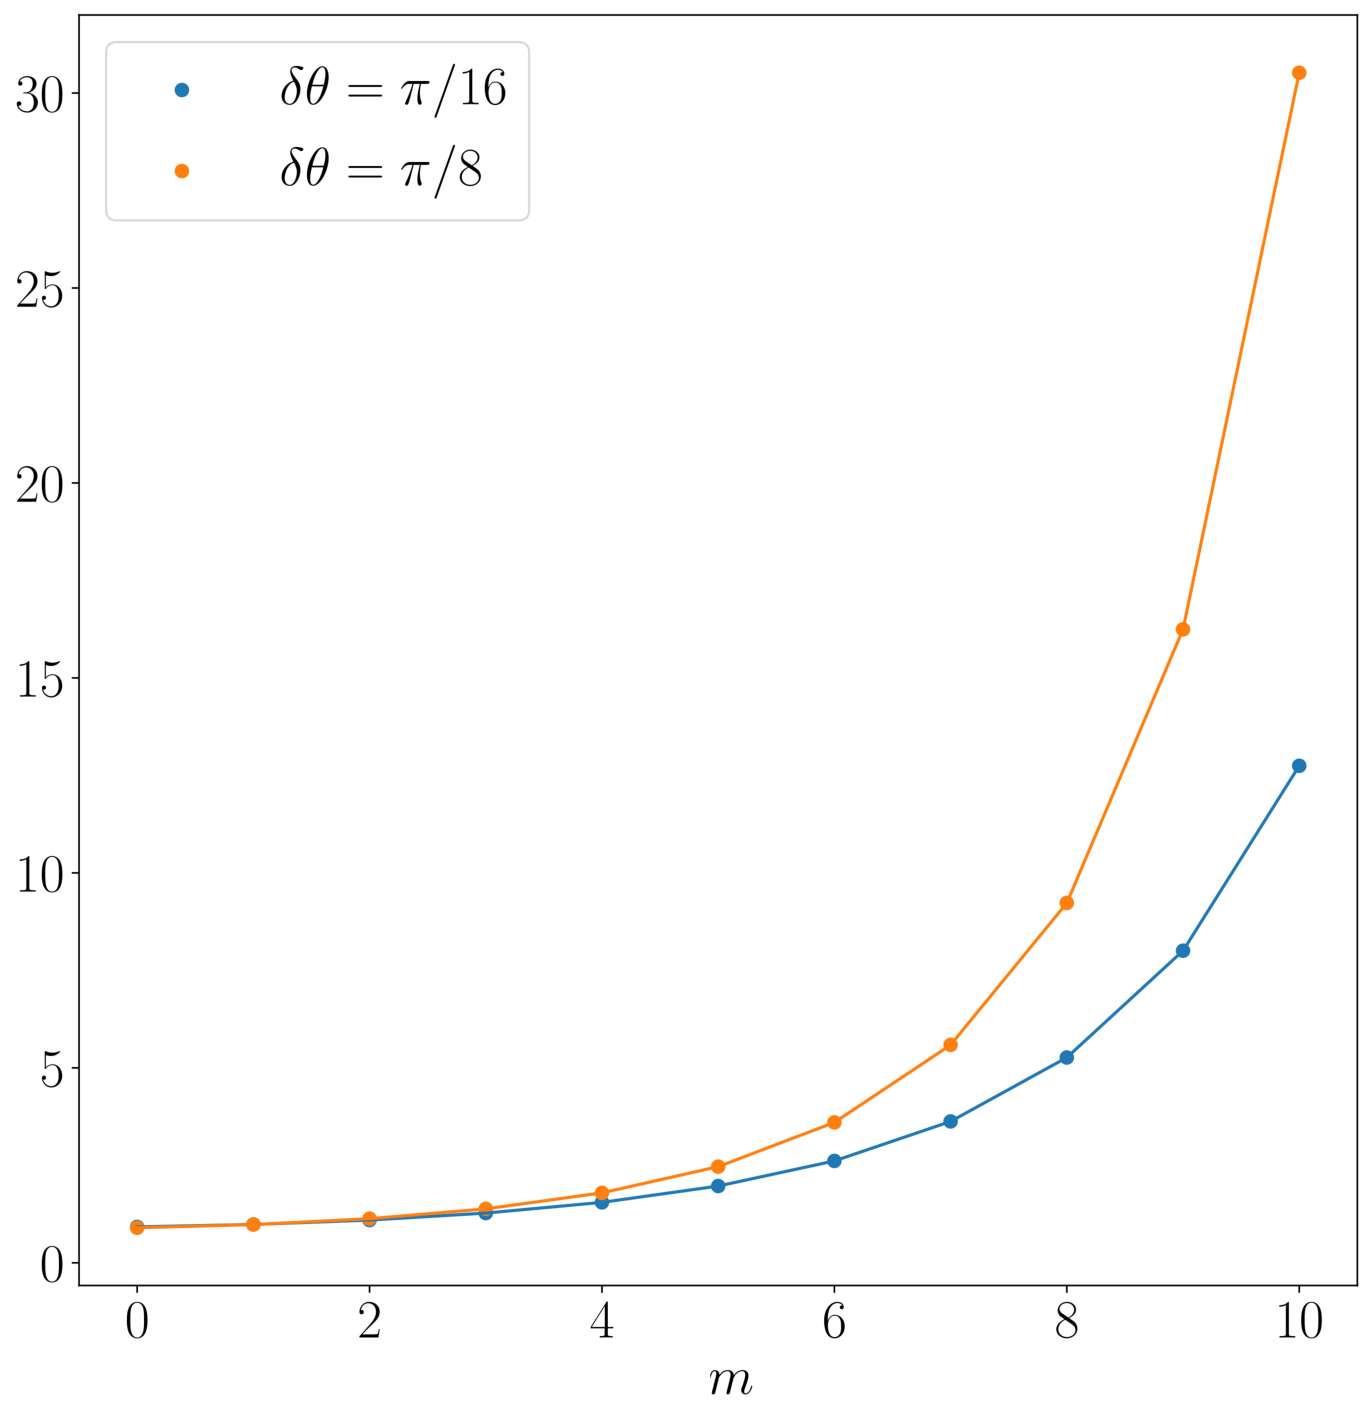
\includegraphics[width=0.75\linewidth]{pics/appendix/relation.pdf}
%     \caption{Ratio given by Eq.~\eqref{eq:ratio} plotted against $\mu$
%       for different values of $\delta\theta$ at $|\alpha_L|=5$,
%       $|\alpha|=0.1$, and $\eta_1=\eta_2=1$.
%       \textbf{Where is the curve with $\delta\theta=0$?}
%       % Significant deviation from unity represents incorrectness of approximations
%       % Eq.~\eqref{eq:hole} and Eq.~\eqref{eq:hole2}.
%     }
%     \label{fig:ratio}
% \end{figure}

% %%%%%%%%%%%%%%%%%%%%%%

%\bibliography{quant,my_papers,refs}
\bibliography{quant,refs,homodyne,math}

\end{document}



%%% Local Variables:
%%% mode: latex
%%% TeX-master: t
%%% End:
